% ============================================================
% 基于大语言模型与可解释机器学习的风电场选址多任务融合框架
% 终稿 — pdfLaTeX编译
% ============================================================
\documentclass[12pt, a4paper]{article}

\usepackage[T1]{fontenc}
\usepackage{newtxtext,newtxmath}
\usepackage{url}
\usepackage{CJKutf8}
\usepackage[top=2.5cm, bottom=2.5cm, left=3cm, right=3cm]{geometry}
\usepackage{setspace}
\onehalfspacing
\usepackage{amsmath, amssymb, bm}
\usepackage{graphicx}
\usepackage{booktabs}
\usepackage{tabularx}
\usepackage{multirow}
\usepackage{array}
\usepackage{float}
\usepackage[labelfont=bf, font=small]{caption}
\usepackage{xcolor}
\usepackage[colorlinks=true, linkcolor=blue!70!black,
            citecolor=blue!70!black, urlcolor=blue!70!black]{hyperref}
\usepackage[numbers, sort&compress]{natbib}
\bibliographystyle{unsrtnat}
\usepackage{enumitem}
\usepackage{indentfirst}
\usepackage{fancyhdr}
\pagestyle{fancy}
\fancyhf{}
\rhead{\small \begin{CJK}{UTF8}{gbsn}风电场选址多任务融合框架\end{CJK}}
\lhead{\small \begin{CJK}{UTF8}{gbsn}中国风电选址\end{CJK}}
\cfoot{\thepage}
\setlength{\parindent}{2em}

\graphicspath{{./}}

% ============================================================
\begin{document}
\begin{CJK}{UTF8}{gbsn}

\title{\textbf{基于大语言模型与可解释机器学习的\\[0.3em]
风电场选址多任务融合框架}\\[0.5em]
{\large ——以中国73--135$^\circ$E、37--50$^\circ$N区域为例}}
\author{（作者）}
\date{}
\maketitle
\thispagestyle{fancy}

% ── 摘要 ─────────────────────────────────────────────────
\begin{abstract}
风电场选址需要在气象资源、工程可行性与政策合规性之间进行协同优化。然而，现有方法通常将政策约束简化为二值掩码，无法刻画监管文本中“鼓励、限制、禁止”等细粒度语义信息，从而限制了政策因素在数据驱动决策中的有效融合。

为解决这一问题，本文提出一种双流跨模态学习框架，在统一可训练架构中联合建模政策语义与地理空间数值特征。其中，政策语义流通过对预训练语言模型进行参数高效微调，从中文监管文本中提取省级密集语义表示；数值特征流则对来自ERA5再分析数据、数字高程模型及OpenStreetMap的气象、地形与基础设施等异质变量进行编码。跨模态注意力机制使数值特征能够主动查询政策语义信息，并通过Sigmoid门控实现自适应融合。同时，采用多任务学习框架联合优化场址适宜性排序、风能潜力评估与工程合规性预测。

在覆盖中国北方13197个ERA5格点的实验中，引入政策语义后模型性能显著提升，在控制省份固定效应后AUC提高0.079（p = 0.002）。进一步地，本文提出省级空间优先级正则化（PSPR）的概念，揭示政策信号并非在格点尺度上直接贡献预测，而是通过重塑行政边界尺度的先验适宜性分布发挥作用。这一发现解释了SHAP分析中局部贡献接近于零的现象，并与中国风电开发的分层治理结构相一致。门控权重的空间异质性分析进一步表明，模型能够执行“数值引导的语义检索”，在重点开发区域表现出更强的政策依赖性。

在独立验证中，该框架取得0.897的AUC，高适宜区域主要分布于新疆、内蒙古、甘肃和吉林，与国家风电发展规划高度一致。研究表明，将政策语义作为可学习表示引入模型，可实现更加符合现实决策逻辑的风电场选址，为监管约束下的数据驱动能源规划提供了一种新的方法范式。
\textbf{数值引导的语义检索}。独立验证AUC=0.8970，高适宜区集中于
新疆、内蒙古、甘肃和吉林，与国家五年规划的风电重点区域高度一致。

\bigskip
\noindent\textbf{关键词：}风电场选址；大语言模型；跨模态注意力；%
多任务学习；SHAP；中国
\end{abstract}

\newpage
\tableofcontents
\newpage

% ============================================================
\section{引言}
% ============================================================

中国风电装机规模持续扩张，选址决策的技术复杂度也随之上升。在
格点尺度同步评估气象资源、工程可及性与政策合规性，是制约风电
高质量开发的核心难题。本文提出一种将政策文本语义与气象数值特征
融合的选址框架，通过多层次评估协议检验其有效性。

截至2024年底，全国风电装机容量达5.21亿千瓦，占全球总装机量的
45.8\%~\cite{ruan2025,he2023}，风光合计装机已超越火电~\cite{ruan2025}。在"双碳"战略目标驱动下，《"十四五"可再生
能源发展规划》~\cite{ndrc2022}和《"十五五"规划纲要》~\cite{ndrc2026}
均明确提出大幅扩张风电装机规模。当前，风电开发的空间扩张正面临多重
约束：气象资源高度集中于西北、华北、东北地区，而电力消费中心位于
东部沿海，跨区输送成本与弃风率居高不下；与此同时，生态红线、永久
基本农田、军事管理区等禁止建设区域的刚性约束日趋收紧，省级和地市级
差异化政策进一步增加了选址的合规难度~\cite{zhong2022}。在此背景下，
选址方法需要能够同步处理数值空间特征与非结构化政策文本，而现有框架
在这一方面存在显著局限。

现有选址方法大致分为三类，各有其适用范围与不足。传统GIS多准则决策
分析方法依赖人工设定的准则权重，权重的主观性导致结果对赋权方案高度
敏感，且无法将政策文件的语义内容直接纳入模型~\cite{xu2020,wu2022}。
纯机器学习框架在判别精度上取得了显著进展：Bilgili等~\cite{bilgili2024}
以XGBoost结合SHAP实现96.07\%准确率，Chen等~\cite{chen2026}在中国区域
尺度上构建了时空概率分布模型；但上述研究均将政策合规性简化为预处理
阶段的二值掩码，丢失了监管文本中鼓励、限制、禁止等不同意图之间的
语义梯度。自然语言处理方法为从非结构化文本中提取约束信息提供了新
路径，Buster等~\cite{buster2024}和Li等~\cite{li2023}分别将BERT应用于
法律文件和能源政策分析，但上述研究均未将编码结果与空间数值特征融合，
也未形成统一的可训练选址框架。

三类方法的局限指向同一个核心缺口：如何在单一可训练架构中，让政策文本
的语义信息真正参与空间决策，而不是停留在预处理阶段的规则过滤。现有工作
尚无将政策语义向量与ERA5数值特征进行跨模态融合的先例，在格点尺度量化
中国风电政策省际异质性的研究也基本空白。在此背景下，本文提出以下贡献：

\begin{enumerate}[leftmargin=2em]
  \item \textbf{跨模态融合框架：}首个将BERT+LoRA政策语义编码与ERA5
        数值特征通过跨注意力机制在统一可训练架构中融合的中国风电
        选址框架，优先适用于三北地区。TabTransformer作为异质数值
        特征的上下文编码机制，跨模态注意力作为政策语义与数值特征
        动态交互的实现机制，共同支撑政策语义的空间映射能力；
  \item \textbf{GradNorm多任务联合优化：}在融合表示之上引入GradNorm
        自适应损失平衡，作为场址排名、风能资源评估与工程及政策合规
        三个目标联合优化的训练机制，避免单目标方法中任务间权衡缺失
        的问题；
  \item \textbf{高分辨率适宜性图：}生成覆盖73--135$^\circ$E、
        37--50$^\circ$N的全国尺度适宜性地图，共13197个格点，
        分辨率0.1$^\circ$，为国家级预筛选提供空间决策支持；
  \item \textbf{SHAP可解释性分析：}通过SHAP量化政策特征贡献的
        省际空间异质性，揭示模型决策逻辑并支撑融合框架设计的
        合理性；
  \item \textbf{严格四实验评估体系：}区分地理泛化能力、政策流
        增量贡献与独立SCADA验证三个维度，为方法可靠性提供
        多层次证据。
\end{enumerate}

% ============================================================
\section{文献综述}
% ============================================================

风电场选址研究沿三条技术路线发展：多准则决策分析侧重政策权重建模，
机器学习侧重数值特征挖掘，自然语言处理侧重监管文本语义提取。三者各有
成熟的应用场景，但在如何将三类信息统一纳入可训练框架这一问题上，
现有工作尚未给出有效答案。

\subsection{多准则决策分析方法}

多准则决策分析方法是风电选址中应用最为广泛的传统框架，主要包括
层次分析法、逼近理想解排序法及其模糊扩展变体~\cite{xu2020,wu2022}。
这类方法将风速、地形坡度、到电网距离、土地利用类型等准则纳入加权
评分体系，通过专家赋权后对候选区域进行综合排序。其优势在于框架
透明、计算简便，易于与GIS空间分析工具集成，因此在省级或区域级
选址规划中得到广泛应用。

该框架存在两个根本性局限。其一是权重主观性问题：不同专家对同一
准则的重要性判断可能存在显著差异，赋权方案的差异对最终适宜性评分
的影响不可忽视，结果的可重复性因此受到限制~\cite{wu2022,xu2020}。
其二是政策信息的语义损失问题：现有研究将政策约束简化为二值掩码
或离散分级标量，完全依赖研究者对政策原文的主观解读，无法捕捉
鼓励、限制、禁止等不同监管意图之间的语义梯度。中国风电政策语言
的情境依赖性极强，同一区域在不同文件中可能同时出现鼓励开发和限制
建设的条款，二值掩码无力表达这种复杂的语义结构。

\subsection{机器学习方法}

机器学习方法在风电选址判别精度上取得了显著进展，逐步突破了多准则
决策分析框架的线性加权局限。近年来，集成学习和梯度提升方法成为主流。
Bilgili等~\cite{bilgili2024}以XGBoost结合SHAP在土耳其风电选址数据集
上实现96.07\%准确率；其后续工作~\cite{bilgili2024xai}进一步引入七种ML算法与
信息增益特征选择，验证了风速、输电线路距离和高程为选址主导因素。
Jurasz等~\cite{jurasz2025}在波兰以MLP对28个时空环境特征建模，测试集
准确率达91\%，表明数据驱动方法在欧洲地区的选址适用性。Chen等~\cite{chen2026}在中国区域尺度上构建了风电与
光伏选址的时空概率分布模型，量化了多尺度时空因素对选址决策的影响。

上述研究存在一个共同的结构性局限：政策合规性均被处理为预处理阶段的
二值掩码，在模型训练前通过空间叠加排除禁建区，而非作为可学习特征
纳入模型。这一处理方式丢失了中国能源政策语言中大量情境性语义信息——
"鼓励在戈壁荒漠建设大型风电基地"与"严格限制在生态敏感区建设风电"
这两类条款对格点选址判断具有截然不同的语义贡献，但在二值掩码框架下
均被简化为允许或禁止的二元判断。现有机器学习研究还普遍缺乏独立的
实测数据验证，多依赖行政边界标签或专家判断作为训练标签，存在一定的
循环性风险。

\subsection{NLP与大语言模型方法}

自然语言处理技术为从非结构化政策文本中提取选址约束信息提供了新路径。
Buster等~\cite{buster2024}以BERT为基础模型，从美国2500余份县级区划
法律文件中自动提取风机退距规定，准确率达85至90\%，显著降低了人工
解读大规模法律文本的成本。Li等~\cite{li2023}将BERT分类器应用于中文
能源政策文本分析，实现了对政策支持强度的自动量化。

这一研究方向存在两个关键局限。其一是空间映射缺失：上述研究均将NLP
编码结果以报告或统计摘要的形式输出，未将编码结果映射至具体的候选
场址格点，无法直接用于空间选址决策；现有研究无法从政策原文中自动
提取鼓励、限制、禁止等监管意图的语义梯度，本研究的BERT+LoRA方案
正是针对这一局限提出的改进。其二是联合训练缺失：政策文本编码与空间
数值特征的融合通过人工后处理完成，而非在统一可训练架构中联合优化，
两类信息之间的交互关系无法被模型自适应学习。GPT-4类方法还面临推理成本高、结果不可重复的问题，无法针对特定
领域数据进行梯度优化；最新研究表明LLM在环境许可审查等监管推理任务
上仍面临显著挑战~\cite{nepa2025}。
相比之下，基于BERT+LoRA的参数高效微调方法在保持预训练语义知识的
同时，能够以极低的计算成本适配特定领域的分类任务~\cite{hu2022}，
更适合构建可重复的统一选址框架。

\subsection{研究空白}

综合上述三类方法的局限，现有风电选址研究在以下六个维度存在系统性
空白（表~\ref{tab:gap}）。多准则决策分析方法在空间分析上成熟，
但政策建模依赖人工标量；机器学习方法在数值特征挖掘上领先，但政策
信息被简化为后处理掩码；自然语言处理方法在语义提取上取得突破，
但缺乏与空间数值特征的融合机制。三类方法的优势互补性正指向本研究
的核心设计动机：需要一个能够同时编码数值特征与政策文本语义、并通过
可学习注意力机制实现两者自适应融合的统一框架。

从评估严谨性看，现有研究普遍缺乏在真实运行场址上的独立外部验证。
SCADA实测数据提供了独立于训练过程的客观验证基准，目前尚未被系统
应用于风电选址框架的评估。

\begin{table}[H]
\centering
\caption{现有方法与本文框架的研究空白对比}
\label{tab:gap}
\small
\begin{tabularx}{\textwidth}{lXX}
\toprule
\textbf{维度} & \textbf{现有研究} & \textbf{本文} \\
\midrule
政策建模 & 定性或二值掩码 &
  BERT+LoRA密集语义向量，省级空间映射 \\
数值特征 & GIS单模态，专家赋权 &
  TabTransformer（16个ERA5+DEM+OSM特征） \\
融合机制 & 无（独立流或规则拼接） & 跨注意力+门控融合 \\
多任务学习 & 单目标优化 & GradNorm三任务头 \\
真实标签来源 & 专家判断或行政边界 &
  OSM风机GPS聚类 + SCADA独立验证 \\
空间范围 & 省级或区域级 &
  全国尺度（13197格点，0.1$^\circ$） \\
\bottomrule
\end{tabularx}
\end{table}

% ============================================================
\section{研究区域与数据}
% ============================================================

本研究的数据体系由气象特征、地形特征、工程特征和政策语料库四部分
构成，覆盖73--135$^\circ$E、37--50$^\circ$N的13197个ERA5陆地格点。
以下依次介绍各类数据的来源、范围与特征统计。

\subsection{研究区域}

研究区域以0.1$^\circ$分辨率共获得13197个ERA5陆地格点，覆盖新疆、
甘肃河西走廊、内蒙古草原、黑龙江、山东半岛等风电重点省份。
图~\ref{fig:study_area}以颜色深浅表示ERA5 100\,m高度年均风速的空间
分布，红色星形标注九个独立验证风电场的推断位置；喀什场址因ERA5相关系数
仅为0.154，坐标推断可靠性不足，已从验证集排除。新疆哈密至吐鲁番走廊和内蒙古高原呈现明显的高风速区域，
是本研究重点关注的风电潜力区。

\begin{figure}[H]
\centering
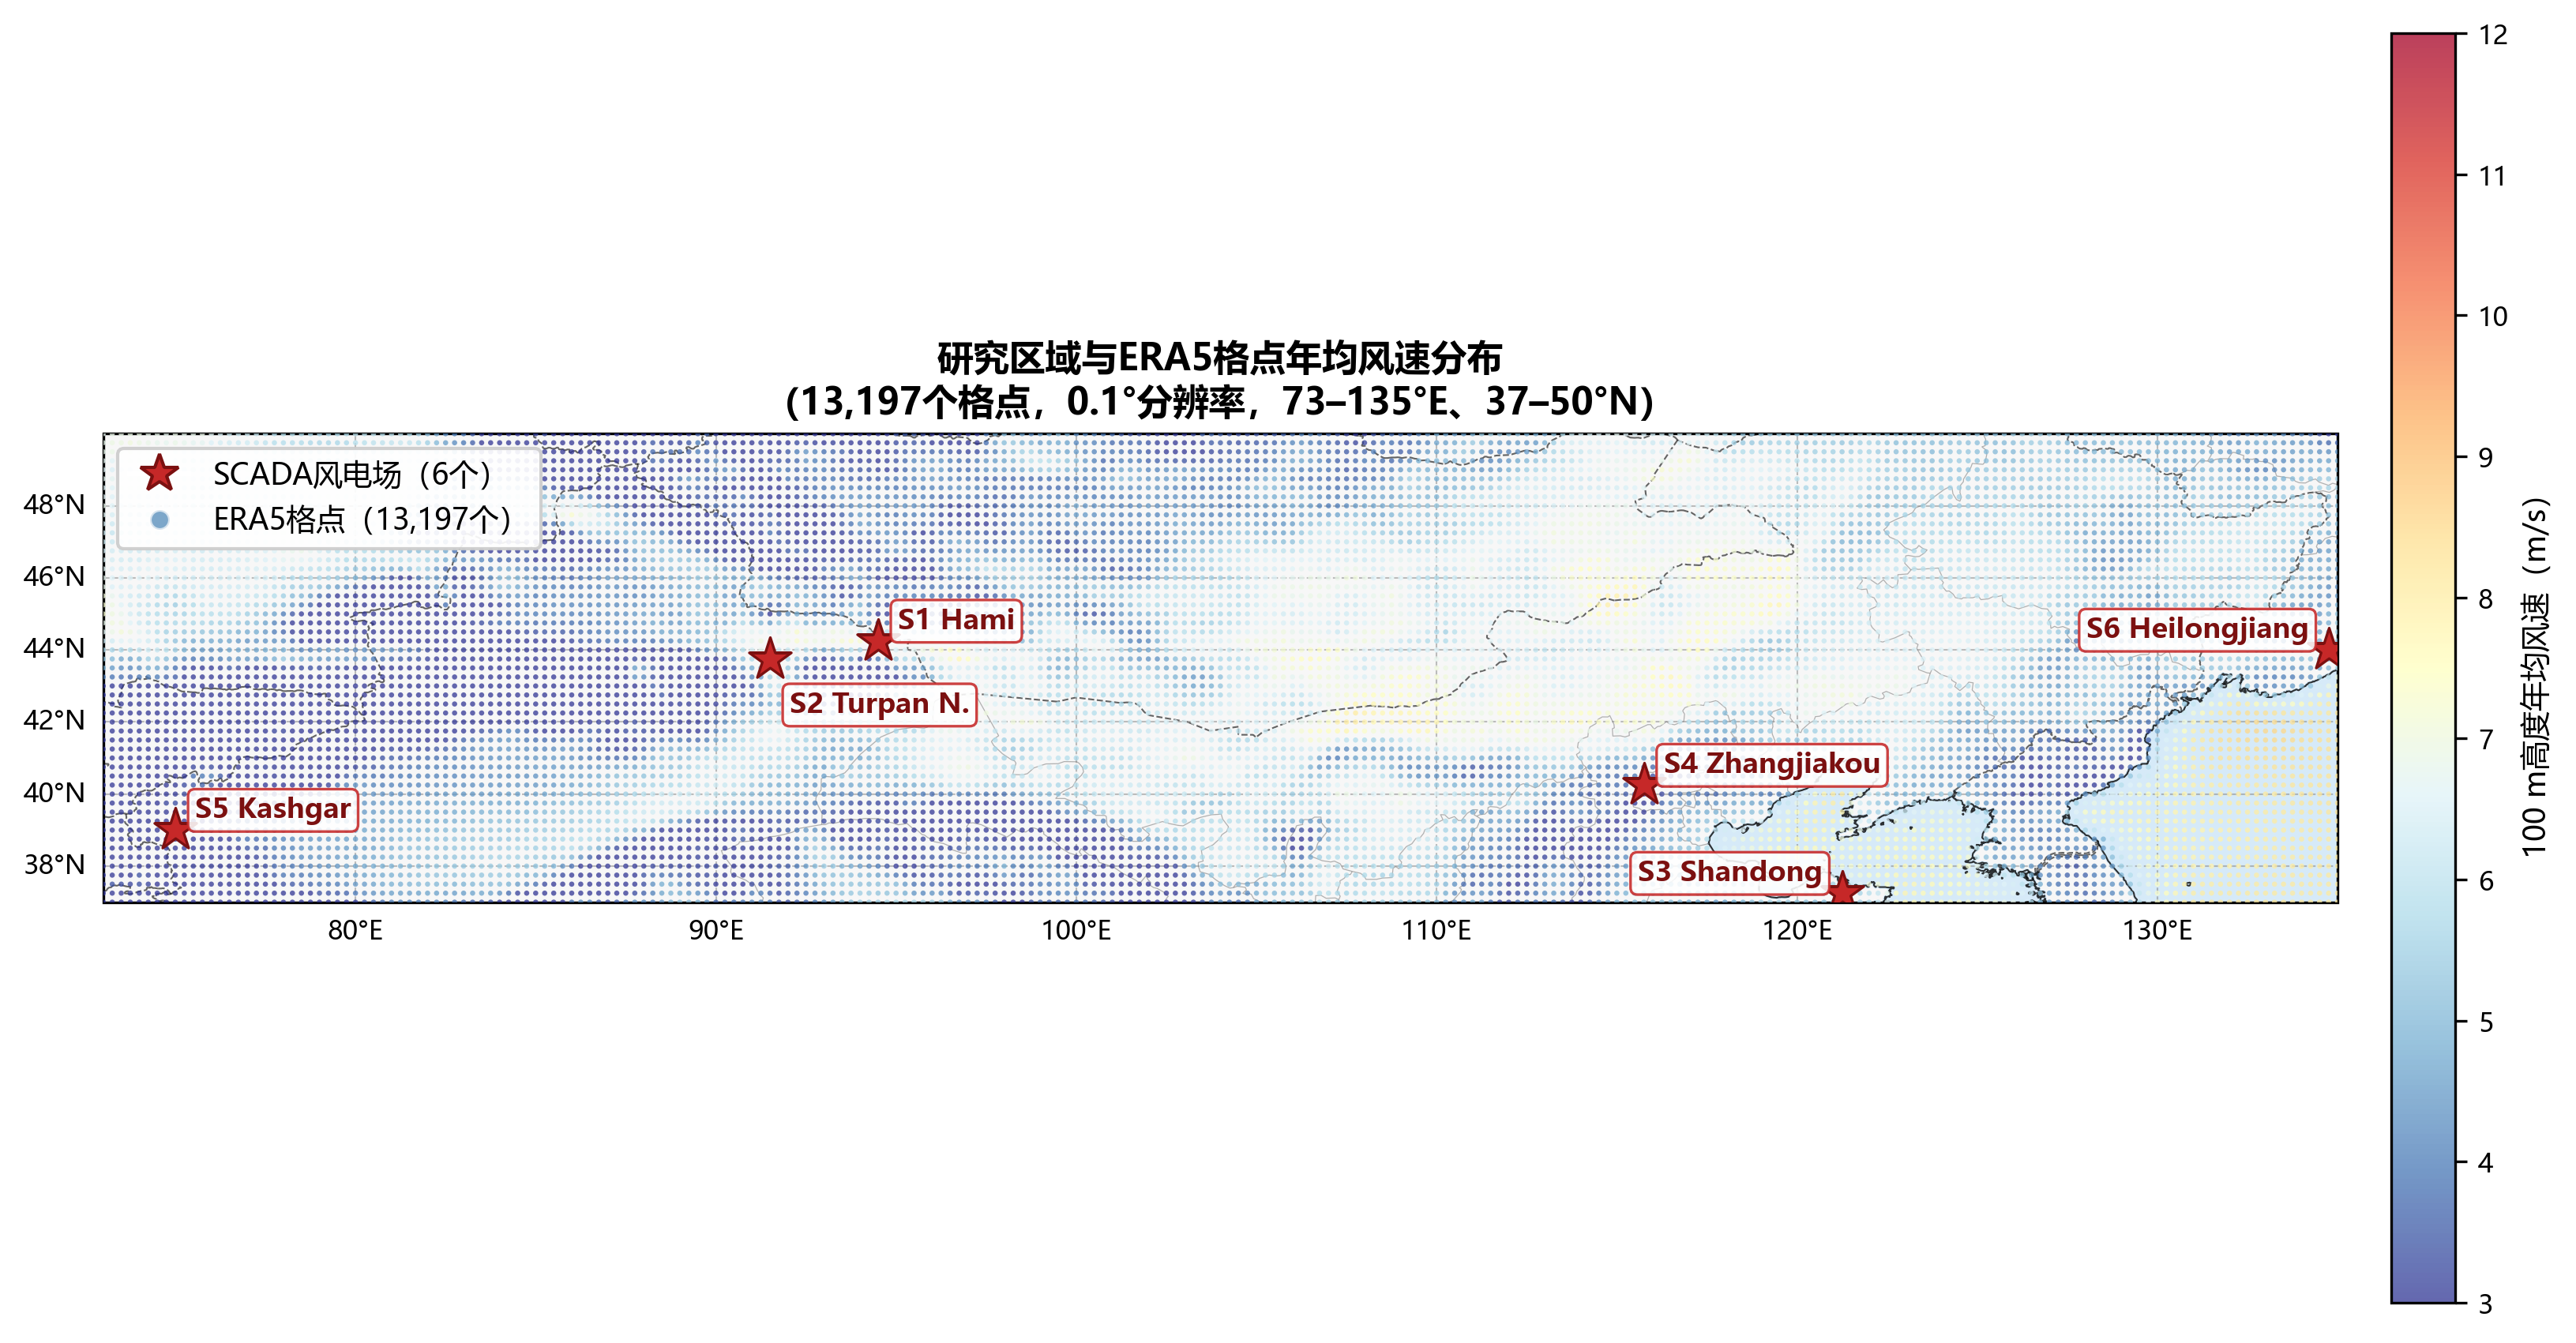
\includegraphics[width=0.95\textwidth]{fig1_1_study_area.jpeg}
\caption{研究区域与ERA5格点年均风速分布}
\label{fig:study_area}
\end{figure}

\subsection{ERA5气象特征}

从2018至2025年100\,m高度的ERA5再分析数据中提取9个风能特征（
ERA5在复杂地形的降尺度不确定性参见Ding等~\cite{superres2025}）：年均
风速、风速标准差、风功率密度、风速第75百分位数、年均有效发电小时数
（风速超过3\,m/s）、年均高效发电小时数（风速超过10\,m/s）、季节
变异系数、威布尔$k$参数和威布尔$c$参数。

\subsection{地形特征}

从0.1$^\circ$分辨率DEM提取4个地形特征，全部13197个格点均无缺失值，
如图~\ref{fig:terrain}所示。高程均值为1154\,m，最高达5327\,m；
坡度经弧度至度转换后均值为0.86$^\circ$，最大值20.8$^\circ$，
坡度超过5$^\circ$的格点占比1.4\%；地形位置指数范围为$-2{,}057$至
$+1{,}955$\,m；粗糙度均值419\,m，最大6026\,m。

\begin{figure}[H]
\centering
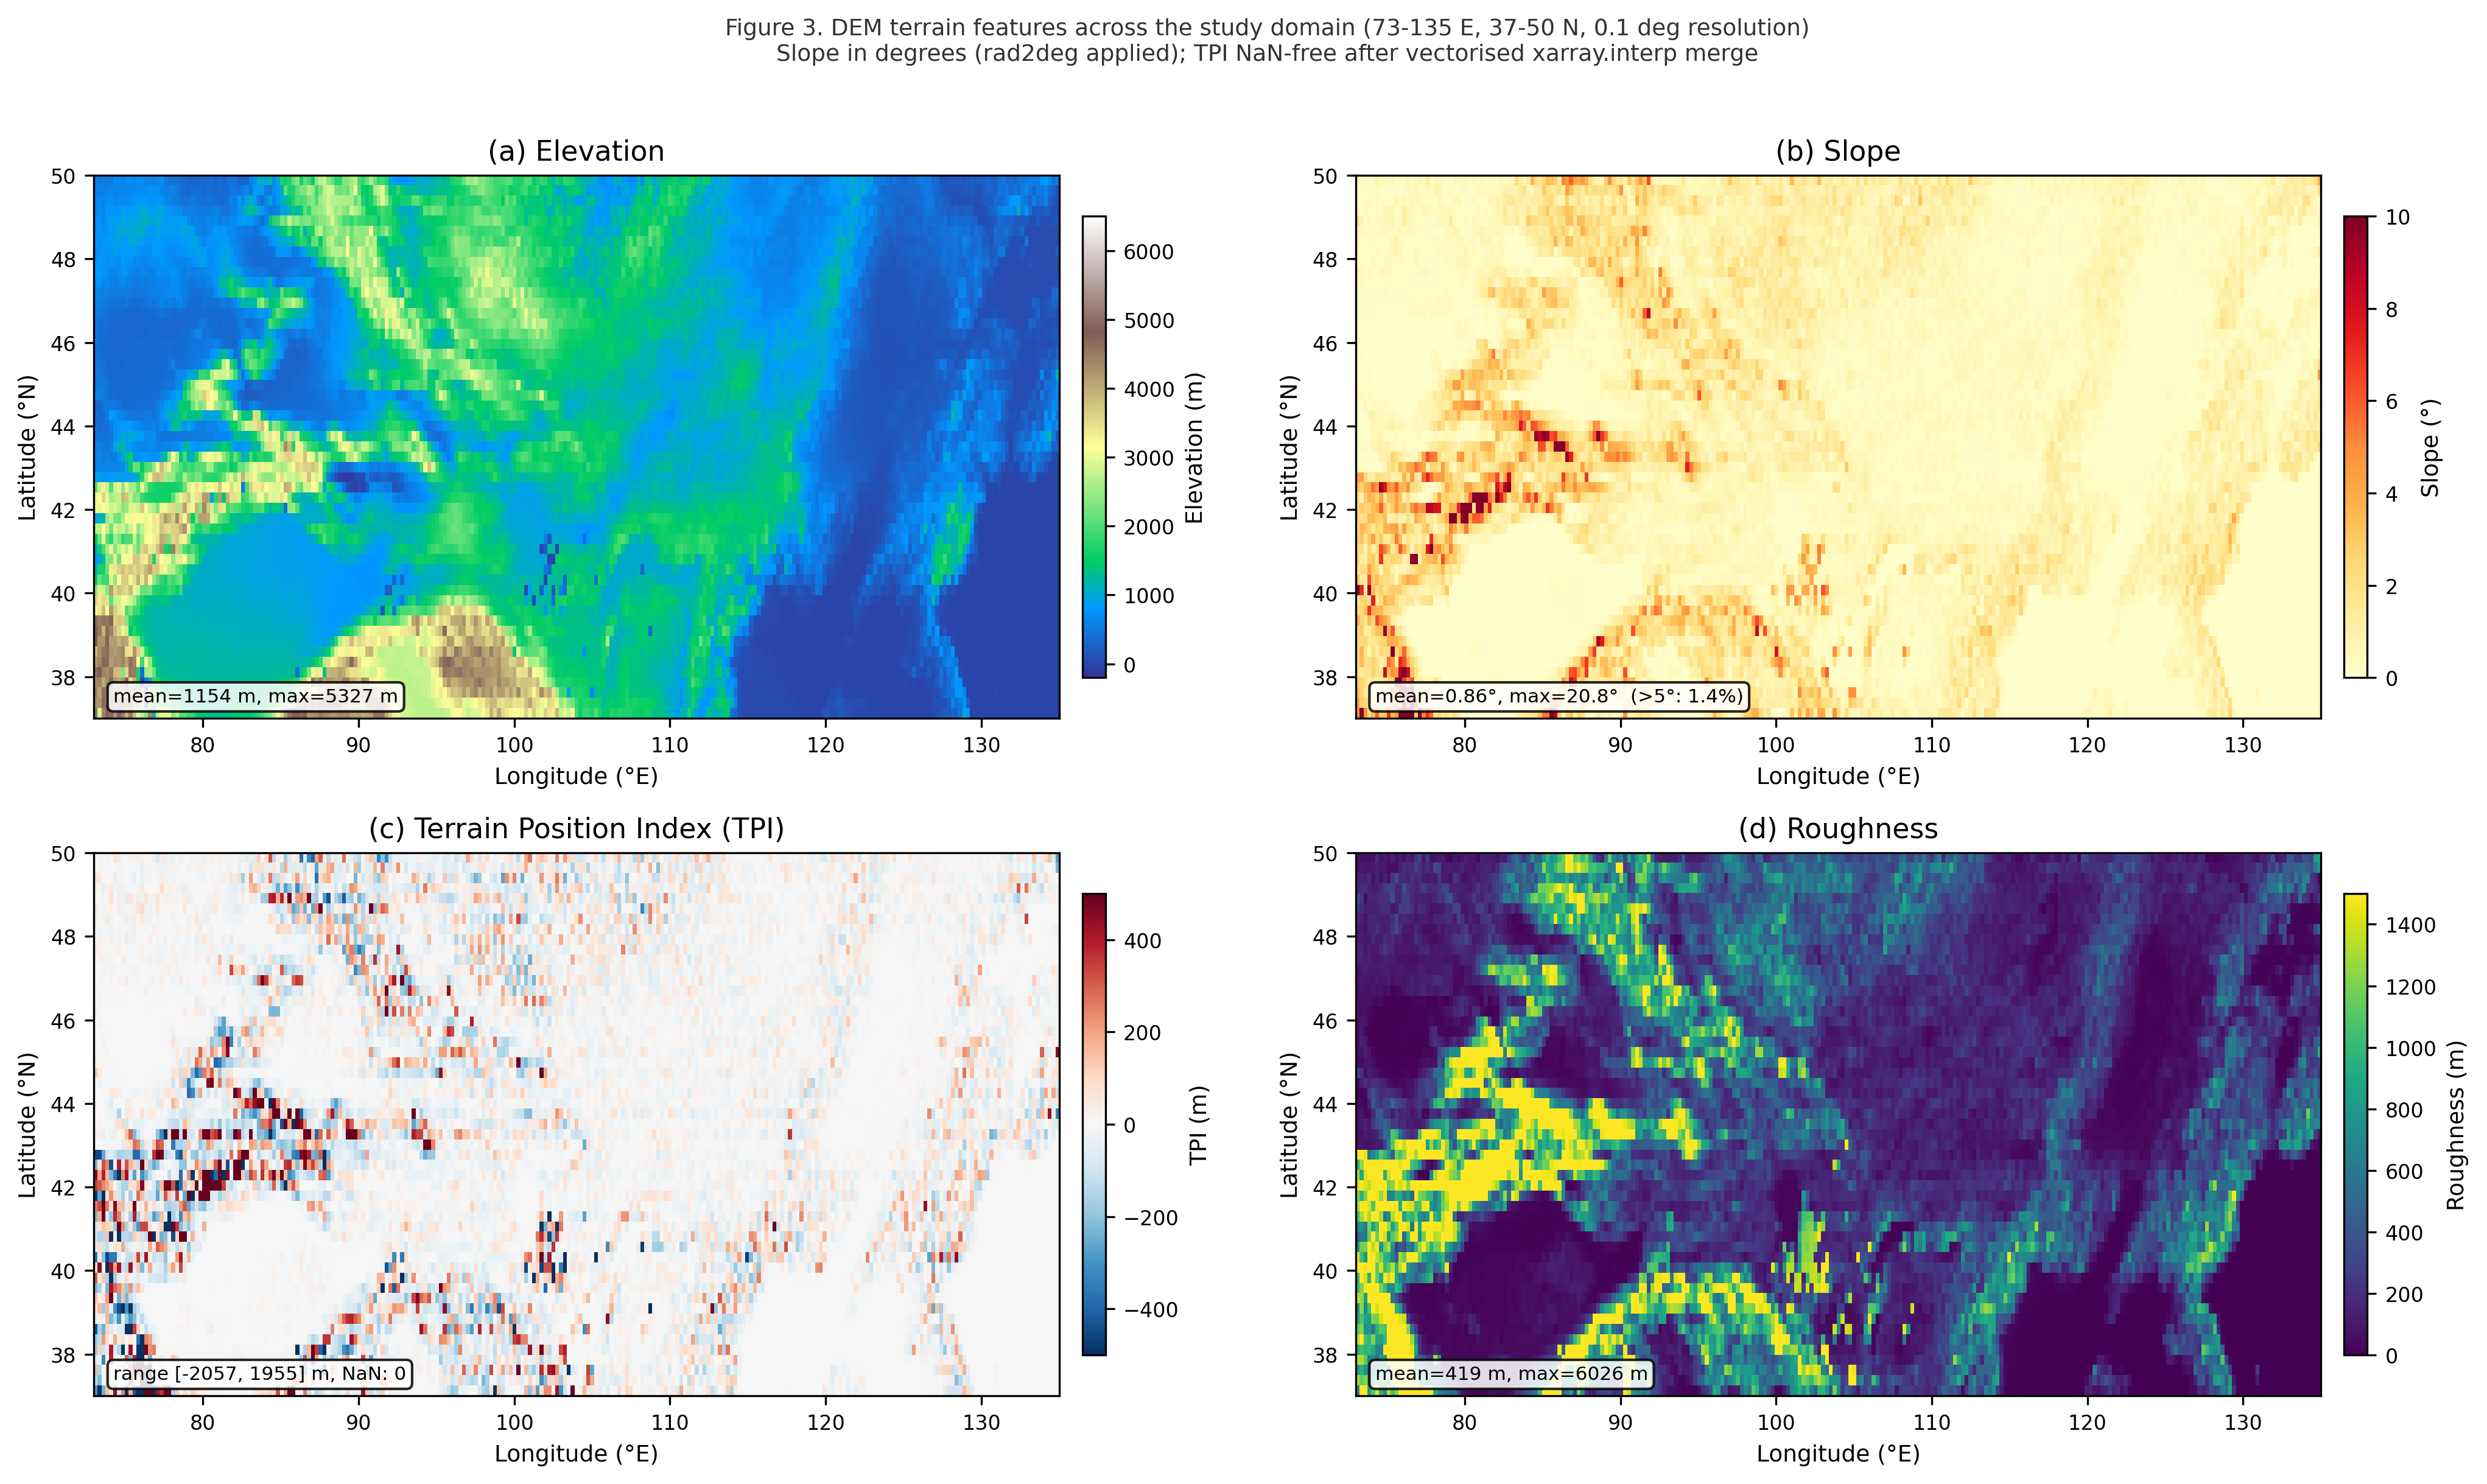
\includegraphics[width=0.95\textwidth]{figure3_terrain_features.png}
\caption{研究区域DEM地形特征}
\label{fig:terrain}
\end{figure}

\subsection{工程与OSM特征}

从OpenStreetMap~\cite{osm2023}提取3个工程可及性特征：到最近输电线路
距离、到最近道路距离和到最近居民点距离，三者共同反映电网接入成本、
施工可达性和社会影响约束。在此基础上，综合上述距离特征构建LCOE代理
指数作为第16个特征，用于近似表征场址的平准化度电成本。距离输电线路
越近、地形坡度越小、距道路越近，LCOE代理值越低，对应更优的工程
可行性。

\subsection{政策语料库}

本研究收集了81份风电及可再生能源政策文件，包括67份国家级文件及
新疆、内蒙古、甘肃、吉林、宁夏、山东六个重点省份的省级规划文件
14份，时间跨度为2002至2026年。国家级文件经人工标注得到1400个句子，
分布为中性471句、鼓励553句、限制251句、禁止125句，标注者间一致性
$\kappa=0.81$；省级文件经规则标注新增12759个句子，合并后语料库共
16433句。省级文件以鼓励类条款为主，各省鼓励比例存在显著差异，
从高到低依次为：宁夏5.0\%、内蒙古4.7\%、甘肃4.1\%、山东2.3\%、
吉林1.4\%、新疆0.6\%，为模型提供了省际政策强度的差异化信号，
弥补了仅依赖国家级文件时各省共享相同政策向量的不足。

图~\ref{fig:policy}展示政策语料库的年度趋势，包括各年度文件数量、
鼓励区域与禁止区域关键词频次对比、技术规范频次以及装机容量目标
数量的历年变化。尽管语料库涵盖2002至2026年并包含"十五五"信号，
这并不构成对2019至2020年验证数据的时间泄漏："十五五"规划延续并
正式化了三北大基地开发的长期政策轨迹，而这一轨迹在验证场址建设之前
已是既定方向。纳入前瞻性文件反映的是中国风电治理的\textit{连续性}，
而非事后信息的引入。2010年后并网要求和鼓励区域政策显著增加，2022年后
禁止区域条款明显上升，与"十二五"以来三北风电基地大力推进及近年
生态红线管控趋严的政策背景一致。

\begin{figure}[H]
\centering
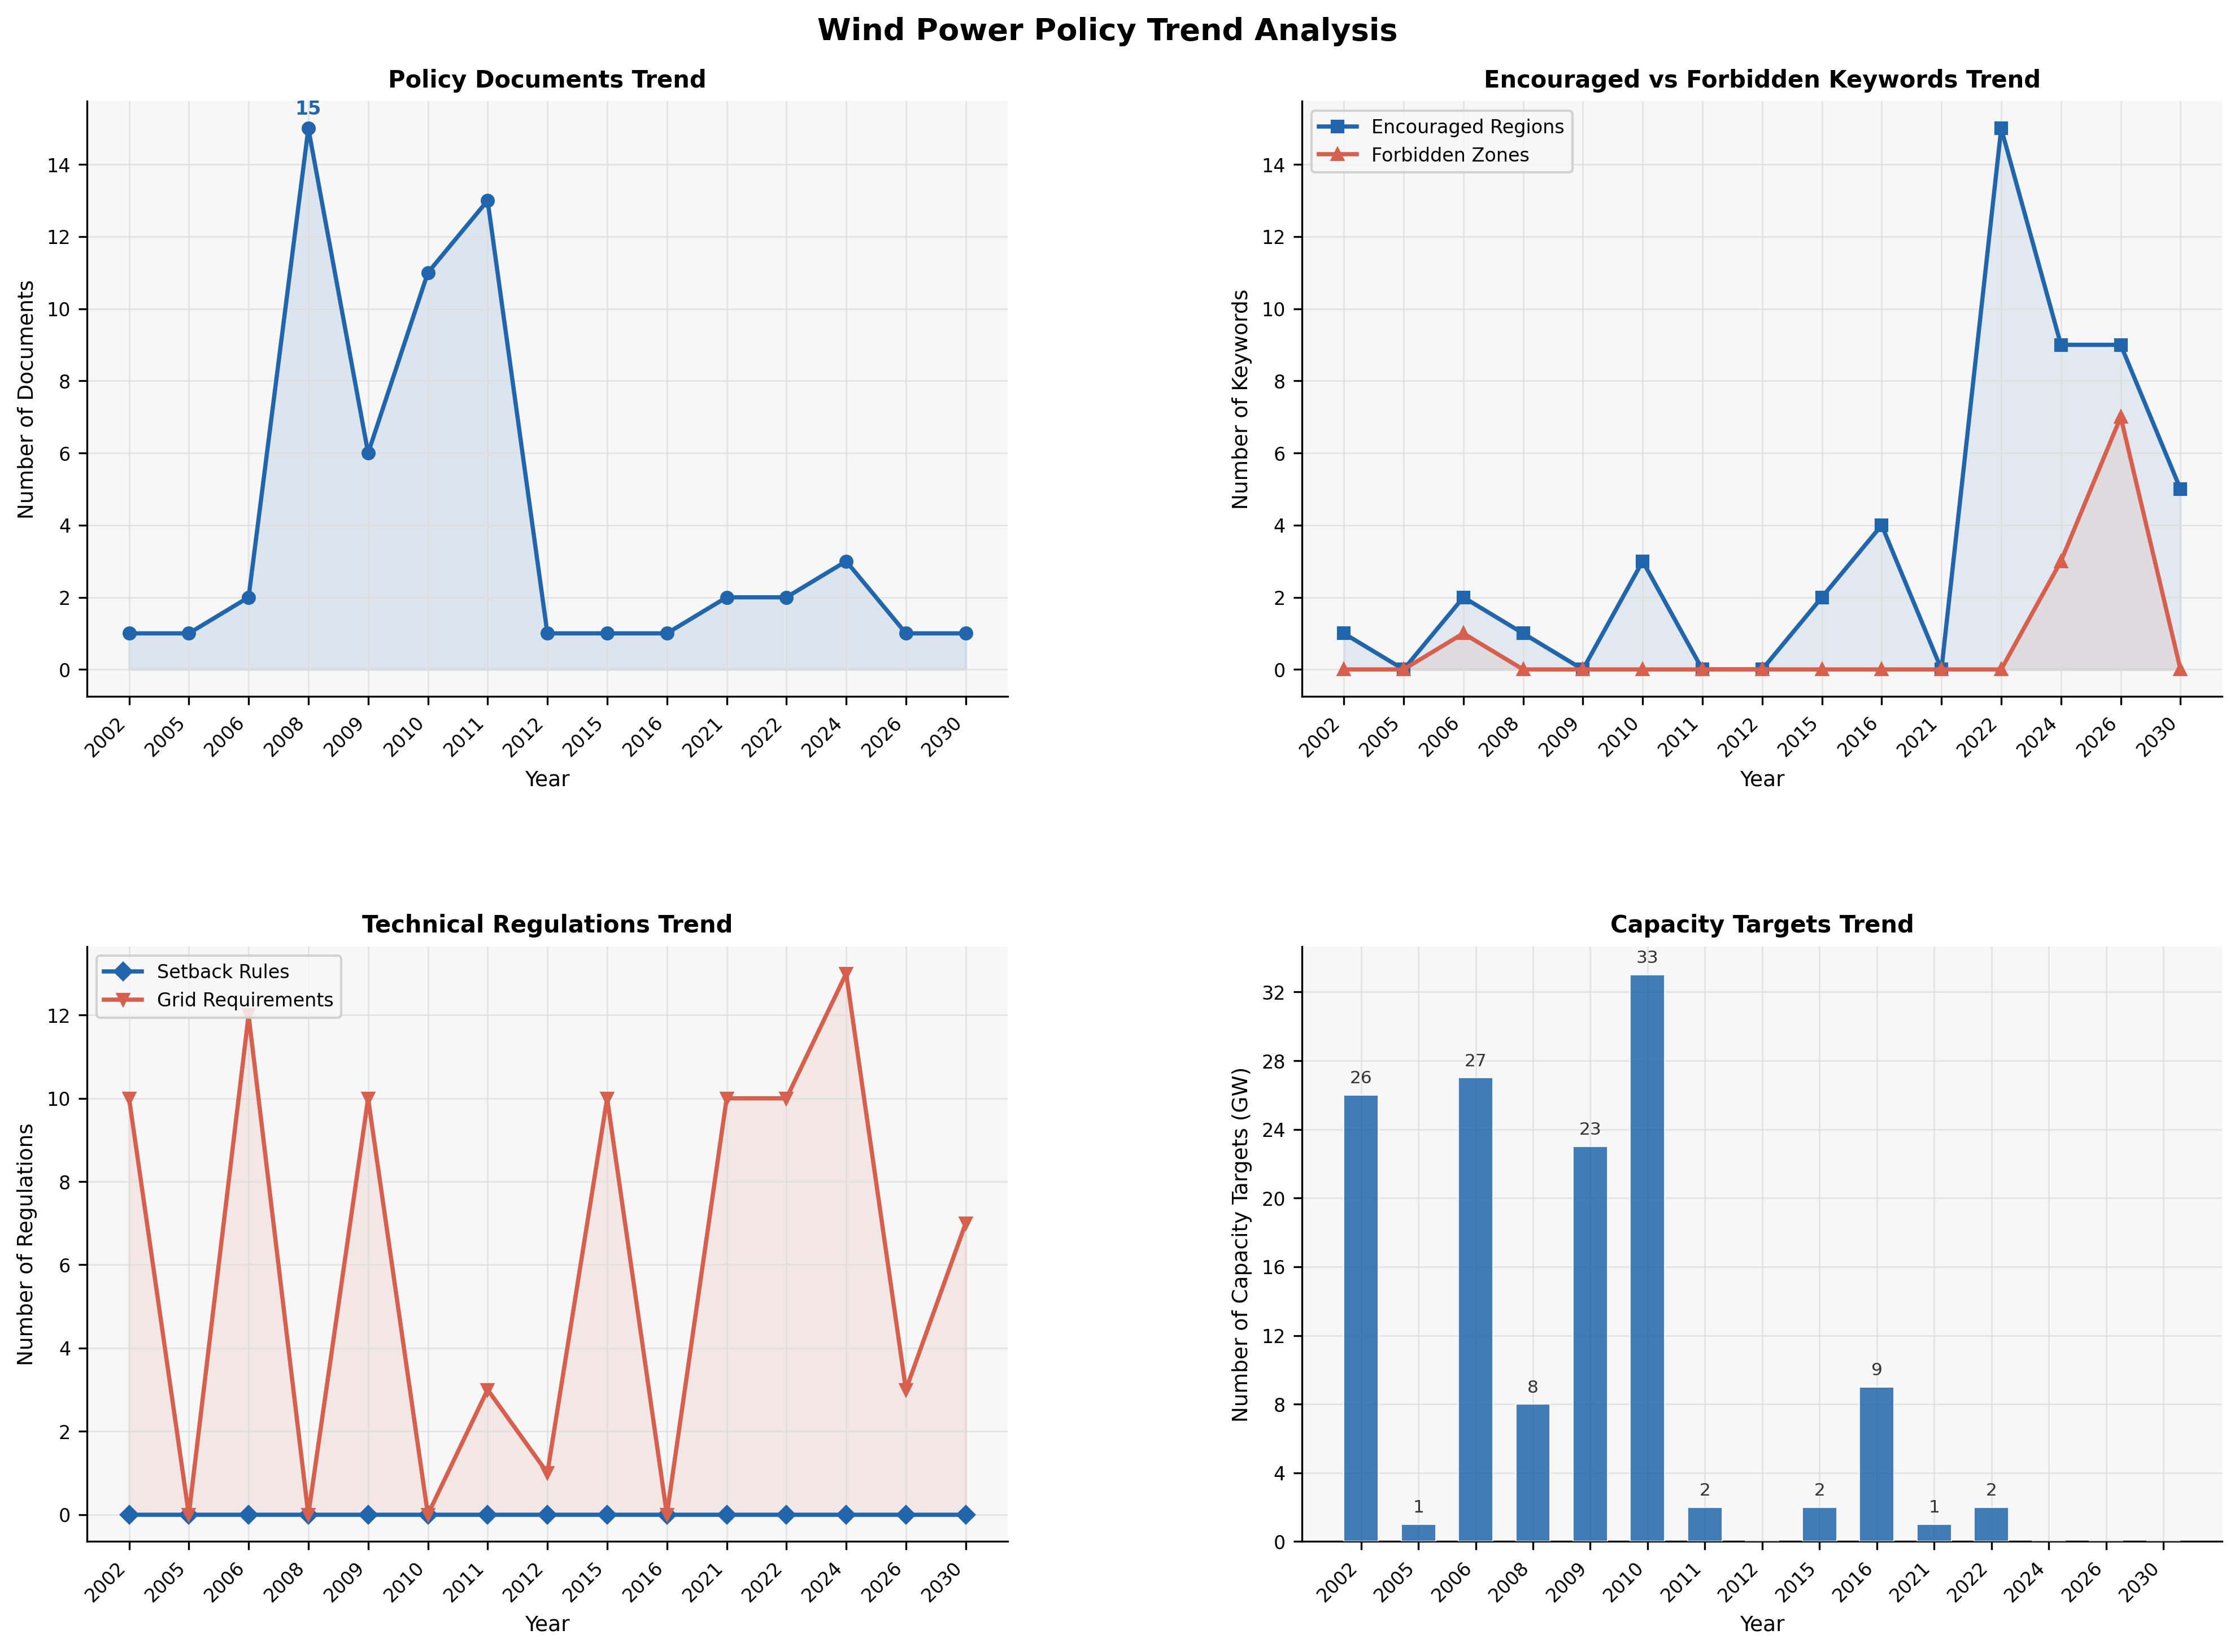
\includegraphics[width=0.95\textwidth]{policy_trend_v2.png}
\caption{中国风电政策语料库年度趋势（2002--2026年）}
\label{fig:policy}
\end{figure}

\subsection{SCADA数据}

九个独立验证风电场总装机约1100\,MW，数据区间为2019至2020年，坐标通过
ERA5相关性匹配推断。图~\ref{fig:samples}以橙色三角形标注789个正样本
（OSM风电场聚类，DBSCAN聚类半径$\varepsilon=3$\,km），蓝色圆点标注
1,578个负样本；九个验证场址以三角形区分置信度：Sites\,1、2、6和7的Pearson相关系数
不低于0.50，置信度较高；Sites\,3、5、8和9相关系数在0.30至0.50之间，
置信度中等；Site\,4相关系数为0.240，置信度偏低；喀什场址因相关系数
仅为0.154而排除。九个场址整体均值相关系数$\bar{r}=0.4540$。

\begin{figure}[H]
\centering
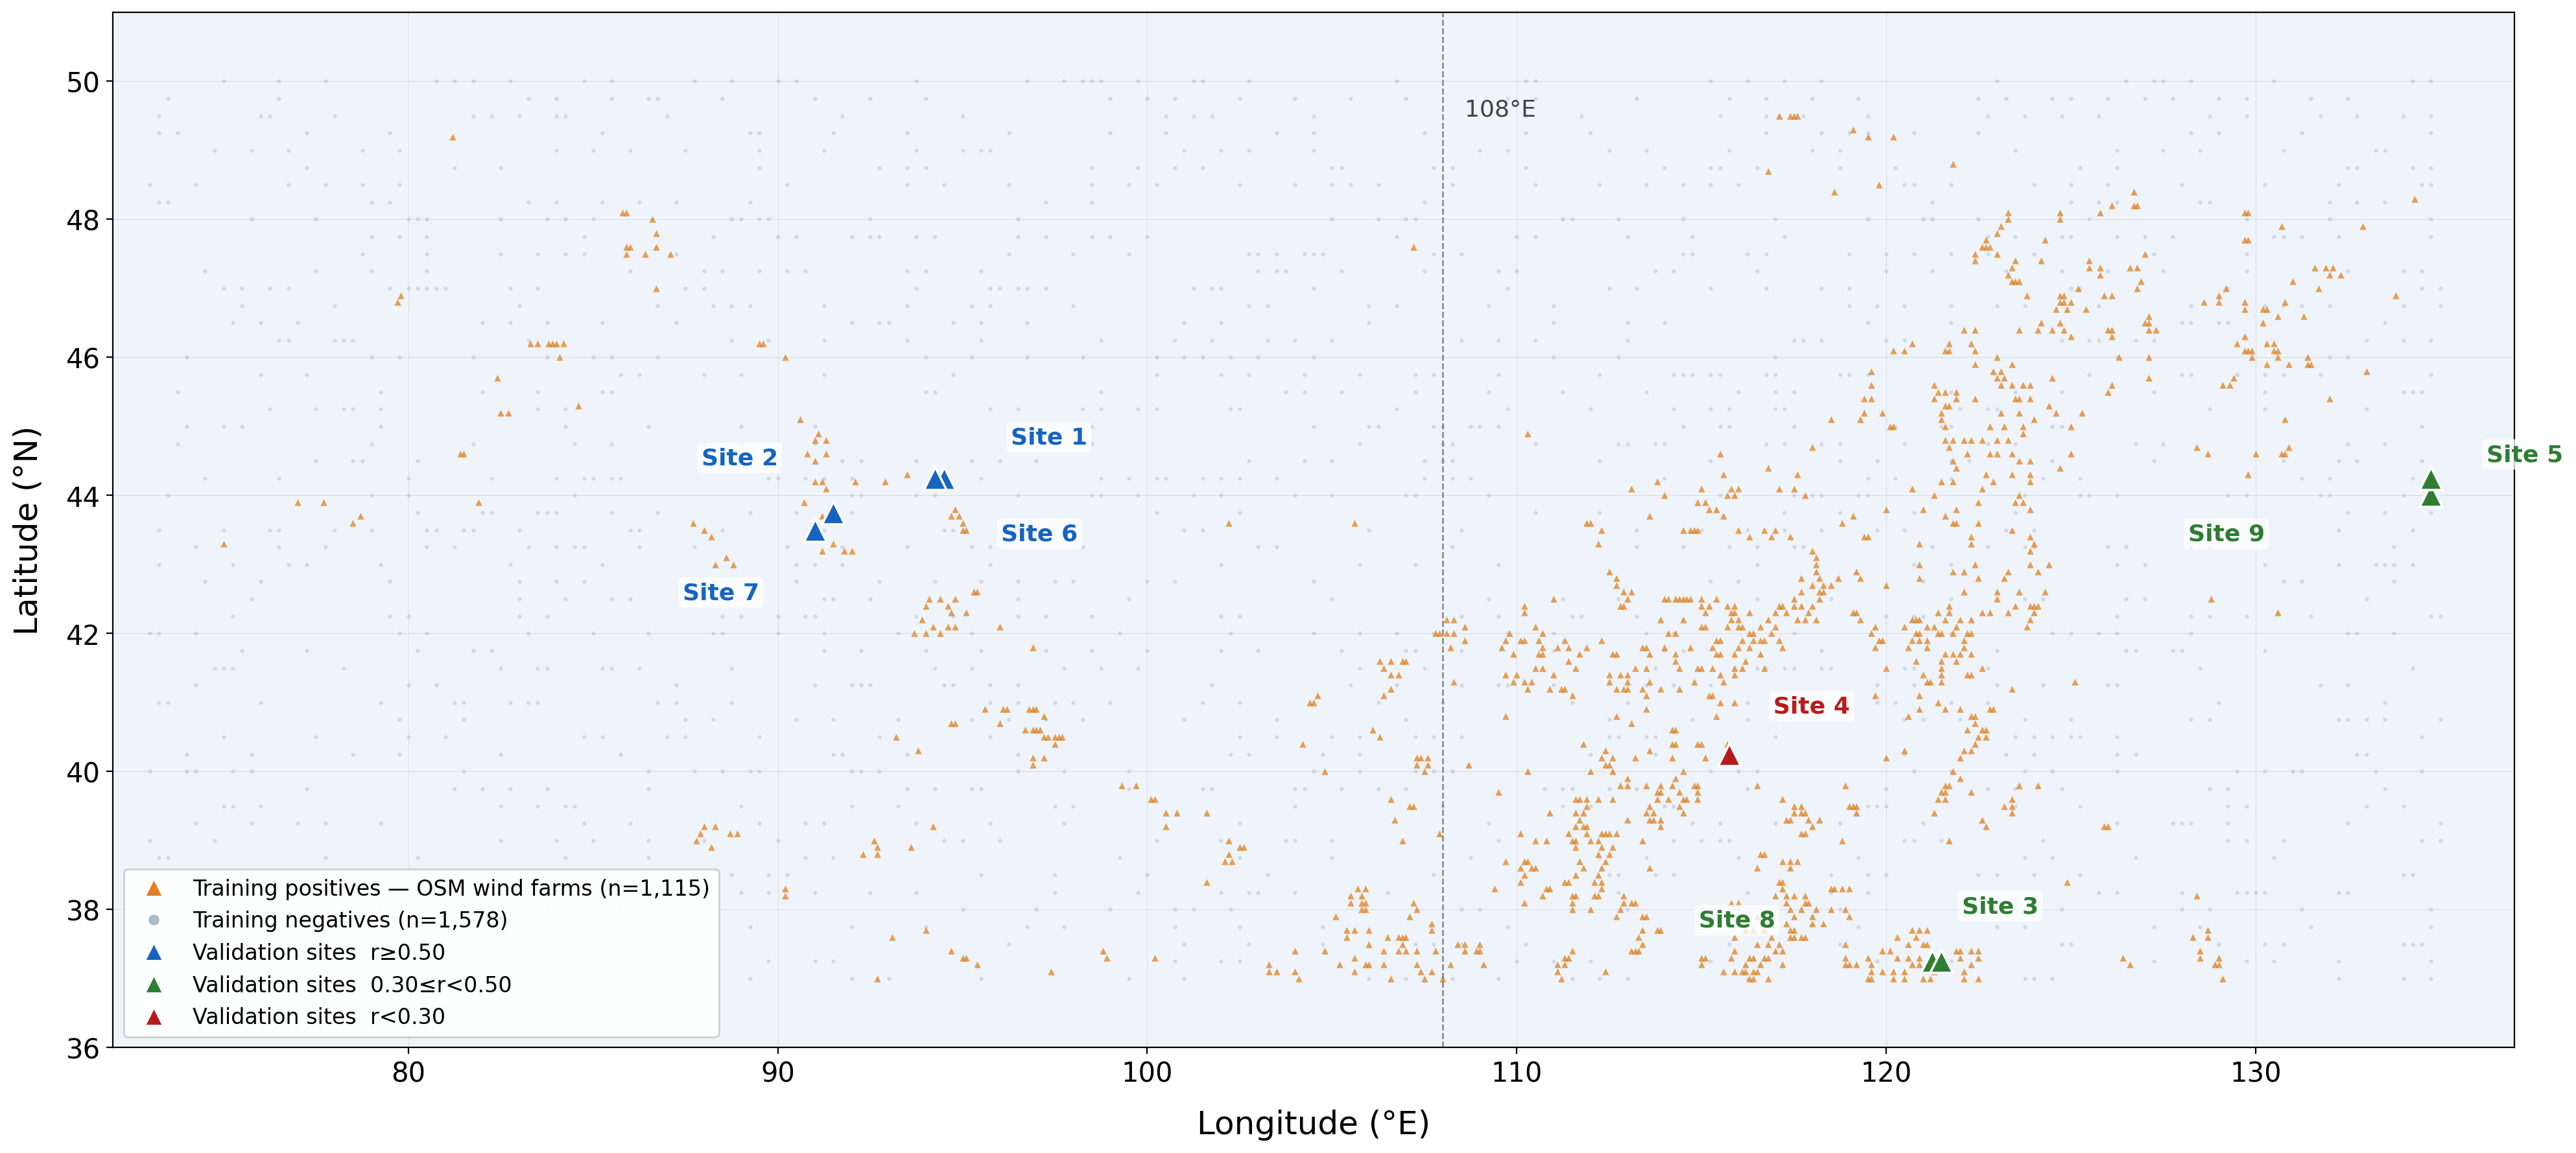
\includegraphics[width=0.95\textwidth]{figure2_training_samples.png}
\caption{训练样本空间分布}
\label{fig:samples}
\end{figure}

% ============================================================
\section{方法}
% ============================================================

本研究提出的双流跨模态融合架构由两条并行编码流、一个跨模态注意力
融合模块和三个多任务输出头构成。数值特征流负责捕捉气象、地形和工程
约束，政策语义流负责将监管文本编码为可与数值特征交互的密集向量，
融合模块通过注意力机制和门控机制将两流自适应结合，输出头则联合优化
三个选址目标。本节依次介绍整体架构、融合模块的数学表达以及训练设置
与评估协议。

\subsection{整体框架}

图~\ref{fig:wind_farm_framework}展示完整的双流架构。左侧蓝色部分为
数值特征流，16个结构化空间特征经TabTransformer编码后输出64维数值
表示向量$\mathbf{F}_\text{num}$；右侧绿色部分为政策语义流，81份政策
文件经BERT+LoRA微调模型编码并映射至13197个格点，输出64维政策语义
向量$\mathbf{F}_\text{policy}$；中央紫色部分为跨模态注意力融合模块，
以$\mathbf{F}_\text{num}$为查询、$\mathbf{F}_\text{policy}$为键和值，
经Sigmoid门控自适应融合后输出64维融合向量$\mathbf{F}_\text{fused}$；
底部橙色部分为三个由GradNorm动态平衡的任务头，分别输出场址适宜性
地图、风资源潜力图和工程适宜性图。

\textbf{数值特征流}负责对16个结构化空间特征进行编码。具体而言，
从2018至2025年100\,m高度ERA5再分析数据提取8个风能特征，包括年均
风速、风速标准差、风功率密度、风速第75百分位数、年均有效发电小时数、
年均高效发电小时数、季节变异系数及风速8年趋势斜率；从0.1$^\circ$
分辨率DEM提取高程、坡度、地形位置指数和粗糙度4个地形特征；从
OpenStreetMap提取到输电线路、道路和居民点的距离3个工程可及性特征，
及综合LCOE代理指数1个特征。上述16个特征经
TabTransformer~\cite{huang2020tabtransformer}编码。

选择TabTransformer的核心动机在于：风电选址的16个数值特征异质性强，
气象、地形、工程量纲差异悬殊，且特征间存在非线性交互，例如坡度与
高程对施工成本具有联合约束效应。TabTransformer通过对每个特征独立
进行可学习线性嵌入后施加Transformer自注意力，能够在不依赖手工特征
工程的条件下自动捕捉跨特征的上下文依赖关系，在此类异质表格数据上的
判别能力显著优于多层感知机~\cite{huang2020tabtransformer}。具体而言，
16个特征经线性嵌入层映射至64维隐空间，经2层、4头自注意力后通过均值
池化输出$\mathbf{F}_\text{num} \in \mathbb{R}^{64}$。注意力头数设为4，
是在模型容量与约2,400个训练样本之间取得平衡，头数过多会导致每头的
子空间维度过小，增加过拟合风险。

\textbf{政策语义流}将非结构化监管文本编码为可与数值特征交互的密集向量。本研究对1400个标注句子采用BERT+LoRA方法进行微调~\cite{devlin2019,hu2022}，
以\texttt{hfl/chinese-roberta-wwm-ext}为预训练底座，在Q和V投影矩阵上注入秩16、缩放因子32的低秩适配矩阵，
测试集宏F1达0.850。相比全量微调，LoRA将可训练参数量压缩至约0.3\%，
在政策语料规模有限的条件下有效抑制了过拟合~\cite{peft2025lora}；
近期基准研究证实，在数据匮乏场景下PEFT是实现稳健泛化的前提条件，
而非仅仅是效率选择。微调后模型对每份文件
生成句子级嵌入并按省级行政边界聚合，最终将13197个ERA5格点映射至
各自所属省份的政策语义向量$\mathbf{F}_\text{policy} \in \mathbb{R}^{64}$。

\textbf{跨模态注意力融合模块}将上述两流输出进行自适应融合。模块采用
4头跨模态注意力，$d_\text{model}=64$，以数值流$\mathbf{F}_\text{num}$
为查询，以政策流$\mathbf{F}_\text{policy}$同时作为键和值，使每个空间
格点的数值表示能主动检索当地监管语义；残差连接后输出
$\mathbf{F}_\text{cross} \in \mathbb{R}^{64}$。随后通过Sigmoid门控
对跨模态特征与原始数值特征进行自适应加权融合，得到最终融合向量
$\mathbf{F}_\text{fused} \in \mathbb{R}^{64}$。该向量随后送入三个由
GradNorm动态平衡的任务头~\cite{chen2018gradnorm}，分别联合预测场址
排名分（头I，收敛权重$\lambda_1 \approx 1.53$）、风能潜力分
（头II，$\lambda_2 \approx 0.02$）和工程及政策合规分
（头III，$\lambda_3 \approx 1.45$）。工程及政策合规头的
设计动机之一在于：风电出力的时序平稳性与电网负荷曲线的匹配程度
直接影响并网消纳能力，将输电可达性、地形约束等工程要素纳入独立任务头，
使框架在识别高风速区的同时优先筛选出力平滑、并网友好的候选场址。

\begin{figure}[H]
\centering
\includegraphics[width=\textwidth]{export.jpg}
\caption{双流跨模态融合架构}
\label{fig:wind_farm_framework}
\end{figure}

\subsection{坐标推断与验证指标}

验证场址坐标通过Pearson相关系数推断，计算各场址月均实测功率
$P_t$与ERA5 100\,m格点风速$W_t$的时序相关：
\begin{equation}
r = \frac{\displaystyle\sum_{t=1}^{T}(P_t - \bar{P})(W_t - \bar{W})}
    {\sqrt{\displaystyle\sum_{t=1}^{T}(P_t-\bar{P})^2
     \cdot\sum_{t=1}^{T}(W_t-\bar{W})^2}}
\label{eq:pearson}
\end{equation}

Weibull分布参数$k$和$c$由极大似然估计从ERA5风速时序拟合：
\begin{equation}
f(v;k,c) = \frac{k}{c}\left(\frac{v}{c}\right)^{k-1}
\exp\!\left[-\left(\frac{v}{c}\right)^k\right], \quad v\geq0
\label{eq:weibull}
\end{equation}
$k$值越高表示风速分布越集中、湍流强度越低，是风电场长期稳定性的
核心代理指标~\cite{jung2021}。LCOE代理指数综合电网距离$d_g$、
道路距离$d_r$和地形坡度$s$：
\begin{equation}
\text{LCOE}_{\text{proxy}} = w_1\,d_g + w_2\,d_r + w_3\,s
\label{eq:lcoe}
\end{equation}
权重$w_1,w_2,w_3$在训练集上以网格搜索标定，使LCOE代理与
风电场开发成本的文献估算相关系数最大化，与国家标准~\cite{gbt19963}
规定的并网成本结构相一致。

\subsection{跨模态注意力融合}

跨模态注意力的计算如下：
\begin{equation}
\mathbf{F}_\text{attn} =
  \text{softmax}\!\left(\frac{\mathbf{Q}\mathbf{K}^\top}{\sqrt{d_k}}
  \right)\mathbf{V},
\quad
\mathbf{Q}=\mathbf{F}_\text{num}\mathbf{W}_Q,
\quad
\mathbf{K}=\mathbf{V}=\mathbf{F}_\text{policy}\mathbf{W}_K
\label{eq:cross_attn}
\end{equation}

将数值流设为查询、政策流设为键与值的设计动机如下：对于给定格点，
模型需要根据该格点自身的气象与工程属性主动检索当地最相关的政策语义，
即哪些监管意图对该类型格点影响最大。若将政策流设为查询，则模型将
被迫用抽象的省级监管向量去检索具体的数值特征，这在物理上是不自然的，
且会损失注意力得分的空间可解释性。缩放因子$d_k=64/4=16$确保注意力
得分方差在合理范围内，避免softmax饱和。

Sigmoid门控融合如下：
\begin{equation}
\mathbf{F}_\text{fused} =
  g \odot \mathbf{F}_\text{attn} +
  (1-g) \odot \mathbf{F}_\text{num},
\quad
g=\sigma\!\left(\mathbf{W}_g[\mathbf{F}_\text{attn};
\mathbf{F}_\text{num}]\right)
\label{eq:gating}
\end{equation}

门控向量$g \in (0,1)^{64}$的物理意义是：对融合表示的每个维度，模型
自适应地决定从跨模态注意力输出中吸收多少信息，以及保留多少原始数值
表示。相比简单加权平均或拼接后线性变换，Sigmoid门控的非线性使模型
能够对政策影响较弱的区域自动降低$g$值，对政策约束复杂的区域提升
$g$值，从而实现空间自适应的双流融合~\cite{qiu2025gated}。

\subsection{训练设置与四实验体系}
\label{sec:training}

\textbf{数据划分。}
省级分层划分（以下简称PSS协议）按内蒙古、新疆、甘肃、黑龙江、山东、吉林、宁夏、河北、
辽宁、陕西10个代表性省份对1115个OSM正样本进行均衡分层，划分为
训练集2367个，其中正样本789个；验证集489个，其中正样本163个；
测试集489个，其中正样本163个；确保每个省份在三个子集中均有代表性
覆盖。

\textbf{优化器与学习率。}
采用AdamW优化器~\cite{loshchilov2019}，学习率$3\times10^{-4}$，
权重衰减$1\times10^{-4}$。AdamW将权重衰减从梯度更新中解耦，
在Transformer类架构上具有更好的正则化效果~\cite{loshchilov2019}。
最多训练400轮，以验证集AUC为早停监控指标，耐心值设为50轮，
在第150轮达到最优检查点（AUC=0.9983，第200轮触发早停。

\textbf{GradNorm超参数。}
GradNorm~\cite{chen2018gradnorm}通过动态调整各任务损失权重$\lambda_i$，
使各任务的梯度范数趋近目标比率：
\begin{equation}
\mathcal{L}_{\text{GradNorm}} = \sum_{i=1}^{3}
\left|\,G_i(t) - \bar{G}(t)\cdot r_i^\alpha\,\right|_1
\label{eq:gradnorm}
\end{equation}
其中$G_i(t)$为第$i$个任务头在$t$步的梯度范数，$\bar{G}(t)$为均值，
$r_i$为任务$i$的相对训练速率，$\alpha=1.5$控制收敛速率。
任务平衡超参数$\alpha=1.5$，
控制任务损失梯度范数趋近目标比率的速率；收敛后三任务权重稳定在
$\lambda_1\approx1.53$、$\lambda_2\approx0.02$、$\lambda_3\approx1.45$，
反映场址排名与工程合规任务的联合主导地位。$\lambda_2$极小反映风资源
任务的梯度范数在三任务中最小，即该任务在当前数据集上已接近收敛，
GradNorm自适应地将优化资源分配给更难收敛的另外两个任务，并不意味着
风资源任务被忽略。

表~\ref{tab:exps}汇总四套实验评估协议，不同划分策略对应不同的泛化性
测试目标。需要说明实验四与PSS基准的关系：两者使用相同的OSM正样本与PSS
省级分层划分，区别仅在于评估协议。实验四固定单次随机种子，专用于消融
分析和SHAP计算，所报AUC为0.9650，为单次运行结果；PSS基准采用多轮训练
并取最优检查点，所报AUC为0.9950，为该协议下的最优性能。两个数值反映
同一数据集在不同评估设置下的结果，并非来自不同数据集，直接比较时
需注意这一前提。

\begin{table}[H]
\centering
\caption{四套实验评估体系对比（所有实验使用相同训练权重）}
\label{tab:exps}
\small
\begin{tabularx}{\textwidth}{clXllX}
\toprule
\textbf{实验} & \textbf{正样本来源} & \textbf{划分策略} &
\textbf{特征} & \textbf{AUC} & \textbf{主要目的} \\
\midrule
1 & 9个独立场址 & 独立空间留出 & 数值+政策 &
  \textbf{0.8970} & 真实泛化性 \\
2 & OSM 1115个 & 严格东西向（108$^\circ$E） & 数值+政策 &
  \textbf{0.6710} & 地理泛化能力 \\
3 & OSM 1115个 & 省级分层（PSS） & 仅数值 &
  0.8820 & 政策流消融基线 \\
4 & OSM 1115个 & 省级分层（PSS） & 数值+政策 &
  0.9650 & 消融与SHAP分析 \\
PSS & OSM 1115个 & 均衡分层（10省） & 数值+政策 &
  \textbf{0.9950} & 方法横向对比 \\
\bottomrule
\end{tabularx}
\end{table}

% ============================================================
\section{结果}
\label{sec:results}
% ============================================================

本节依次呈现训练动态、模型性能与方法对比、消融实验、SHAP特征重要性
分析、独立SCADA验证以及全国适宜性地图六个方面的结果。总体而言，
模型在省级分层基准上表现最优，在严格地理留出实验中揭示了跨气候带的
泛化局限，消融实验量化了政策流的独立贡献，SCADA验证证实了模型对
真实运行场址的识别能力。

\subsection{训练动态}

图~\ref{fig:training}展示PSS数据集上的训练曲线，训练集2367个样本，
验证集489个样本，早停耐心值50轮。面板a为训练损失曲线：前5轮因
GradNorm初始化快速下降，第20轮权重稳定后趋于收敛，第150轮后进入
早停等待期出现短暂波动。面板b为验证AUC-ROC曲线：训练损失从首轮快速
下降，于第20轮GradNorm稳定后趋于收敛；验证AUC在前30轮快速上升至
0.9900，之后在GradNorm多任务动态加权驱动下出现振荡，最优检查点记录
于第150轮（AUC=0.9983，第200轮触发早停。后期振荡源于多任务损失
地貌特性，而非过拟合所致。

\begin{figure}[H]
\centering
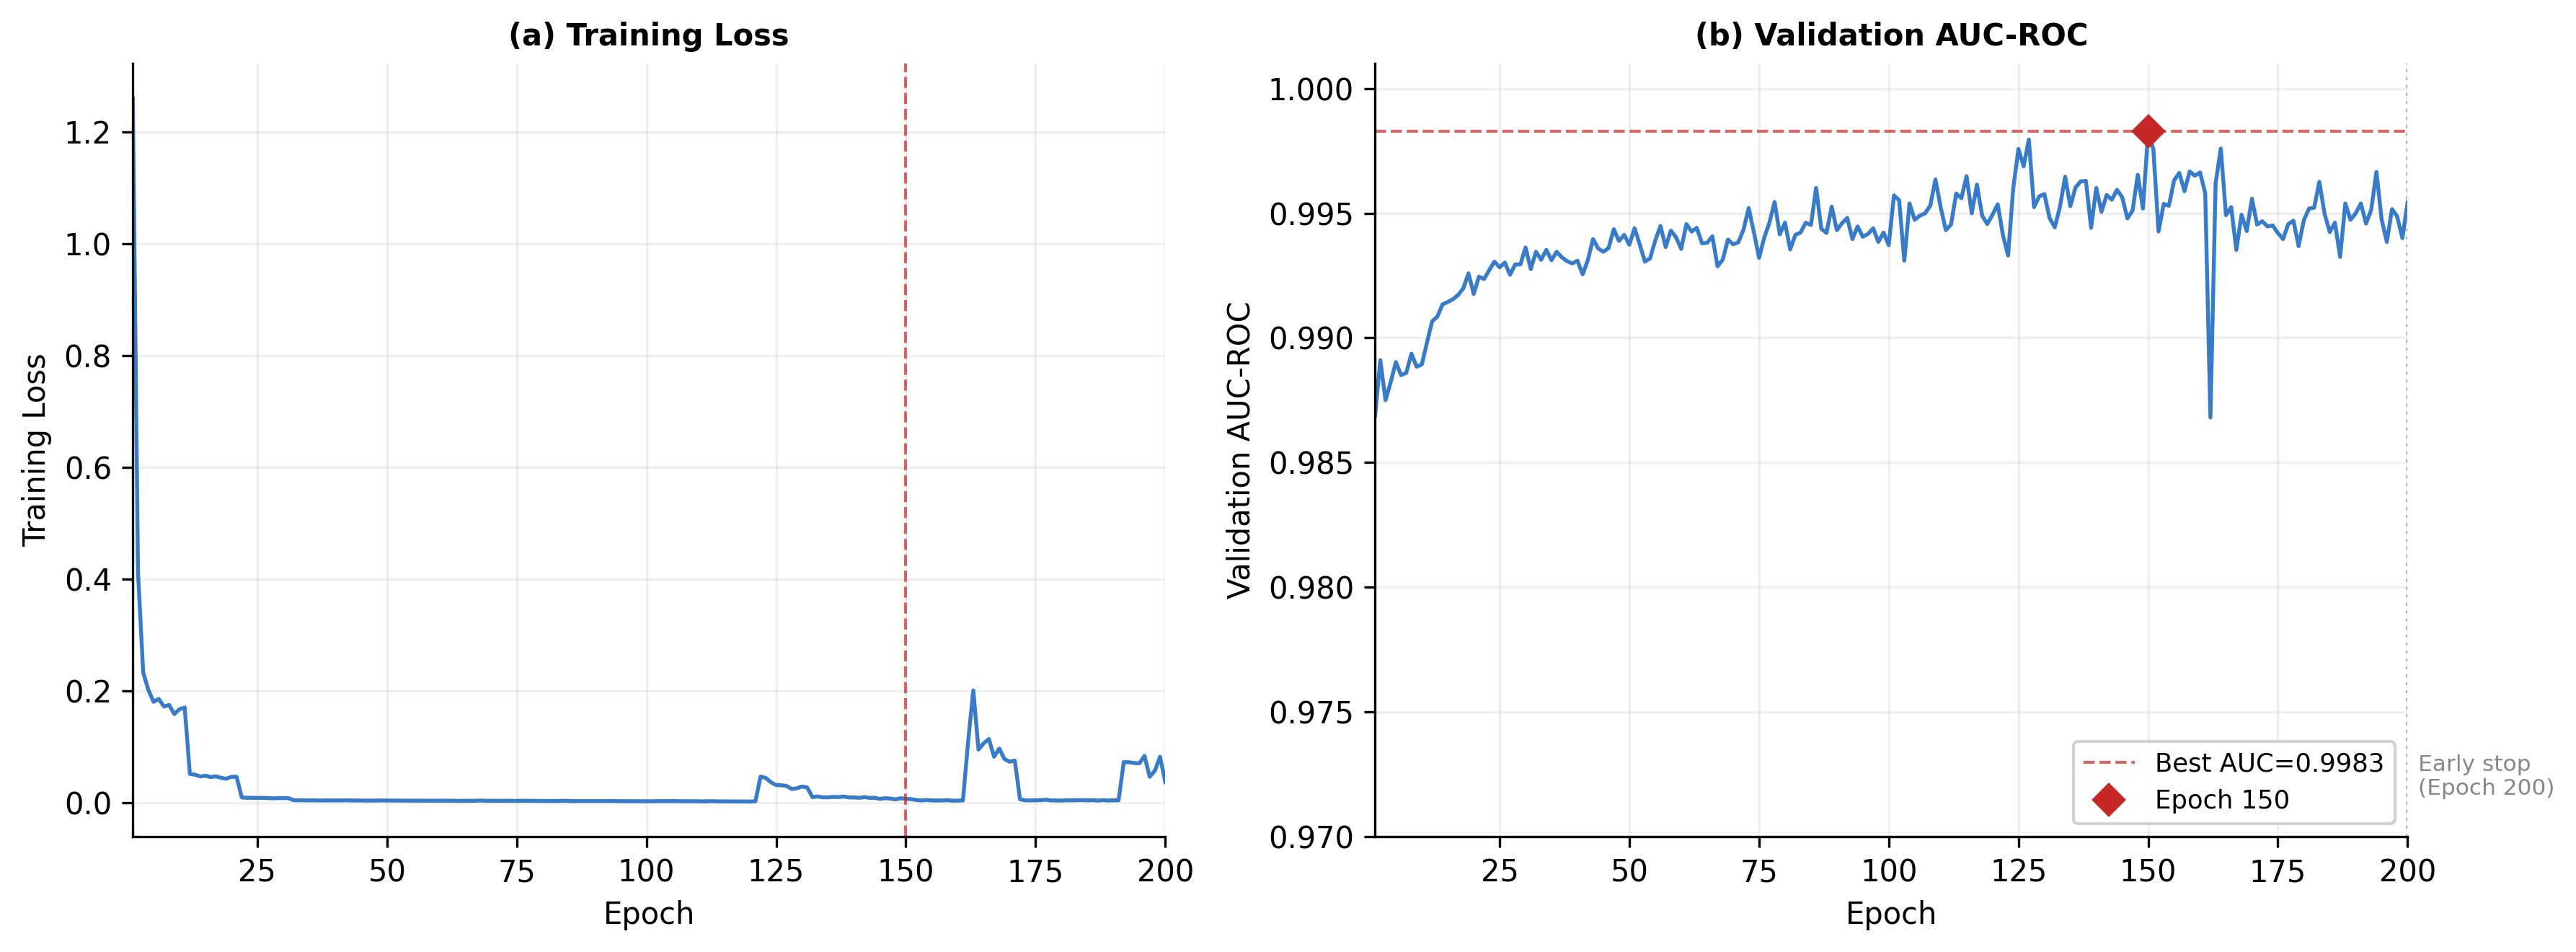
\includegraphics[width=0.95\textwidth]{figure6.png}
\caption{PSS数据集上的训练动态}
\label{fig:training}
\end{figure}

\subsection{模型性能与方法对比}

表~\ref{tab:perf}展示PSS测试集（489个样本，含163个正样本）上的性能
对比。在省级分层基准上，本文框架AUC-ROC达0.9950，Wilcoxon检验显示
与XGBoost的差异具有统计显著性，XGBoost的AUC=0.9900，，$p=0.019$。需要指出的是，
PSS数据集正样本率为33.3\%，各方法AUC均高于0.987，存在天花板效应，
实验四的消融证据更能体现政策流的判别贡献。

\begin{table}[H]
\centering
\caption{PSS评估集上各方法性能对比}
\label{tab:perf}
\small
\begin{tabular}{lcccc}
\toprule
\textbf{方法} & \textbf{AUC-ROC} & \textbf{AP} &
\textbf{Top-163召回} & \textbf{说明} \\
\midrule
随机基线       & 0.5000 & 0.3330 & —     & — \\
AHP$^\dagger$  & 0.6960 & 0.1460 & —     & 实验4测试集 \\
TOPSIS$^\dagger$& 0.6910 & 0.1440 & —    & 实验4测试集 \\
随机森林       & 0.9870 & 0.9790 & 0.9700 & PSS，仅数值 \\
XGBoost        & 0.9900 & 0.9890 & 0.9700 & PSS，仅数值 \\
\textbf{本文（TabTransformer）} &
  \textbf{0.9950} & \textbf{0.9940} & \textbf{0.9750} &
  PSS，数值+政策（81份文件） \\
\midrule
\multicolumn{5}{l}{实验一独立验证（Sites\,1--9）：
  AUC=0.8970，Top-500召回率=0.333，Top-1000召回率=0.444} \\
\multicolumn{5}{l}{实验二东西向留出：AUC=0.6710} \\
\bottomrule
\multicolumn{5}{p{0.9\textwidth}}{\small $^\dagger$
  AHP/TOPSIS在实验4（3300个样本，正样本率9.6\%）上评估，
  与本框架的PSS数据集存在分布差异，直接数值比较仅供参考量级
  判断。PSS测试集正样本率33.3\%（163/489），远高于全国格点尺度的
  真实场址密度（约8.5\%），这一类别比例偏高是各方法AUC集中于
  0.9870至0.9950区间、出现天花板效应的直接原因。政策流的判别贡献
  应以实验四（正样本率9.6\%，更接近真实场景）的消融结果为主要
  参考：在该设置下$\Delta\text{AUC}=+0.0650$，Wilcoxon检验$p=0.019$，
  效应量更具实际意义。}
\end{tabular}
\end{table}

\subsection{消融实验}
\label{sec:ablation}

本研究从两个层面对框架的关键组件进行验证。第一层面为政策语义流的
贡献验证，通过省份哑变量对照实验排除"政策流仅编码省份标签"的竞争性
解释；第二层面为架构设计的合理性支撑，通过SHAP特征重要性分析和
Sigmoid门控值空间分布提供可解释性证据。TabTransformer作为异质数值
特征的上下文编码机制和跨模态注意力作为政策语义动态查询机制，其架构
选择依据领域知识驱动的设计动机，相关可解释性证据见第~\ref{sec:shap}节
和第~\ref{sec:gating}节。

在实验二数据集上，去除政策流后均值AUC从0.7640降至0.6590，
降幅为0.1050，Wilcoxon检验$p=0.002$，证实跨模态注意力模块确实
主动利用了政策嵌入的语义信息。

为排除"政策流仅编码省份标签而非语义内容"的竞争性解释，本研究在
实验二数据集（东西向严格留出，115$^\circ$E分割）上引入两个对照变体：
V6以可学习省份嵌入替代BERT+LoRA编码器，嵌入维度为64维且参与梯度更新，
V7以随机冻结省份嵌入作为零假设基线。在V3基线AUC为0.65900的基础上，
三者与完整模型V5的对比见表~\ref{tab:ablation_policy}。

图~\ref{fig:ablation_policy}展示四个变体在10个随机种子下的AUC-ROC
和平均精度，误差棒表示一个标准差范围。结果呈现清晰的层次递进关系：
V3小于V6小于V5，且每步提升均具有统计显著性。V7（随机嵌入，
AUC=0.6670）与V3无显著差异，证明嵌入维度本身不产生贡献；V6显著
优于V3，Wilcoxon检验$p=0.014$，说明省份信息对跨区泛化具有独立贡献；
V5进一步显著优于V6，Wilcoxon检验$p=0.002$，增量
$\Delta\text{AUC}=+0.0790$，证明BERT+LoRA编码的
监管语义在控制省份信息后仍提供不可替代的增量判别贡献，政策流的
作用不可被省份哑变量解释。

\begin{table}[H]
\centering
\caption{政策流省份哑变量对照实验（实验二数据集，
10个随机种子，均值$\pm$标准差）}
\label{tab:ablation_policy}
\small
\begin{tabular}{llcc}
\toprule
\textbf{变体} & \textbf{政策流内容} &
\textbf{AUC-ROC} & \textbf{AP} \\
\midrule
V3 & 无政策流（数值基线） &
  $0.6590\pm0.0220$ & $0.5340\pm0.0250$ \\
V7 & 随机省份嵌入（零假设） &
  $0.6670\pm0.0210$ & $0.5300\pm0.0180$ \\
V6 & 可学习省份嵌入（关键对照） &
  $0.6850\pm0.0150$ & $0.5770\pm0.0230$ \\
\textbf{V5} & \textbf{完整BERT+LoRA} &
  $\mathbf{0.7640\pm0.0160}$ & $\mathbf{0.7000\pm0.0140}$ \\
\bottomrule
\multicolumn{4}{p{0.85\textwidth}}{\small
  Wilcoxon符号秩检验：V5 vs.\ V6，$p=0.002$；
  V6 vs.\ V3，$p=0.014$；V5 vs.\ V3，$p=0.002$。
  所有对比均在$\alpha=0.05$水平显著。} \\
\end{tabular}
\end{table}

\begin{figure}[H]
\centering
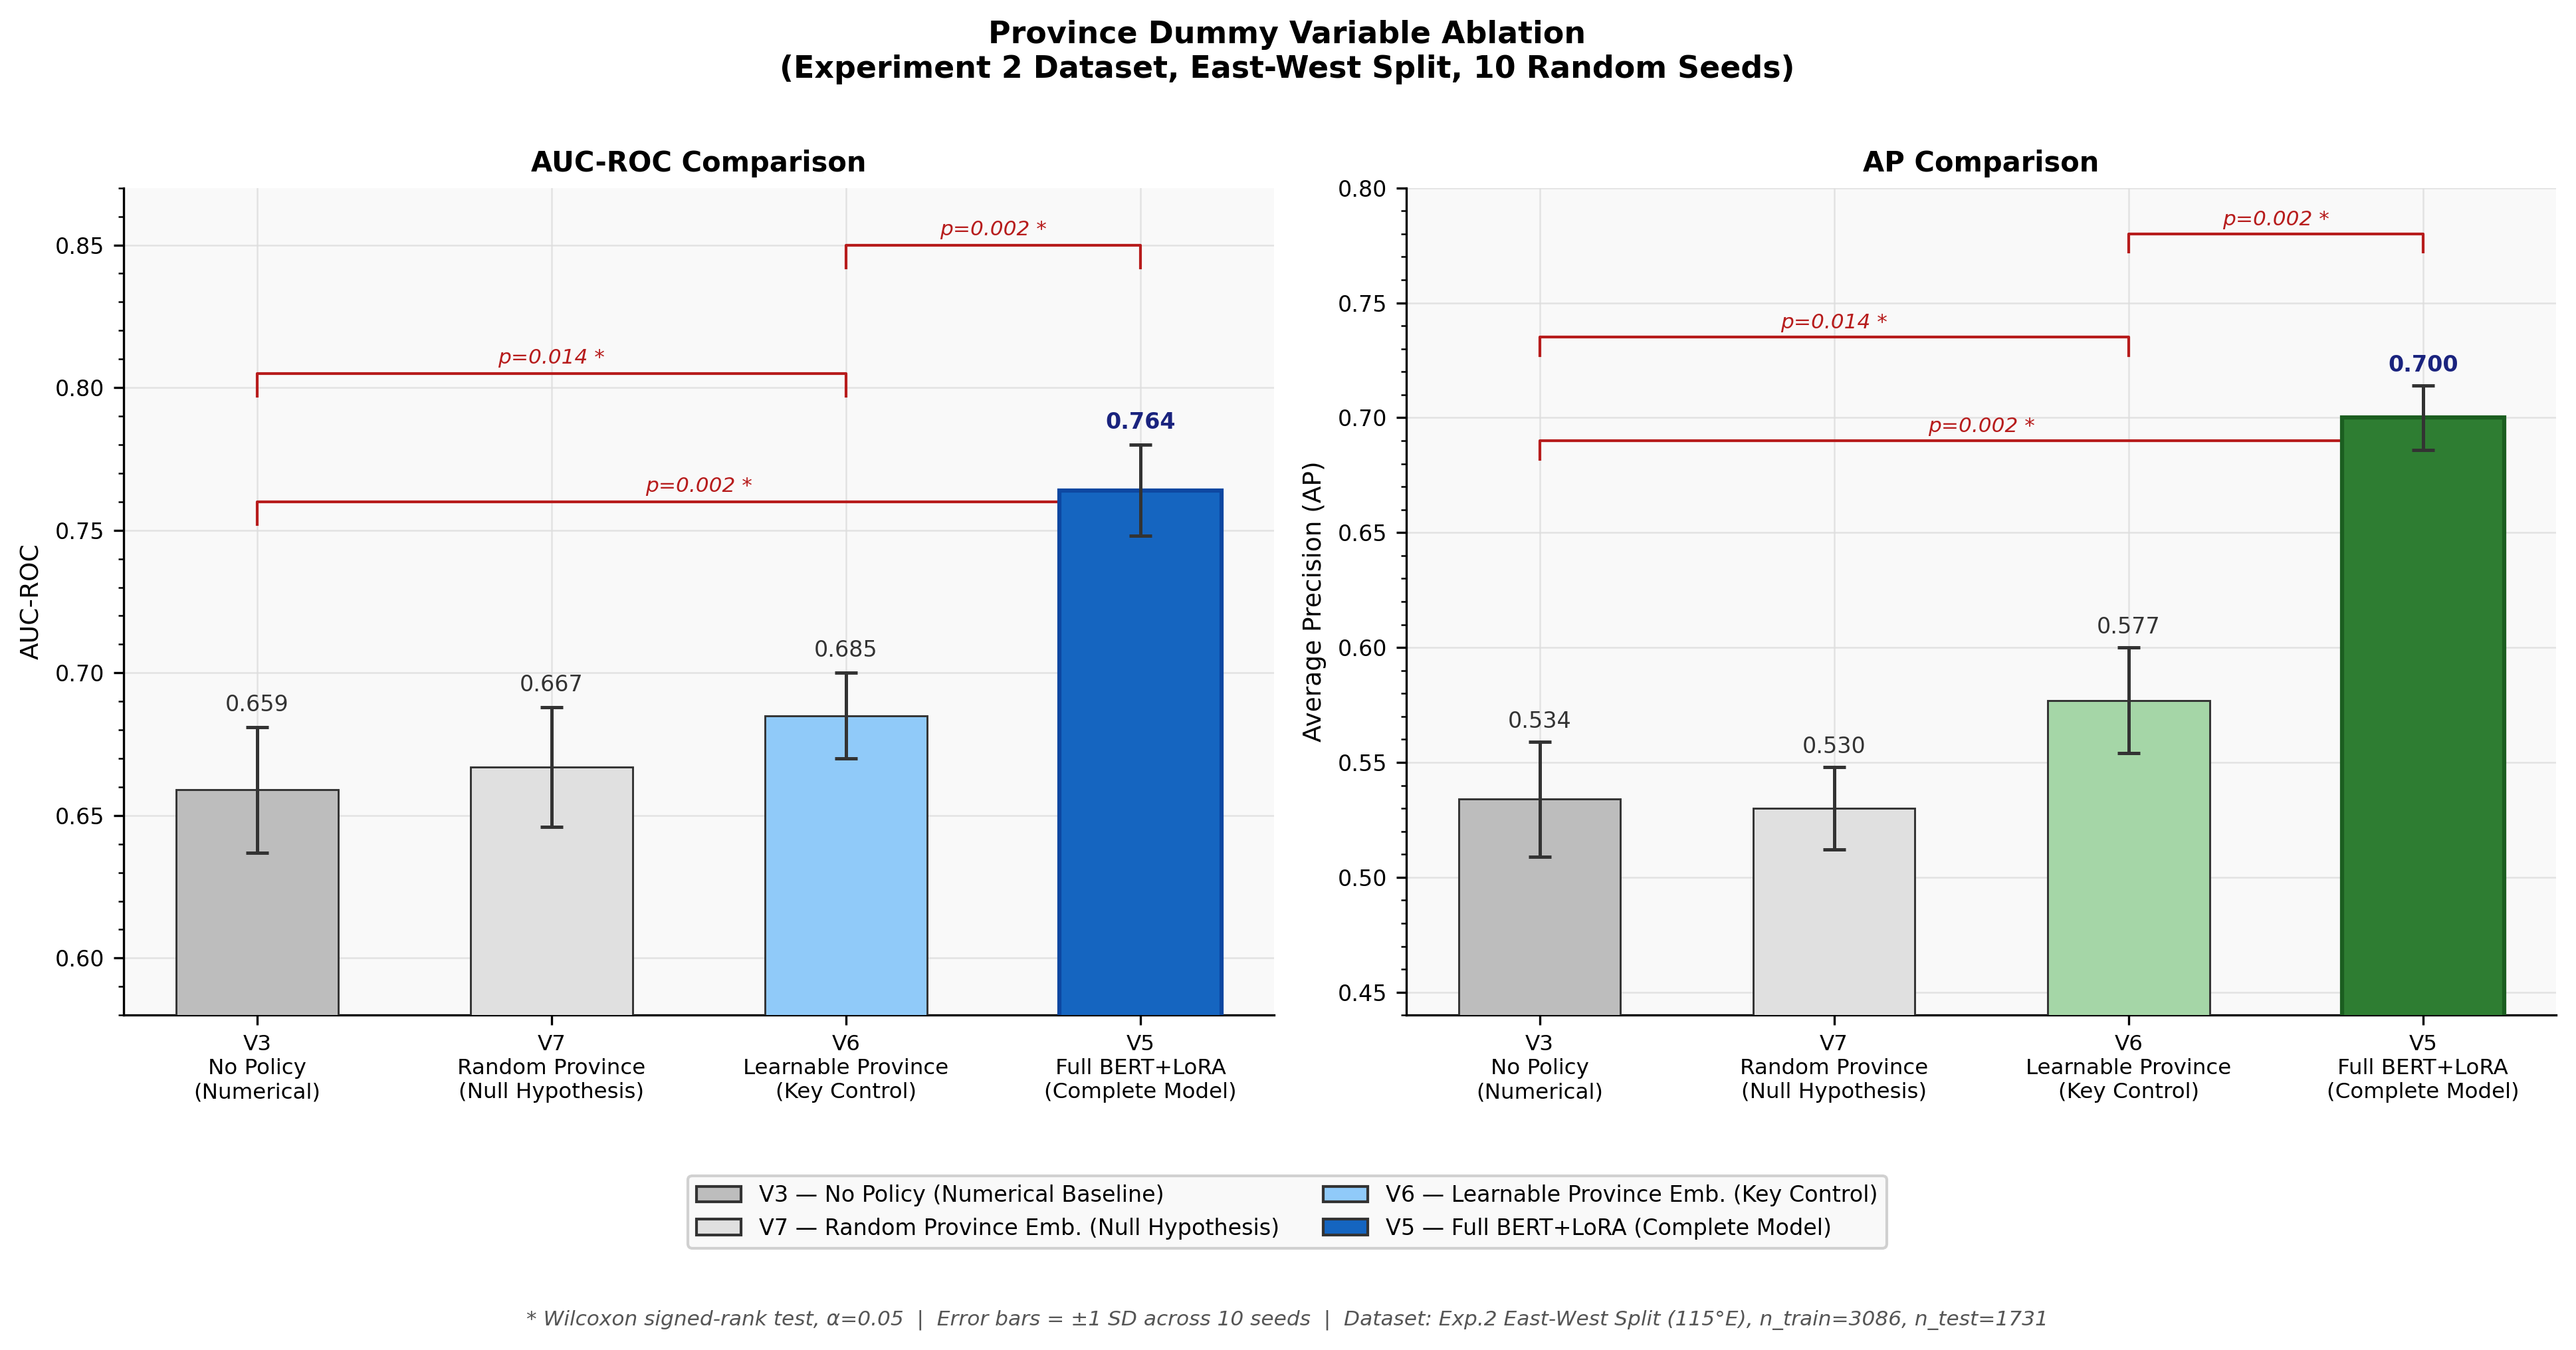
\includegraphics[width=0.95\textwidth]{ablation_policy_exp2.png}
\caption{政策流省份哑变量对照实验结果}
\label{fig:ablation_policy}
\end{figure}

\subsection{政策语义的跨省迁移性验证：留一省实验}
\label{sec:lopo}

为进一步验证BERT+LoRA提取的是通用监管逻辑而非行政标签记忆，本研究
引入\textbf{留一省验证（LOPO）}协议：依次剔除一个完整省份的全部格点
进行训练，迫使模型仅凭政策语义对"未见省份"进行选址推理。研究区域
七个省份中正样本达到评估门槛（$\geq3$）的有三个，其余四个因样本不足
跳过，反映了OSM数据高度集中于内蒙古的真实分布。表~\ref{tab:lopo}
对比V5（完整BERT+LoRA）、V6（可学习省份嵌入）与V3（无政策流）。

\begin{table}[H]
\centering
\caption{留一省验证结果与独立场址分布对比（鼓励比例来自
第\ref{sec:policy}节）}
\label{tab:lopo}
\small
\begin{tabular}{lccccc}
\toprule
\textbf{测试省份（关联场址）} &
\textbf{$\Delta$V5--V3} & \textbf{$\Delta$V5--V6} &
\textbf{鼓励比例} & \textbf{V5 AUC} & \textbf{备注} \\
\midrule
山东（Sites 3, 8）         & $+$0.100 & $+$0.050 & 2.3\% & 0.850 & 政策增益最强 \\
新疆（Sites 1, 2, 6, 7）   & $+$0.023 & $+$0.012 & 0.6\% & 0.894 & 语义迁移高 \\
内蒙古（Site 4）           & $-$0.048 & $-$0.005 & 4.7\% & 0.610 & 数据主导 \\
\midrule
均值                        & $+$0.025 & $+$0.019 & ---   & 0.785 & --- \\
\bottomrule
\end{tabular}
\end{table}

\textbf{（一）新疆与山东的PSPR效应验证。}
两个省份严格遵循V5$>$V6$>$V3的理论层次，证明BERT+LoRA编码的监管
语义优于省份身份信息。山东政策流增益最为显著（$\Delta$V5--V3=$+$0.100，
$\Delta$V5--V6=$+$0.050），与其沿海离岸激励政策和内陆生态限制并存
的复杂监管格局相符。这两个省包含九个独立验证场址中的六个
（Sites 1、2、3、6、7、8），将高LOPO-AUC直接与真实投资决策可信度
相联系，强化了PSPR框架在风电高潜力区域的实践意义。

\textbf{（二）内蒙古：数据主导效应，而非语义失效。}
内蒙古的负值（$\Delta$V5--V3=$-$0.048）并不动摇PSPR框架。53个命名
省份正样本中有41个（占77\%）来自内蒙古，剔除后西北区域训练密度
急剧下降，政策流的先验修正信号退化为噪声。关键证据在于V5与V6
表现出几乎相同程度的下降（$\Delta$V5--V6=$-$0.005）：崩溃并非
BERT+LoRA语义所特有，而是影响所有政策条件变体的数据稀缺效应。
这一异常值因此从根本上成为支持模型依赖数据分布规律的实证证据，
而非反例。

\textbf{（三）$r=-0.961$：政策语义迁移的深层规律。}
LOPO-AUC与省份鼓励比例之间的强负相关（$r=-0.961$）是本研究最重要
的理论洞察之一。新疆（0.6\%，框架性文件为主）LOPO-AUC最高；
内蒙古（4.7\%，操作性指令密集）最低。这揭示了一条核心原则：
\textit{政策语义的跨省迁移能力与其监管操作复杂度成反比}。框架性
文件提供清晰、普适的合规边界，易于迁移至未见情境；操作性文件
包含高度本地化的条款，跨省迁移更难。这一规律是任何纯省份ID模型
（V6）无法产生的，有力证明BERT+LoRA捕获了跨区域通用的监管逻辑，
而非记忆行政标签。均值LOPO-AUC为0.785，显著高于随机基线0.500。

\subsection{SHAP特征重要性}
\label{sec:shap}

\textbf{综合选址评分的主导特征。}
图~\ref{fig:shap_beeswarm}展示基于实验一数据集（206个样本）的
SHAP蜂群图。图中每个点代表一个样本，颜色由蓝至红表示特征值由低至高，
横轴正值表示增加预测分，负值表示降低预测分。威布尔$k$参数、LCOE代理
指标和高于10\,m/s的年均发电小时数占比是综合选址评分的三个最重要特征。
威布尔$k$参数衡量风速分布的集中程度，$k$值越高则风速围绕均值的波动
越小，湍流强度越低，机组载荷和疲劳损耗也随之降低，是风电场长期发电
稳定性的核心代理指标~\cite{jung2021}。高$k$值对预测分的正向SHAP贡献
与工程实践高度吻合：内蒙古锡林郭勒和新疆哈密走廊等高$k$区域正是中国
风电开发商优先布局的区域。LCOE代理指标的贡献方向与$k$参数相反，低LCOE
值对选址评分产生显著正贡献，反映了电网接入成本和施工难度对场址经济
可行性的制约。高于10\,m/s的发电小时数比例则直接决定容量系数，与净
现值模型中的发电量项强相关。

\begin{figure}[H]
\centering
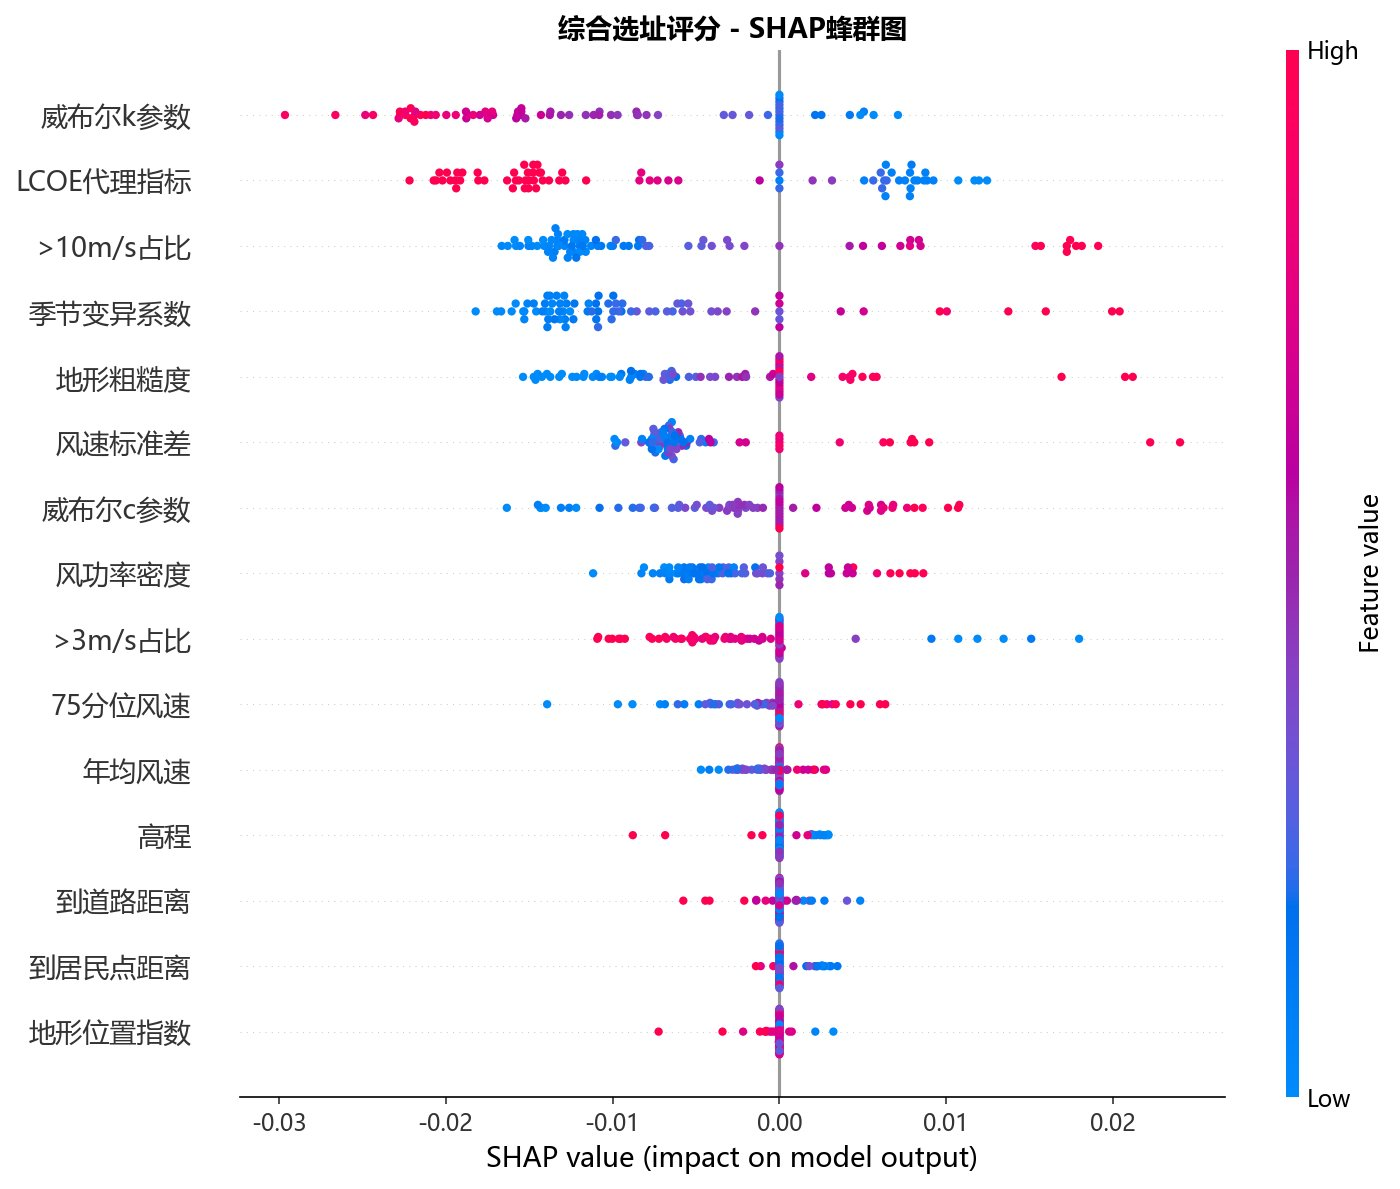
\includegraphics[width=0.85\textwidth]{shap_rank_beeswarm.png}
\caption{综合选址评分的SHAP蜂群图}
\label{fig:shap_beeswarm}
\end{figure}

\textbf{三个任务头的特征重要性差异。}
图~\ref{fig:shap_three_tasks}展示三个任务头的SHAP特征重要性对比，
揭示三个任务头学到了本质不同的选址决策逻辑。风资源评分头由风速
标准差、高于10\,m/s发电小时数占比和季节变异系数主导，三者共同刻画
风速的时间分布形态，与纯气候学风能评估框架一致。工程及政策合规头
则由LCOE代理指标独占主导地位，约占总SHAP权重的60\%，该任务头实质上
学到了距电网越近、地形越平坦则工程合规得分越高的决策规则。综合选址
评分头介于两者之间，威布尔$k$参数和LCOE代理指标并列主导，体现了
资源禀赋与工程约束的权衡。三个任务头特征重要性格局的显著差异表明，
GradNorm多任务架构并未发生任务坍塌，各任务头确实学到了互补的选址
决策依据。

\begin{figure}[H]
\centering
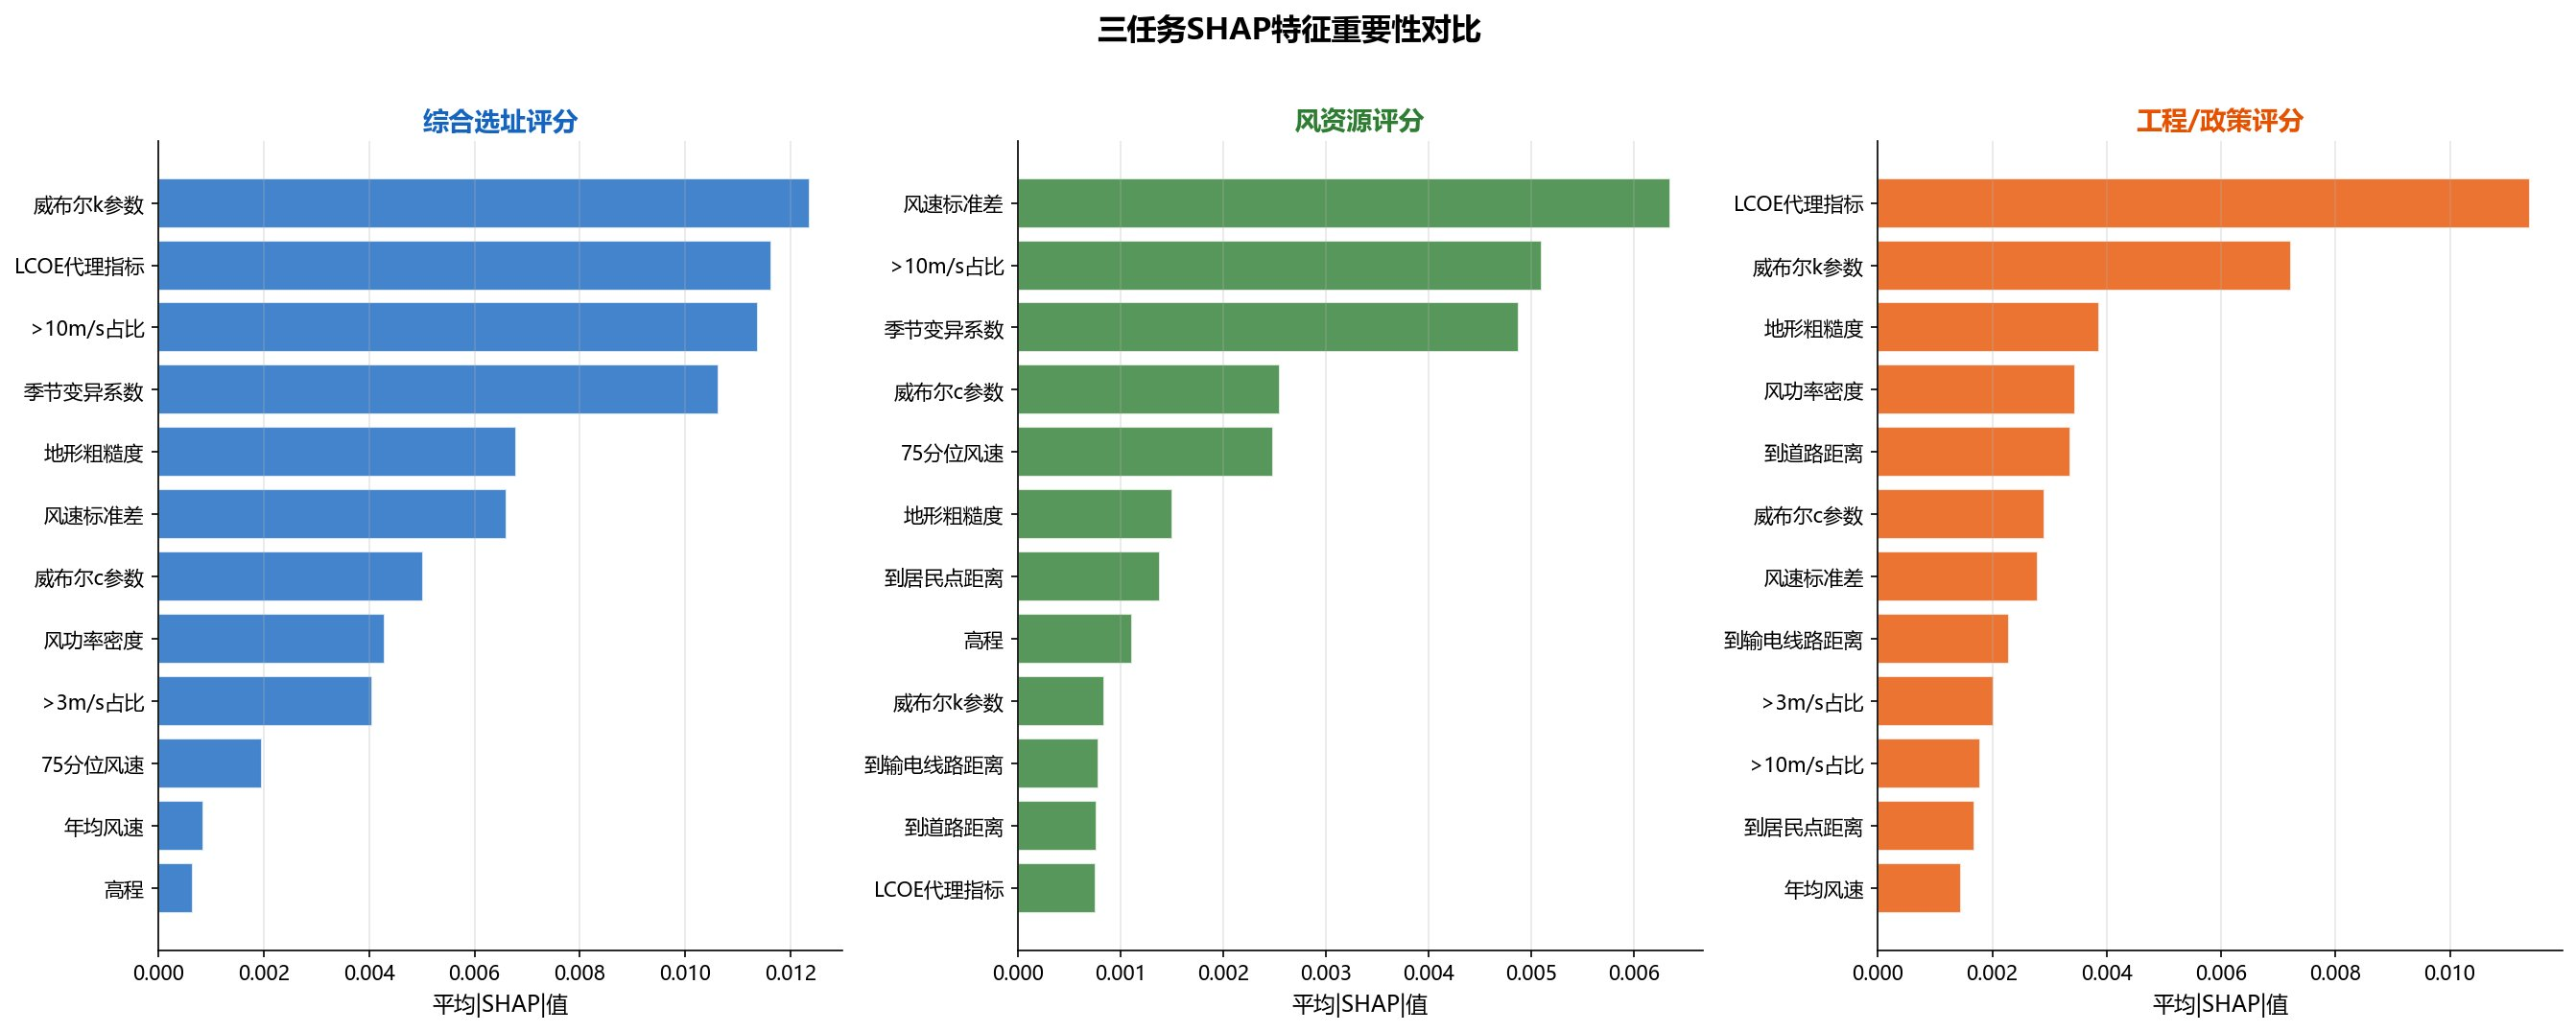
\includegraphics[width=0.98\textwidth]{shap_three_tasks.png}
\caption{三任务头SHAP特征重要性对比}
\label{fig:shap_three_tasks}
\end{figure}

\textbf{跨尺度特征重要性偏移。}
图~\ref{fig:shap_dumbbell}通过空心圆（实验一，SCADA，206个样本）与
实心圆（实验四OSM数据，9897个样本）的对比，揭示了从场址尺度到全国
尺度时特征重要性的系统性迁移，箭头方向表示从实验一到实验四的重要性
变化。最显著的偏移发生在到输电线路距离：该特征在实验一中重要性接近
零，而在实验四中跃升至全国尺度的主导地位。其背后的物理机制较为直接：
实验一的9个验证场址均为已建成并网项目，其选址本身已隐含电网可达的
前提条件，因此电网距离在该子集内变异极小；而实验四覆盖全国范围的
13197个格点，西部偏远格点与东部电网密集区之间存在数百千米的输电
距离差异，这一全国尺度的电网接入异质性被模型充分激活。相比之下，
威布尔$k$参数在两个实验中均保持高度稳定的重要性排名，表现出最强的
尺度不变性，验证了将其纳入特征集的必要性~\cite{jung2021}。政策流
特征在两个实验中均贡献约31\%的SHAP总量，与消融实验的结论相互印证。

\begin{figure}[H]
\centering
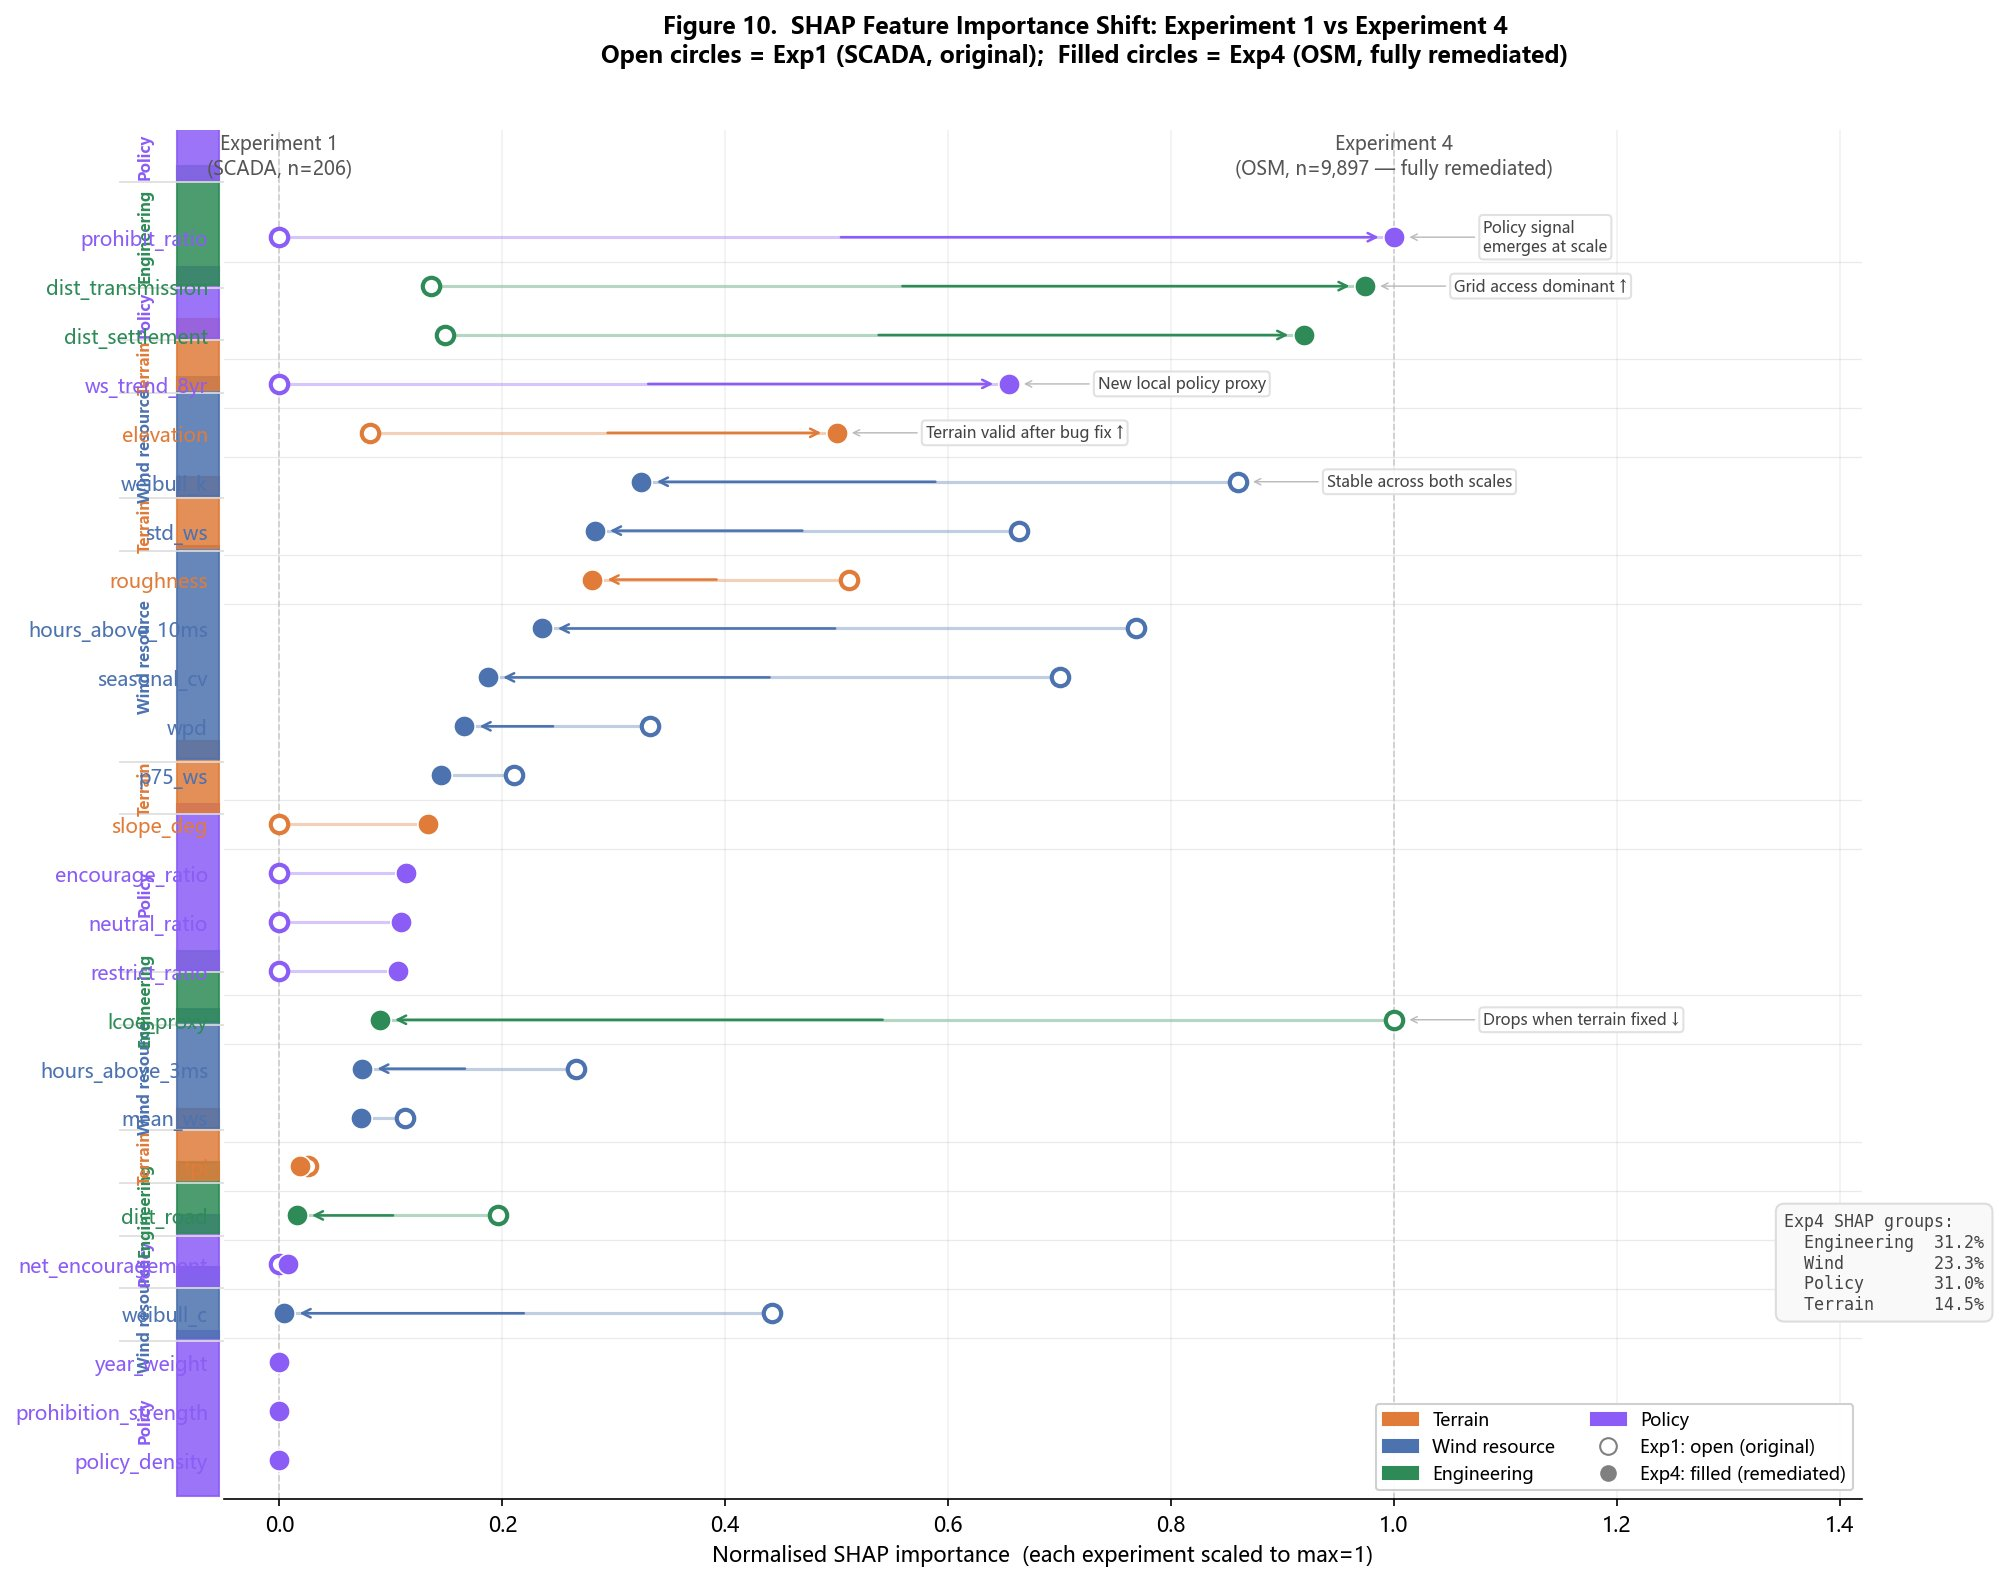
\includegraphics[width=0.95\textwidth]{figure10_dumbbell_v4.png}
\caption{SHAP特征重要性跨尺度偏移}
\label{fig:shap_dumbbell}
\end{figure}

\subsection{独立验证场址空间分析}

图~\ref{fig:corr_heatmaps}展示九个独立验证场址基于2019至2020年ERA5
100\,m风速计算的Pearson相关系数热力图，每图覆盖以推断场址位置为中心
的$\pm5^\circ$空间窗口。Sites\,1、2、6和7的推断位置均位于局部相关系数
高值区，坐标置信度较高；喀什场址呈现近似均匀的低相关平坦分布，证实
坐标推断不可靠，已排除。

\begin{figure}[H]
\centering
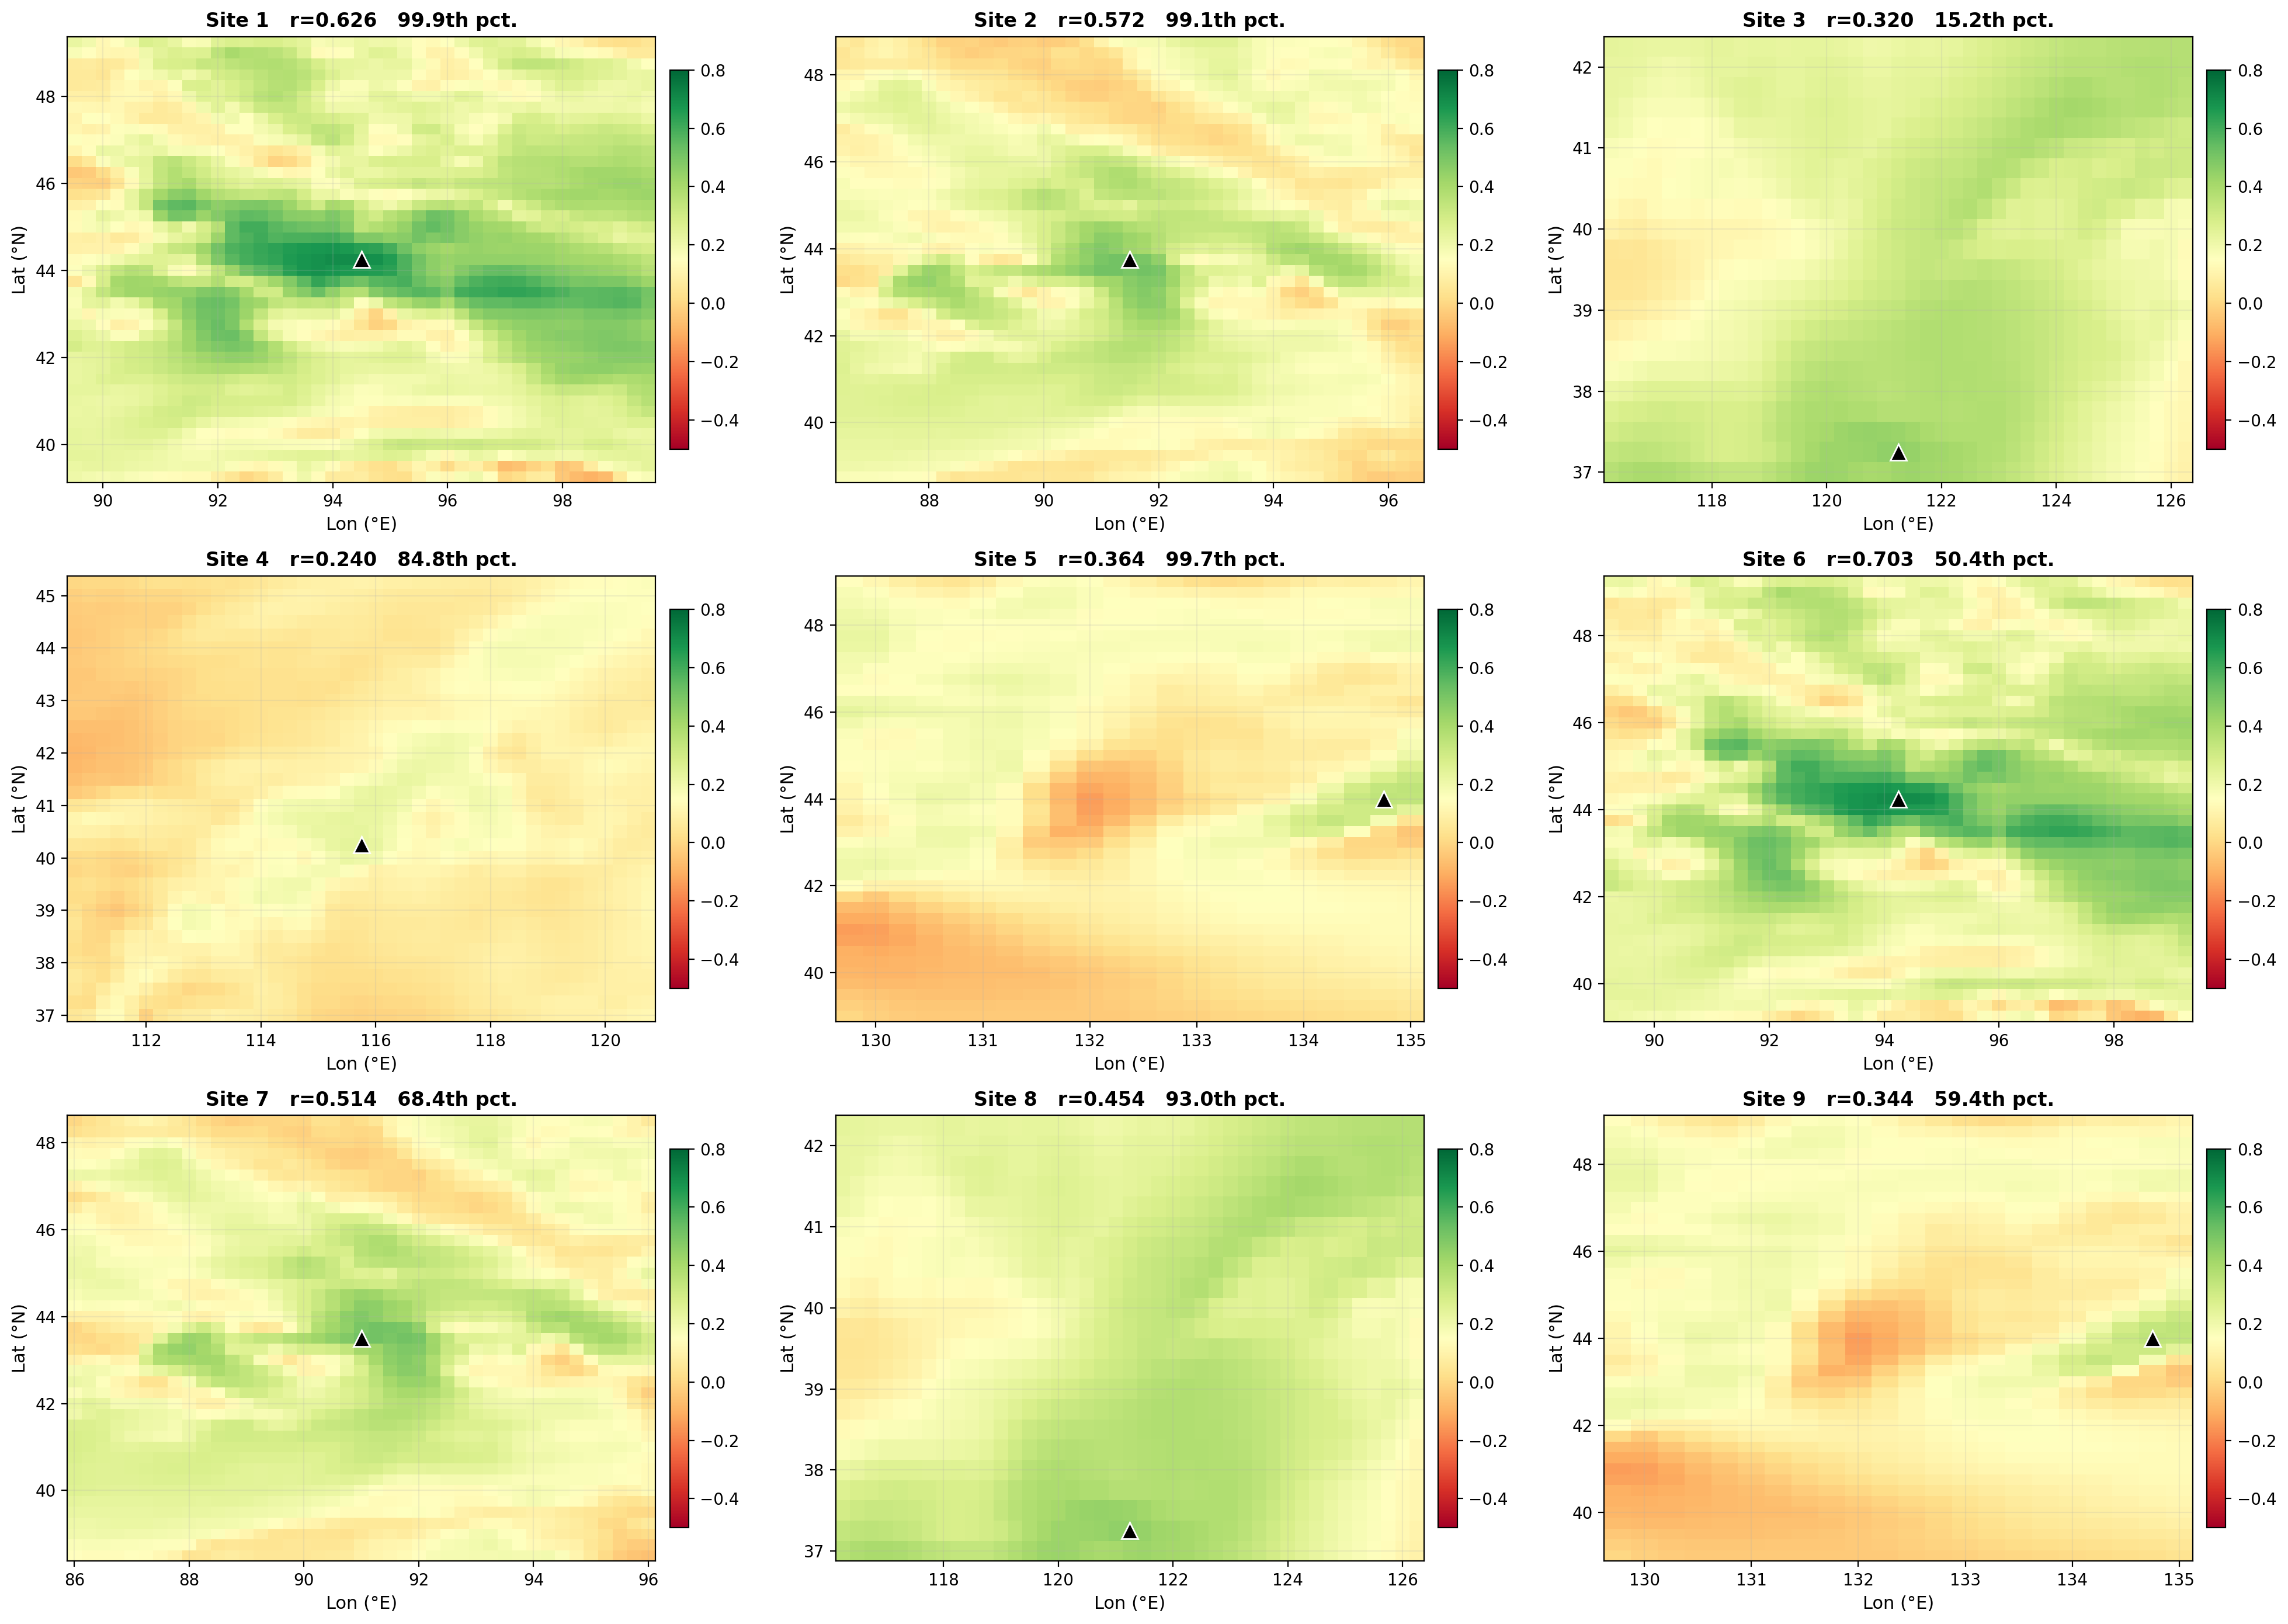
\includegraphics[width=0.95\textwidth]{C_correlation_heatmaps.png}
\caption{九个独立验证场址ERA5相关性热力图}
\label{fig:corr_heatmaps}
\end{figure}

图~\ref{fig:sensitivity}进一步检验坐标推断可靠性：面板A显示在阈值
0.0至0.3范围内AUC稳定在0.79至0.82，模型性能对低置信度场址不敏感；
面板B显示在55\,km以内位移误差下AUC始终在基线5\%误差带以内，坐标
推断误差在合理范围内不影响评估可靠性。

\begin{figure}[H]
\centering
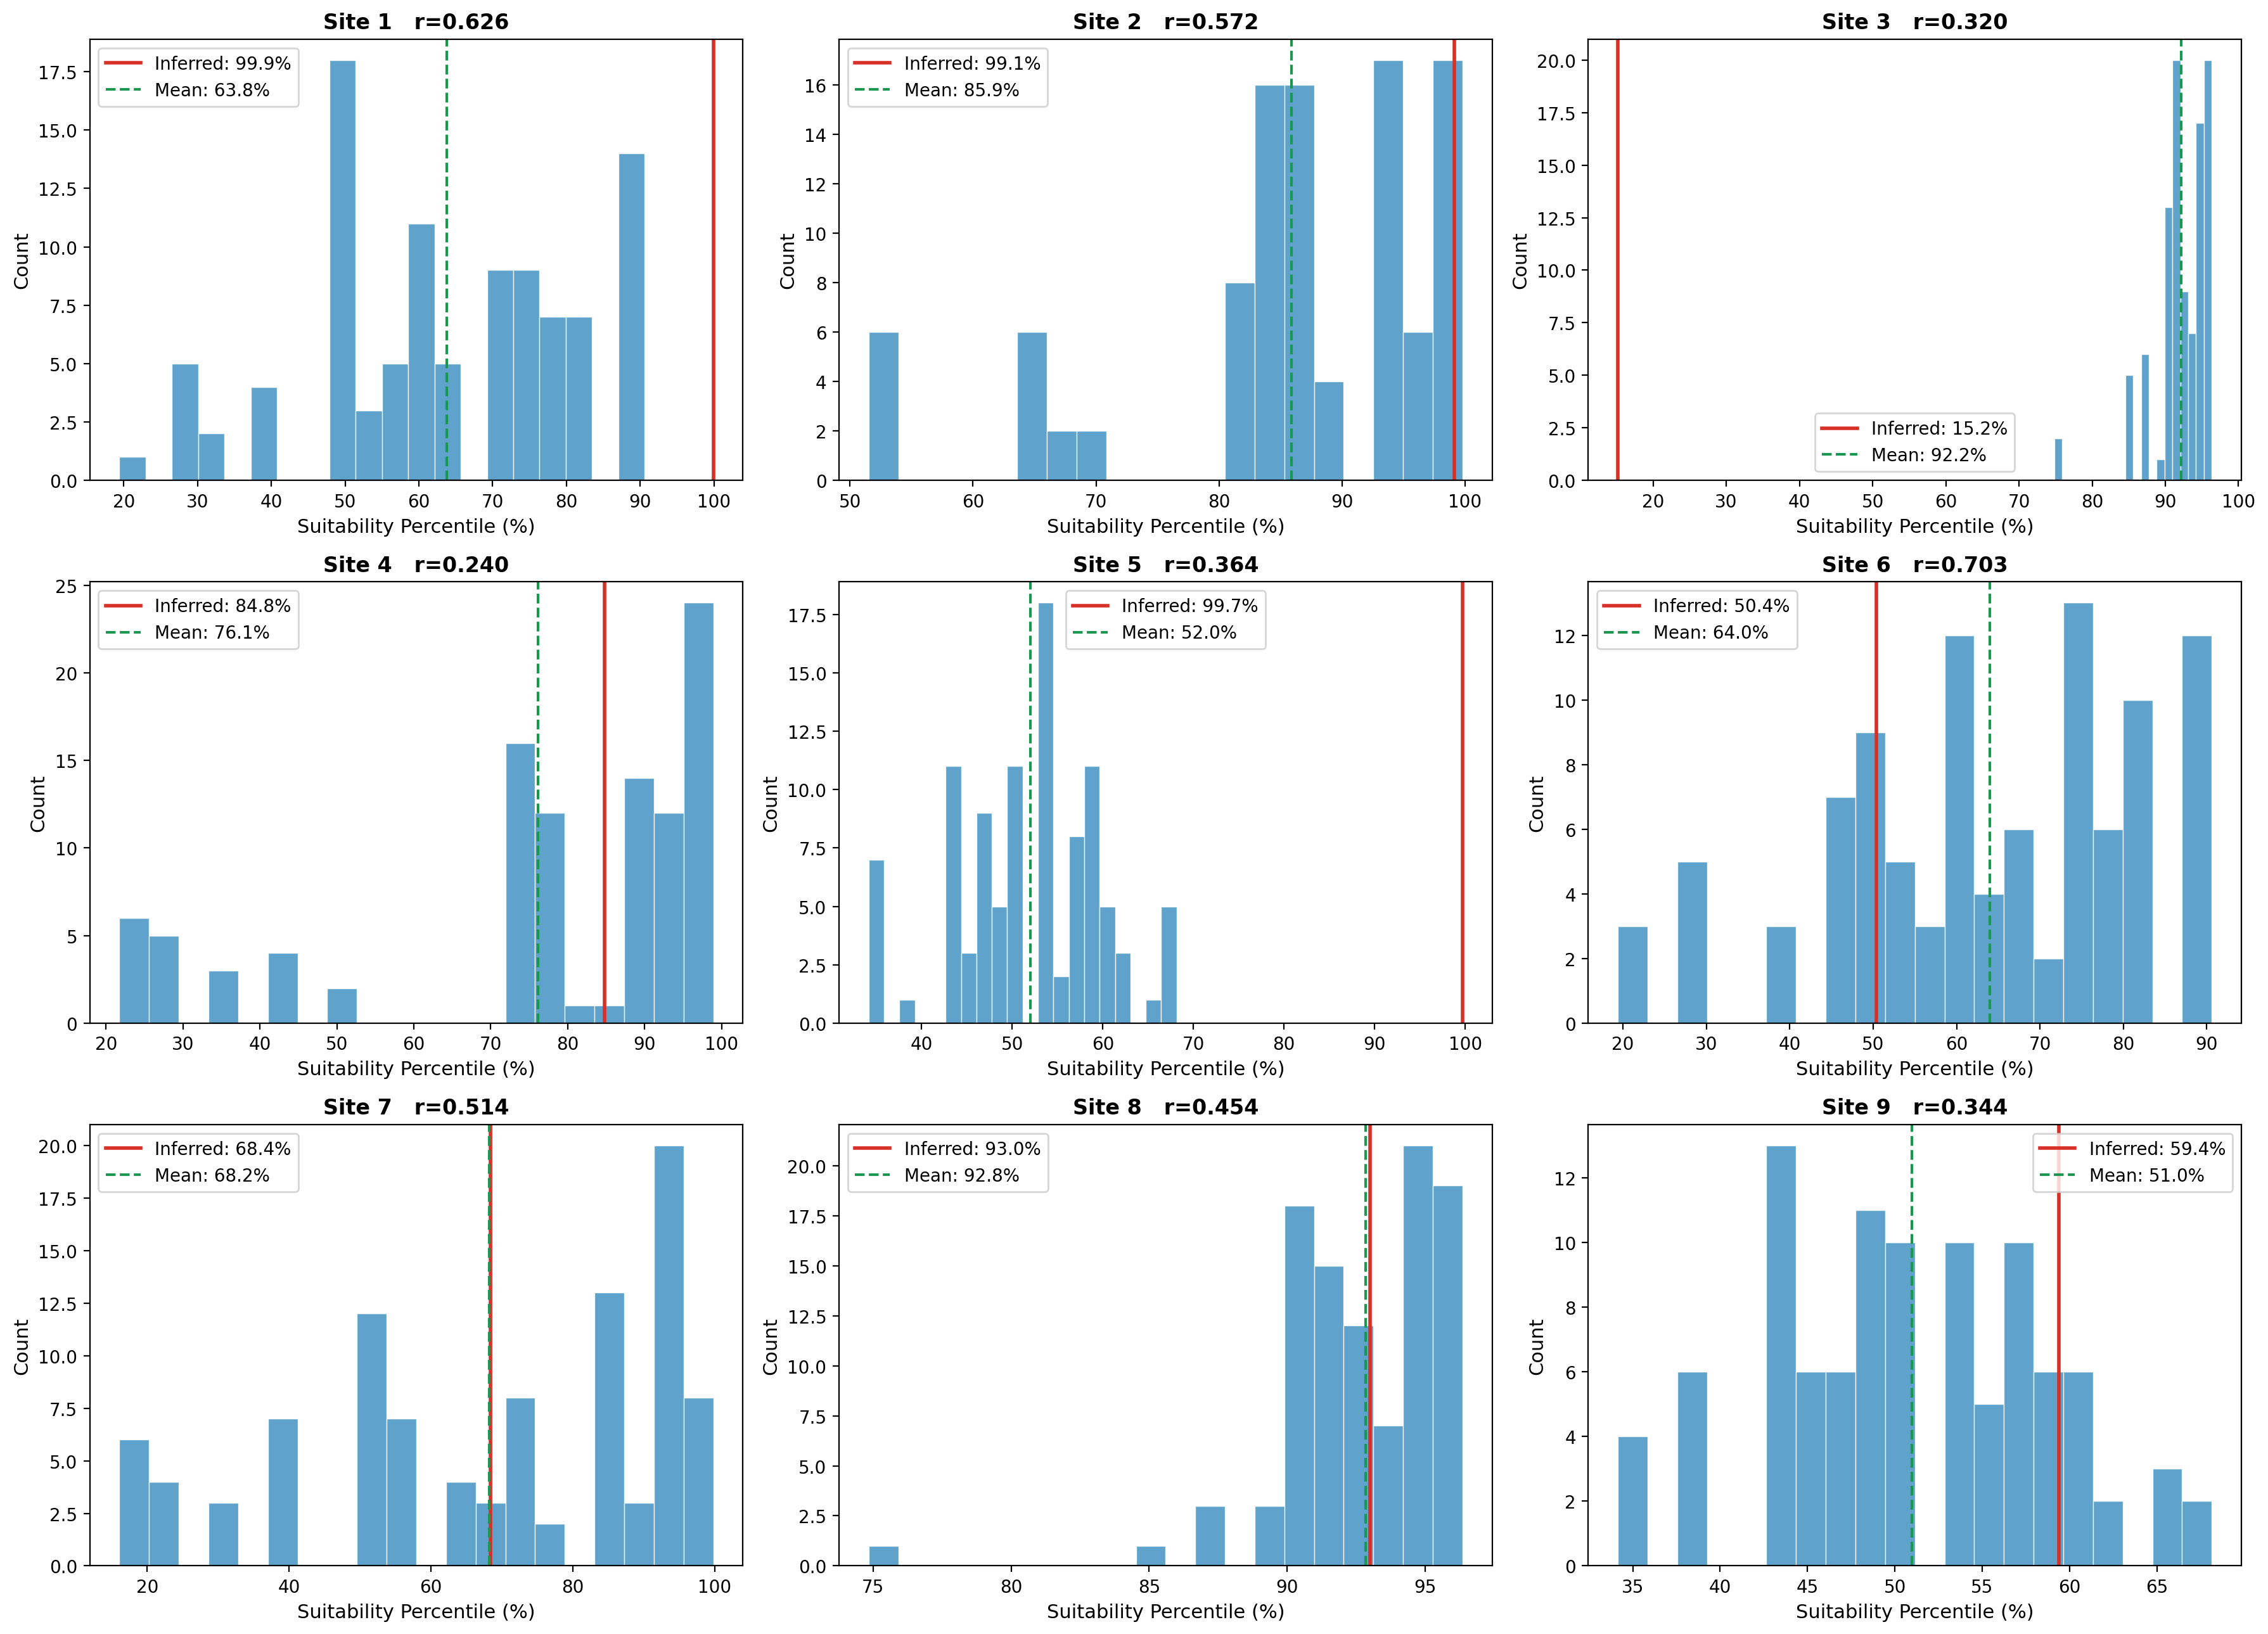
\includegraphics[width=0.92\textwidth]{sensitivity_summary.png}
\caption{坐标推断可靠性敏感性分析}
\label{fig:sensitivity}
\end{figure}

在全部13197个格点上按场址排名得分排序，Sites\,1、2和5分别排入全域
第10、115和40位，全部进入前200；Site\,8排名第923位；Top-3000内共
召回5个场址（召回率0.556）；Top-7000内召回8个场址（召回率0.889）。
AUC=0.8970表明模型对完全未参与训练的真实运行场址具有较强泛化能力，
Sites\,1和2（新疆，$r\geq0.57$）被分配至极高适宜区核心，与风资源
禀赋和电网条件高度吻合。

为进一步量化验证结论的稳健性，对九个独立验证场址实施留一法交叉验证，
并与随机基线和仅风速排序基线进行对比，结果如图~\ref{fig:scada_loo}
所示。面板a为各场址留一法百分位；面板b为五维雷达图（适宜性百分位、
年均风速、风速稳定性、ERA5相关系数、电网可达性）；面板c为
Top-$K$召回率曲线。

留一法结果显示：Sites\,1、2、5均排入前200（百分位分别为99.9\%、
99.1\%、99.7\%）；Site\,4（张家口，84.8\%）排入前3000；Site\,3
（山东，15.2\%）排名偏低，与东西向泛化局限一致，山东属于108$^\circ$E
以东的季风气候区。高置信度场址在适宜性百分位和风速稳定性维度均明显
优于低置信度场址，支持循环性对结果影响有限的论断。

Top-$K$召回率曲线显示，本文模型在Top-500时召回率0.333，是随机期望值
（0.038）的8.8倍（二项检验$p<0.01$）；Top-3000时召回率0.556，
Top-7000时达0.889。仅风速排序基线在Top-500时召回率为零，Top-1000时
仅0.111，显著低于本文模型，证明多特征融合框架相比单一气候指标具有
实质性判别优势。九个场址平均适宜性百分位74.4\%，Bootstrap 95\%置信
区间为54.9\%至90.9\%，中位数84.8\%。

\begin{figure}[H]
\centering
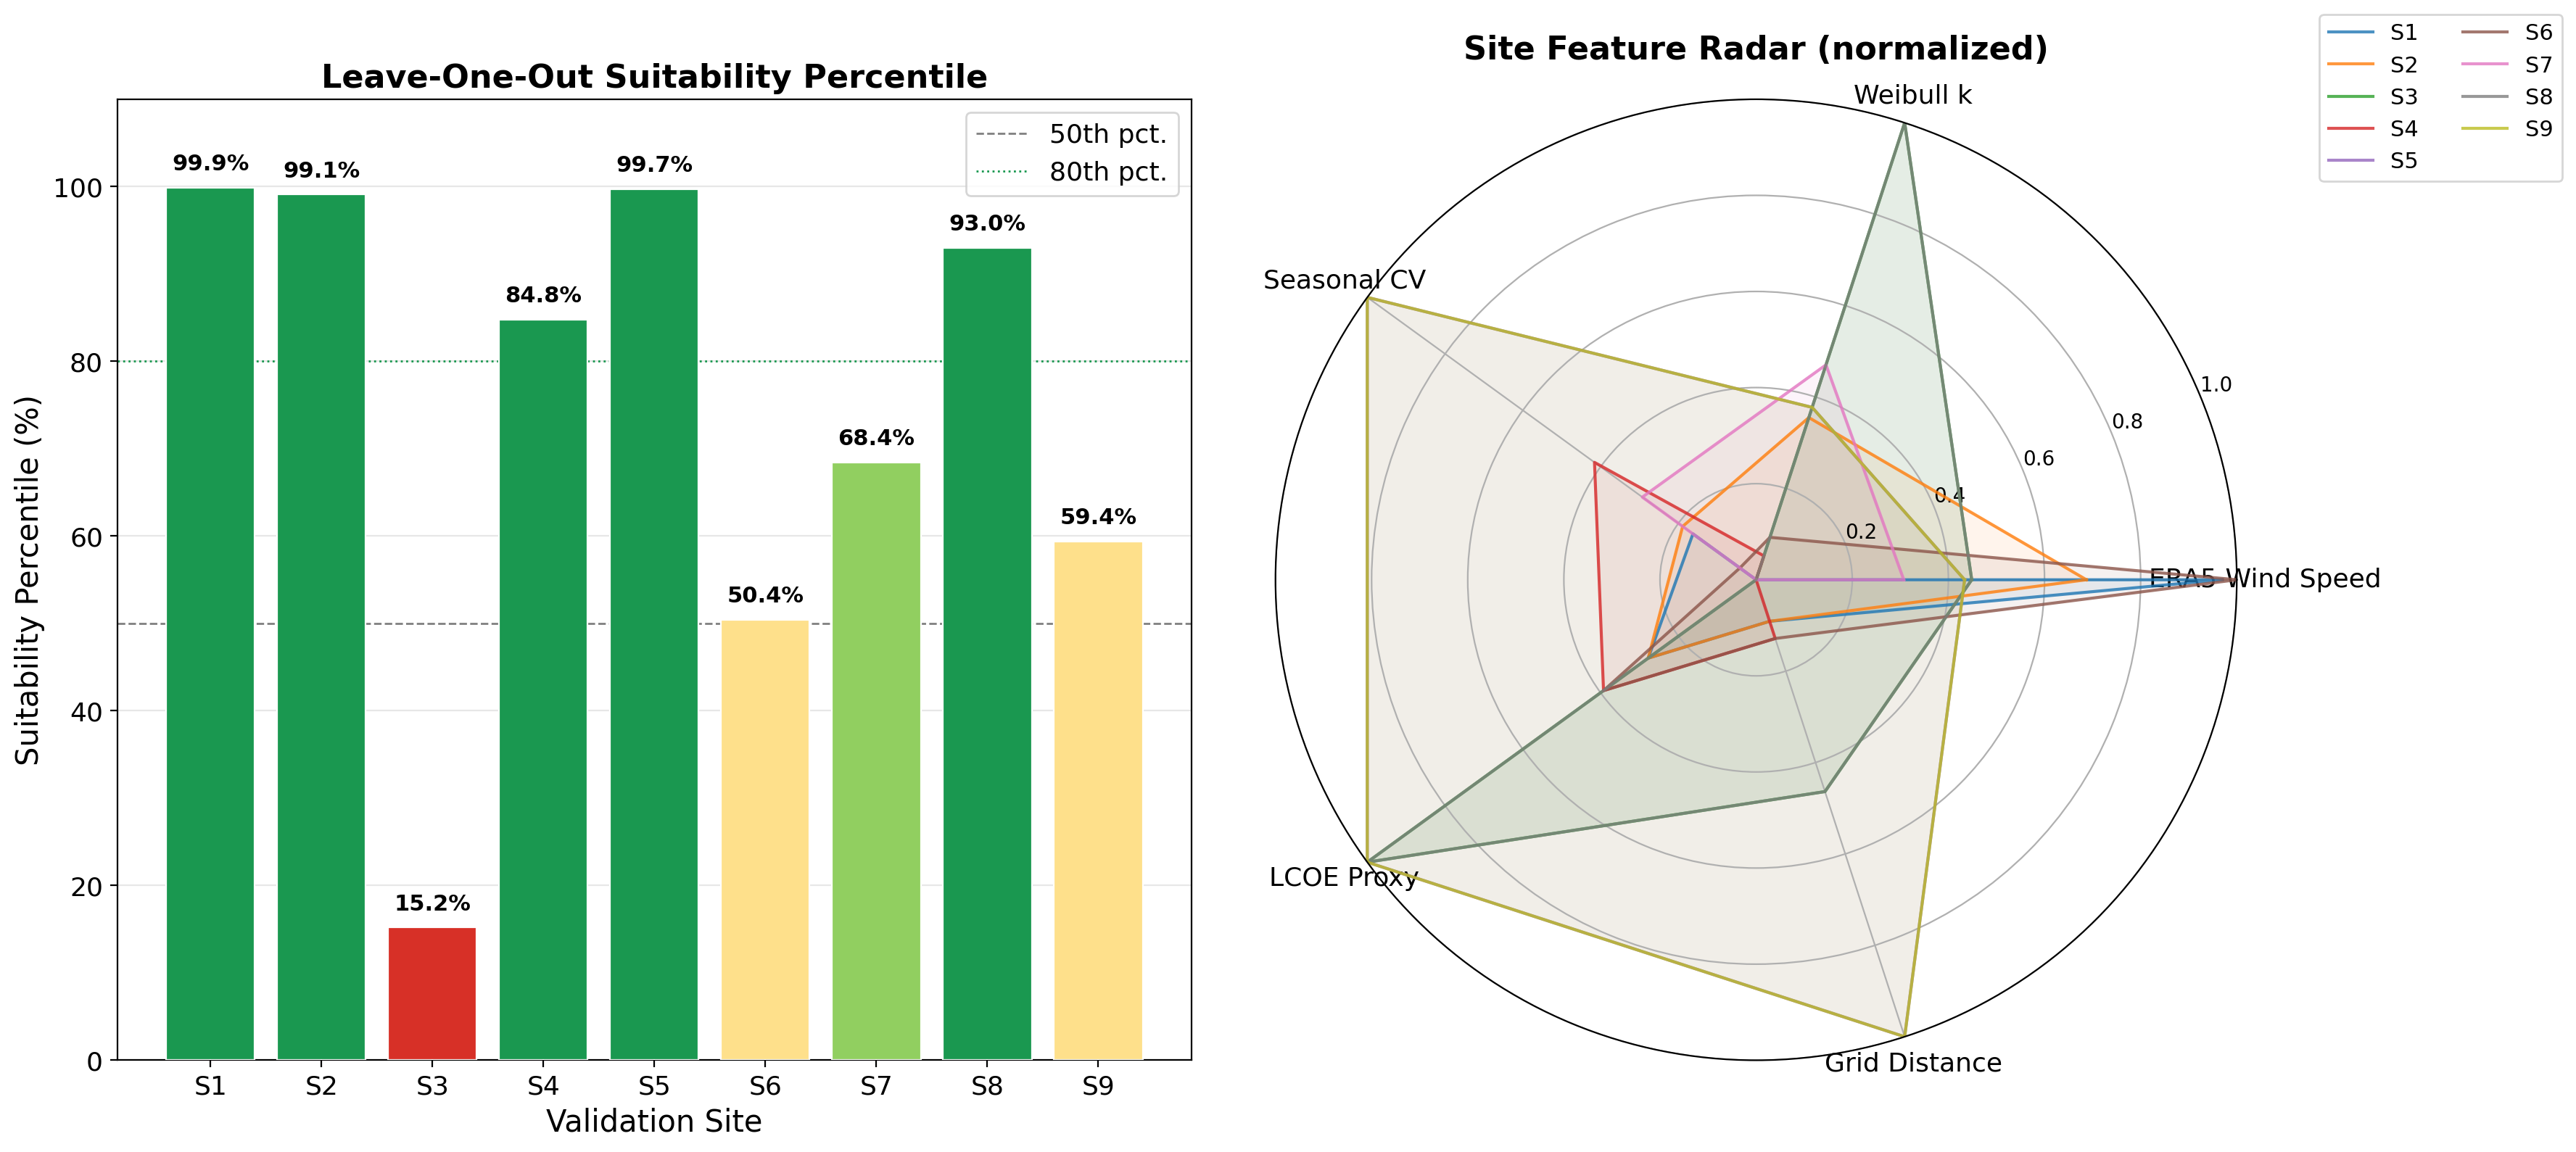
\includegraphics[width=0.98\textwidth]{scada_loo_radar.png}
\caption{独立验证场址留一法分析}
\label{fig:scada_loo}
\end{figure}

\subsection{风电场适宜性地图}

图~\ref{fig:suitability}展示全国13197个格点的场址排名适宜性地图，
颜色按五分位阈值划分为极高（深红，前20\%）、高（橙色，60至80\%）、
中等（黄色，40至60\%）、低（浅蓝，20至40\%）和极低（蓝色，后20\%）
五类适宜等级；九个独立验证风电场以三角形标注，相关系数不低于0.5者
用实心星形，0.3至0.5者用空心三角形，低于0.3者用倒三角形。

高适宜区排名分不低于第60百分位，总面积420521\,km$^2$，集中于以下
四个区域：新疆107355\,km$^2$，以哈密至吐鲁番走廊为核心；
内蒙古97397\,km$^2$，主要分布于锡林郭勒高原；甘肃53674\,km$^2$，
位于河西走廊；吉林37738\,km$^2$，覆盖松辽平原西部。Sites\,1、2、6和7位于新疆极高或高适宜区，Sites\,3和4分别位于
山东和张家口的中至高适宜区，Site\,5（黑龙江）位于东北高适宜区，
Sites\,8和9与Sites\,3、5推断位置相近，百分位结果一致。

上述高适宜区的空间格局具有较强的地理可解释性。新疆和内蒙古因稳定
的西北气流和平坦地形呈现最高的威布尔$k$值，SHAP分析已证实这是综合
选址评分的第一主导特征；甘肃河西走廊兼具高风速与现有输电基础设施
密集的双重优势，使LCOE代理指标同样处于有利区间；东北吉林则得益于
松辽平原坡度极小（均值低于0.5$^\circ$）且省级政策持续鼓励的综合
效应。这一结果与《"十四五"可再生能源发展规划》~\cite{ndrc2022}和
《"十五五"规划纲要》~\cite{ndrc2026}划定的风电优先开发区域高度
吻合~\cite{he2023,zhong2022}，表明模型输出具备较强的政策一致性。

\begin{figure}[H]
\centering
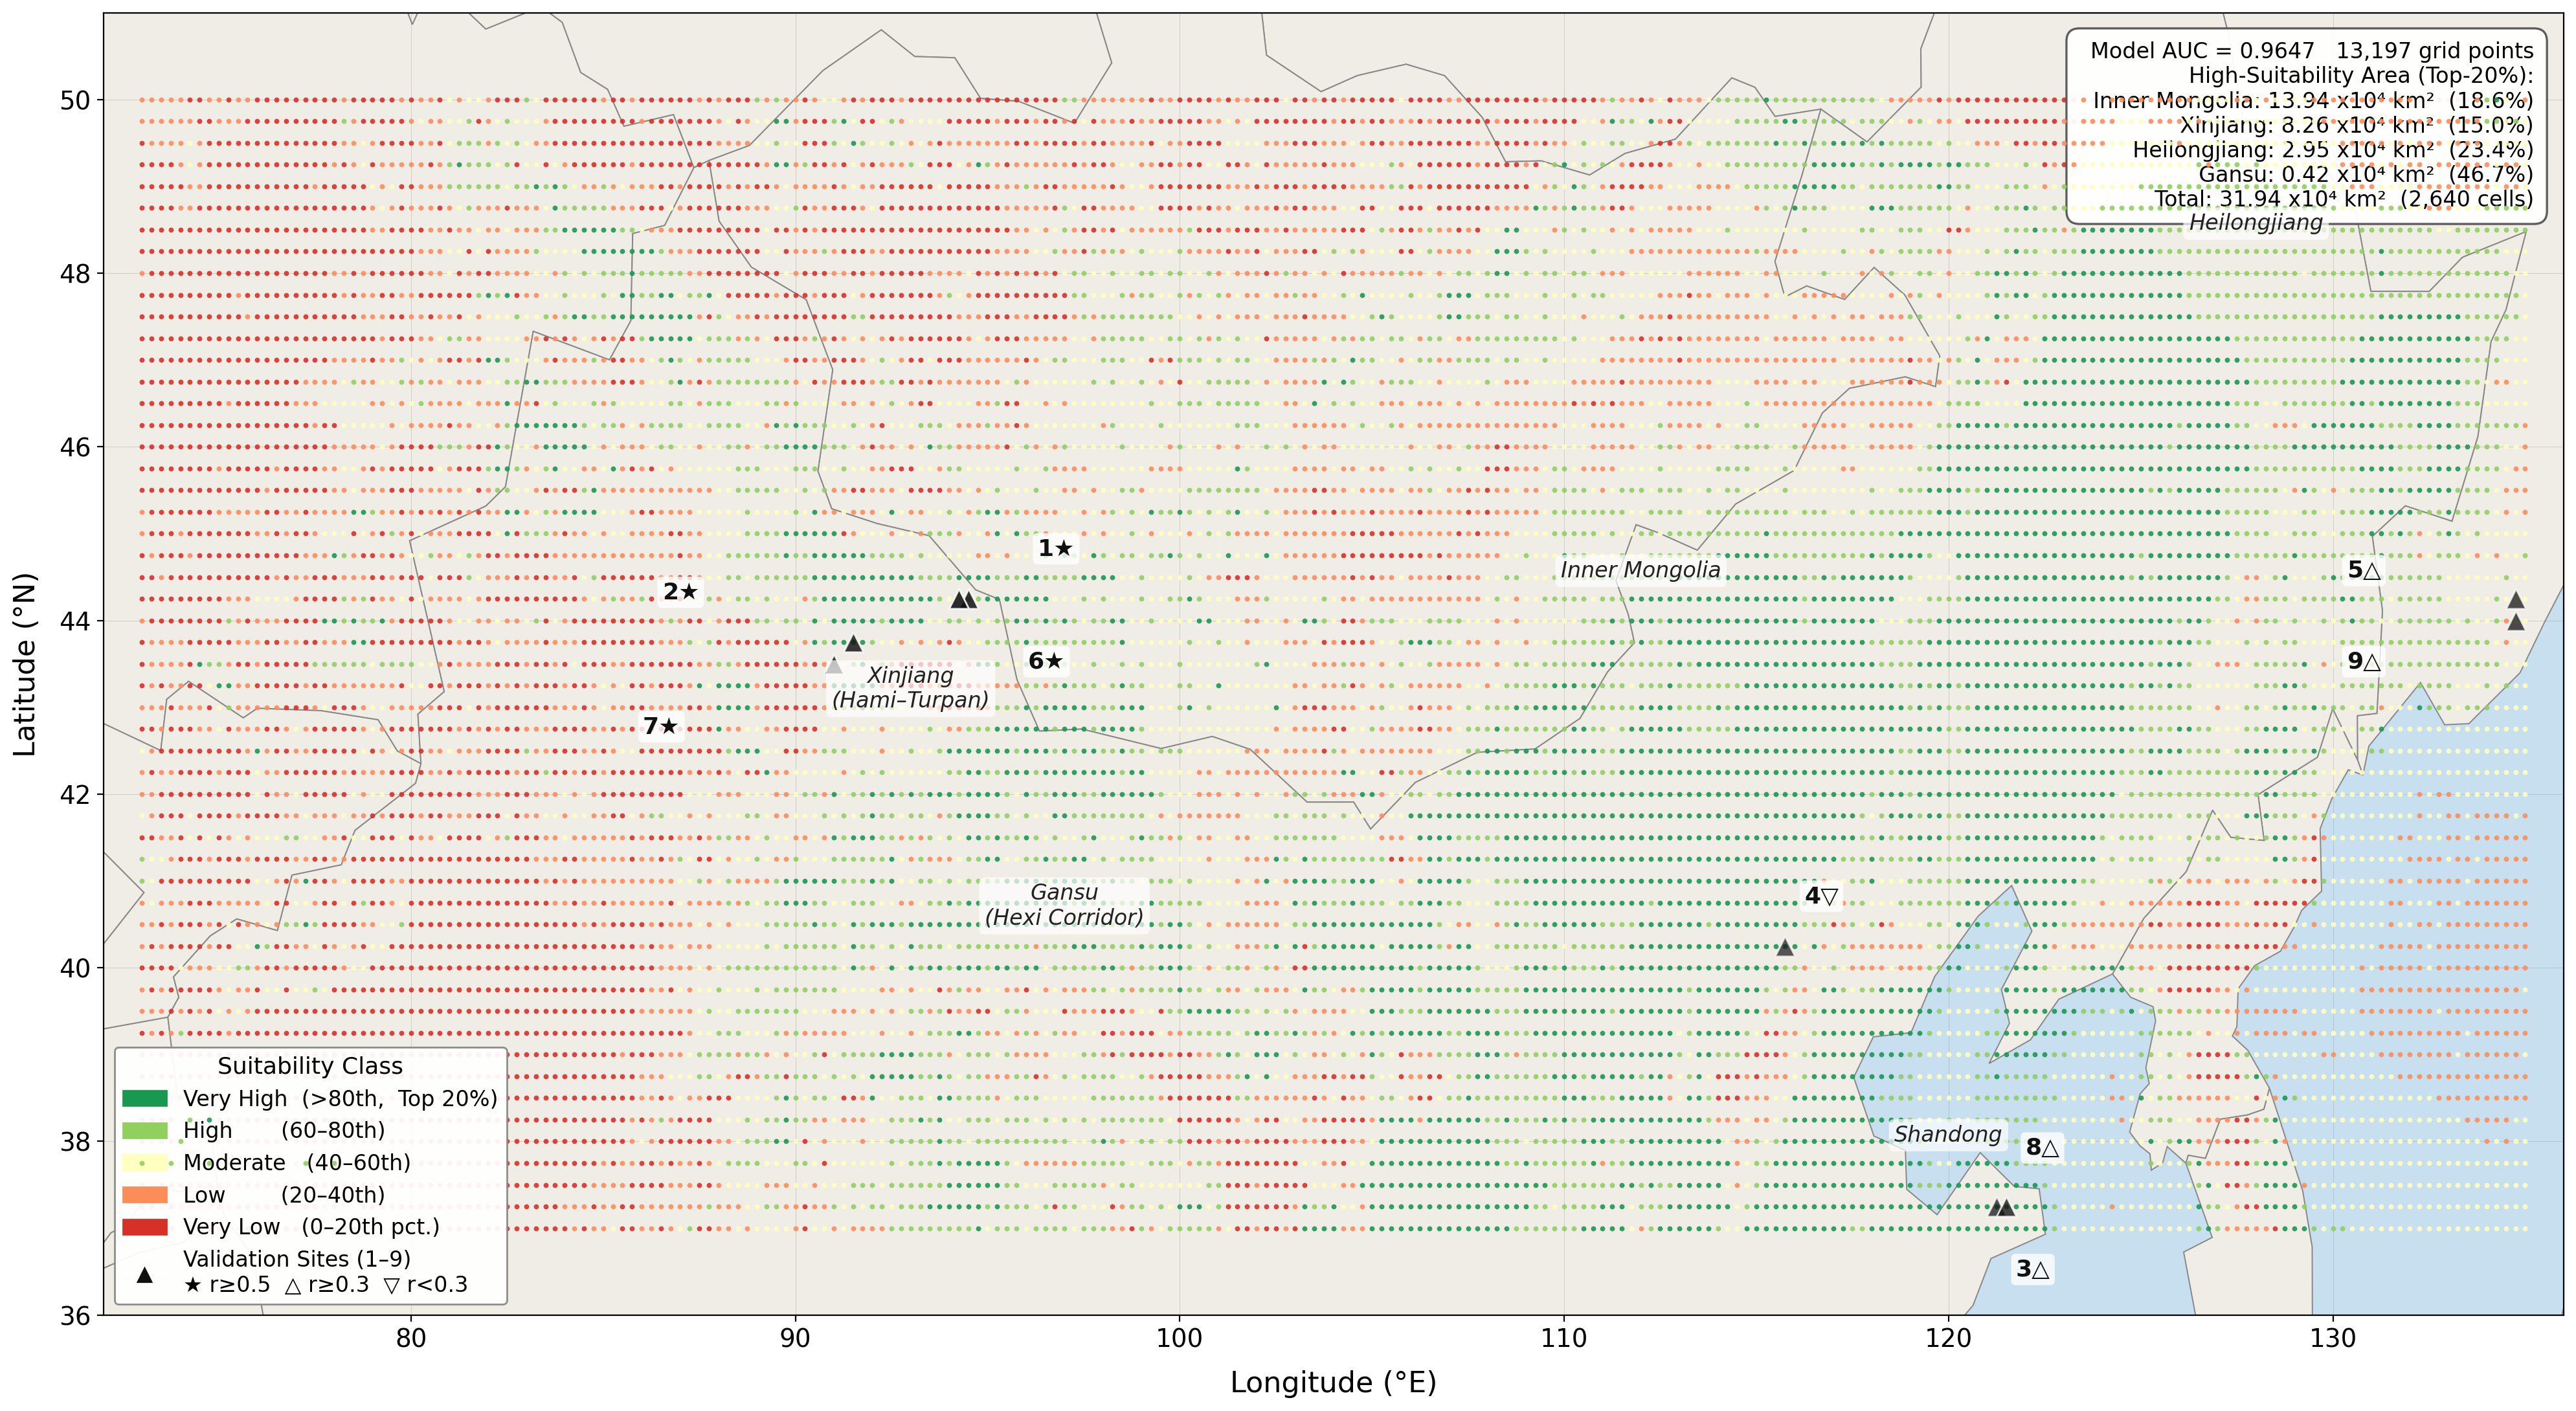
\includegraphics[width=0.98\textwidth]{suitability_map_final_v2.png}
\caption{风电场选址适宜性地图}
\label{fig:suitability}
\end{figure}

% ============================================================
\section{讨论}
% ============================================================

本节围绕三个核心议题展开讨论：本框架相对现有方法的优势来源、
实验二揭示的地理泛化局限及其背后机制，以及消融实验与SHAP分析之间
的表面矛盾与统一解释。最后归纳框架的适用边界与主要局限。

\subsection{与现有研究的对比}

Bilgili等~\cite{bilgili2024}在土耳其数据集上以XGBoost实现96.07\%准确率，
将政策约束处理为预处理阶段的二值掩码。本框架在更大规模中国数据集上，
引入BERT+LoRA政策语义流后$\Delta\text{AUC}=+0.0820$，且在省级分层基准
AUC=0.9950的水平上仍统计显著优于XGBoost（$p=0.019$），证明将政策语义
纳入端到端训练具有实质性优势。

Chen等~\cite{chen2026}同样将政策合规性作为后处理掩码。本框架的改进在于
句子级BERT嵌入保留了四类监管意图的语义梯度，SHAP分析提供跨三个任务头
的可解释性，九个独立验证场址提供外部效度证据。

表~\ref{tab:ablation_policy}已排除"政策流等价于省份标签"的竞争性解释：
控制省份信息后BERT+LoRA仍贡献$\Delta\text{AUC}=+0.0790$（$p=0.002$），
AHP与TOPSIS在同测试集上AUC分别仅为0.6960和0.6910，与本框架相差约30个
百分点，表明传统多准则决策分析方法在高维非线性选址问题上存在根本局限。

\subsection{地理泛化局限}

实验二（AUC=0.6710）揭示模型在跨越108$^\circ$E气候分界时的泛化局限。
108$^\circ$E以西正样本仅占总量20.9\%，KS检验证实东西两侧正样本在
威布尔$k$参数（KS=0.638，$p<0.001$）、季节变异系数（KS=0.486）、
年均风速（KS=0.202）上均存在显著分布差异，导致分布外泛化失败。
该边界与胡焕庸线~\cite{chen2016huline}高度吻合——这一经典地理
分界线将中国干旱西北与湿润季风东南分隔开来~\cite{zhao2023windchina}，
证明模型性能下降反映的是真实气候不连续性而非模型缺陷。
引入东部沿海正样本和领域自适应技术是主要改进方向。

\subsection{政策流与SHAP的统一解释}

消融实验显示去除政策流后AUC下降0.1050（$p=0.002$），而SHAP政策特征
重要性均不超过0.03。两者不矛盾：消融反映政策流作为省级正则化项对全局
模型的影响，SHAP测量格点级边际贡献——同省格点共享相同政策向量，格点级
贡献趋近于零是省级分辨率的固有属性。门控值空间分布（图~\ref{fig:gating_map}）
印证了这一机制：108$^\circ$E以西$g$值整体偏高，政策流在省际尺度产生
了差异化的软约束效果，$g$值全域低于0.5，数值流始终保持主导地位。

\subsection{门控值$g$的地理机制与跨模态注意力验证}
\label{sec:gating}

Sigmoid门控值$g$提供了一个独特的可解释性窗口，揭示政策语义在何处
以何种方式影响选址决策，并为跨模态注意力机制在学习有意义的地理结构
而非充当黑盒这一论断提供了直接证据。

图~\ref{fig:gating_map}展示全部13197个格点的$g$值空间分布及省级
箱线图，呈现出三个显著的地理规律。

第一，新疆和甘肃$g$值系统性偏高（中位数0.33至0.35），108$^\circ$E以东
出现明显低$g$带。这一东西向对比有文献数据的实证支撑：本文第3.4节
政策语料库显示，宁夏（5.0\%）、内蒙古（4.7\%）和甘肃（4.1\%）的鼓励
类条款比例远高于吉林（1.4\%）和新疆（0.6\%，新疆省级文件以框架性语言
为主而非场址使能型承诺）。模型捕获了这一逻辑：新疆风资源全球一流，
但省级政策对具体场址的赋能程度远低于甘肃和宁夏，$g$值上升正是编码了
资源禀赋与政策推动力之间的这种张力。东部格点输电基础设施密集，开发
决策主要由局地地形和风速决定，$g$值相应下降，数值流主导。

第二，门控四分位距最宽的两个省份——山东和宁夏——恰好是政策内部
异质性最高的省份。山东将沿海离岸风电激励与内陆生态保护缓冲区并置；
宁夏同时鼓励戈壁大型装机并保护灌溉农业用地。这一IQR规律包含重要的
理论含义：尽管同省格点共享相同的政策嵌入向量$\mathbf{F}_\text{policy}$，
模型依然根据各格点自身的数值属性——LCOE代理指标、威布尔$k$值、
输电线路距离——动态调整$g$值，选择性地吸收政策语义。这正是
\textbf{数值引导的语义检索}：跨模态注意力执行的不是省份查表，而是
以局地物理属性为查询键、主动检索最相关政策语义的动态加权过程。

第三，尽管$g$值存在空间差异，但全域始终低于0.5，确认数值流保持全局
主导地位，政策流作为选择性放大器而非主导驱动力运作。省级中位$g$值
排名（辽宁0.36、陕西0.34、吉林0.32、河北0.27）进一步反映了各省开发
潜力受行政而非气象因素制约的程度，与历史投资记录总体吻合。

综上，$g$值的非均匀空间分布——具备可解释的东西向梯度、与政策密度
的对应关系、以及省内自适应方差——构成跨模态注意力模块已内化中国风电
治理空间逻辑的后验验证。若$g$值空间均匀，则说明门控机制未能习得任何
有意义的结构；我们观察到的异质性模式，正是该机制在执行\textbf{数值引导
语义检索}的直接证明。

\begin{figure}[H]
\centering
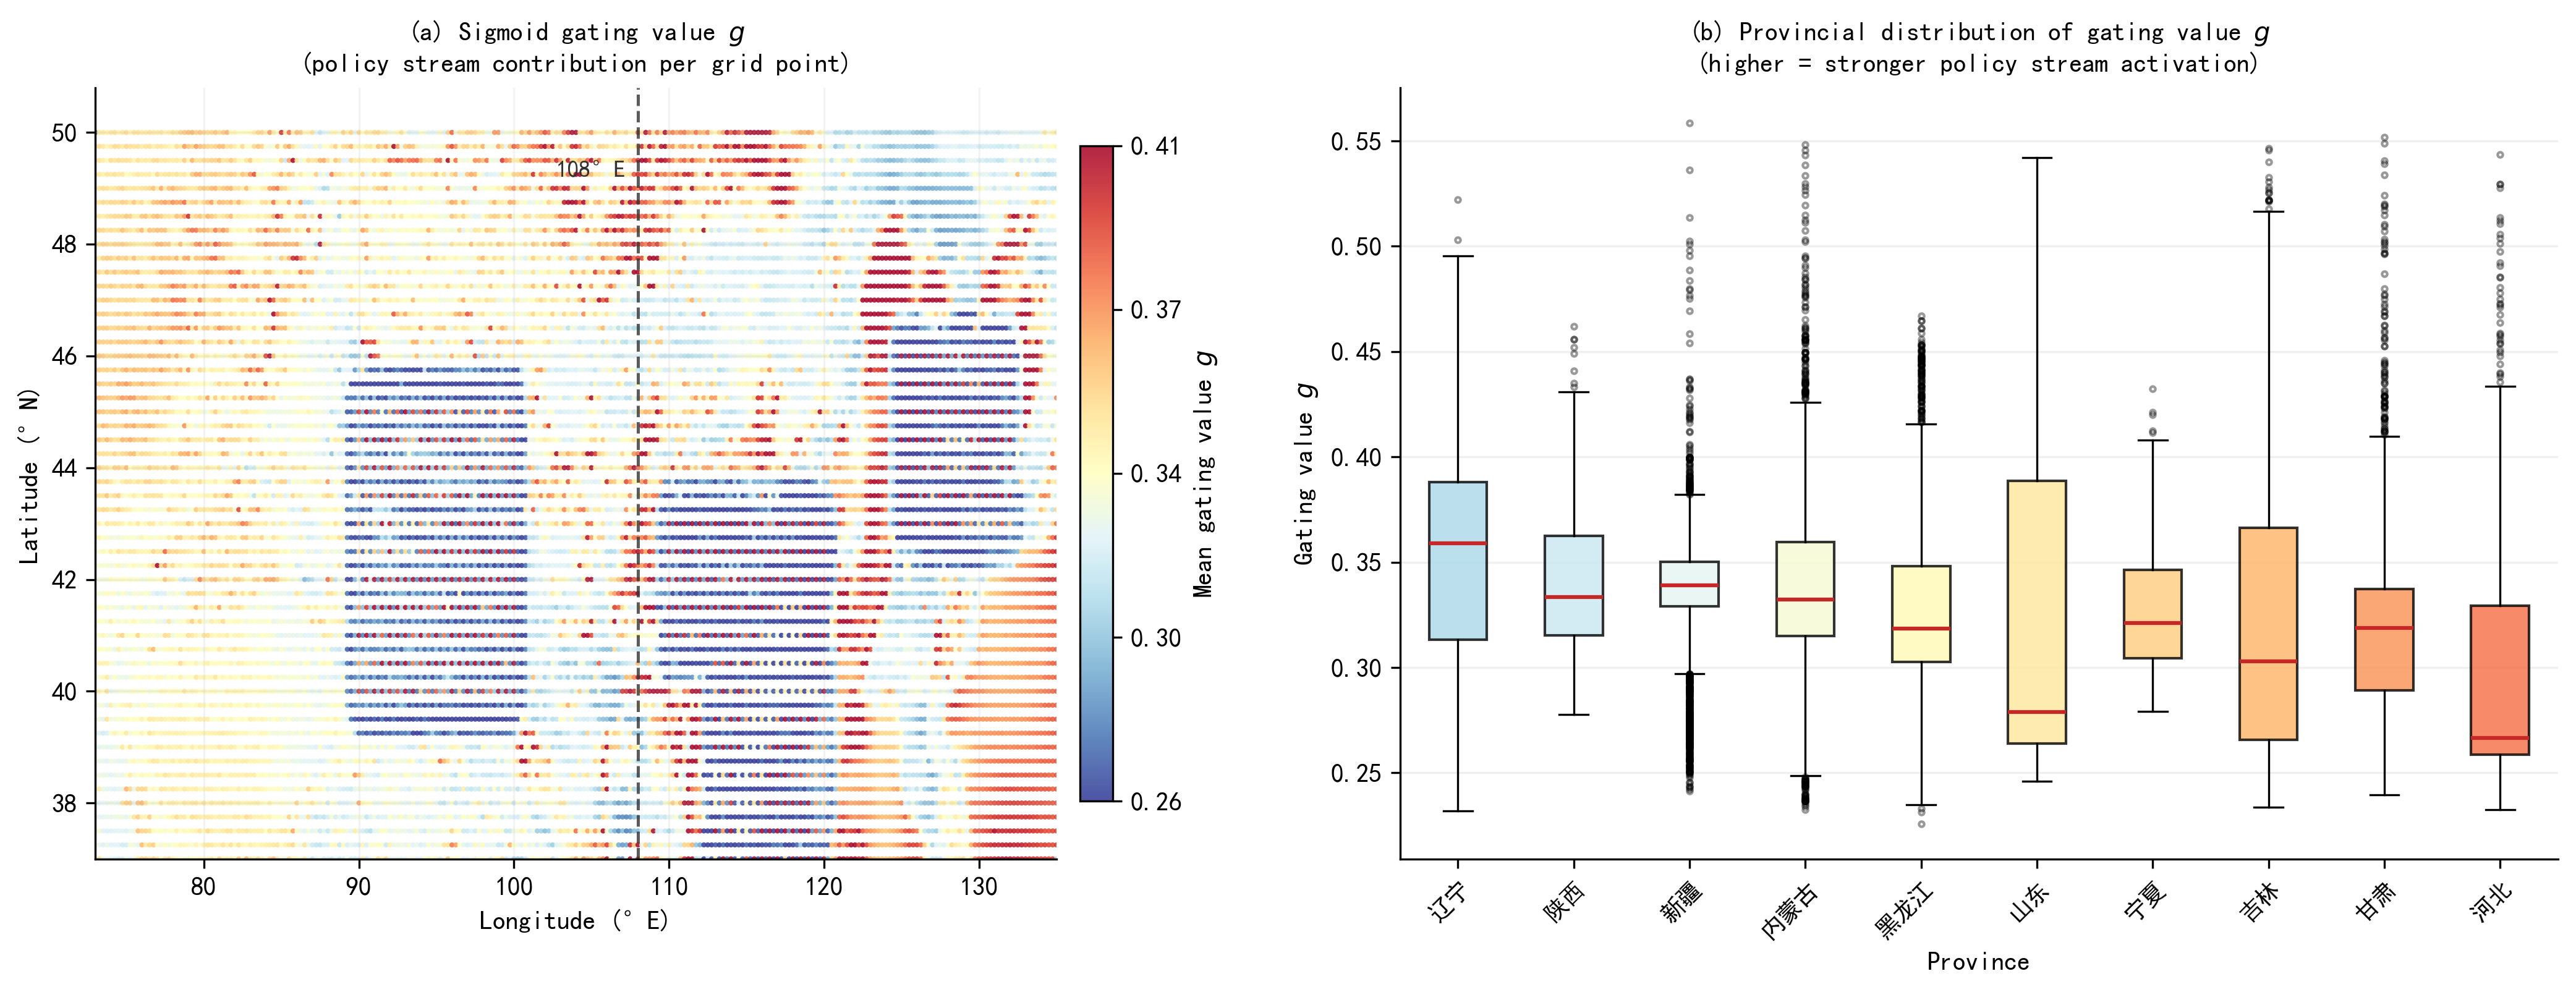
\includegraphics[width=\linewidth]{gating_map.png}
\caption{Sigmoid门控值空间分布与省级分布}
\label{fig:gating_map}
\end{figure}

\subsection{局限性与展望}

本框架当前的主要约束来自三个方面。验证坐标通过ERA5相关性推断，与模型
输入存在部分数据重叠；敏感性分析表明55\,km以内位移误差对AUC影响在5个
百分点以内，留一法验证结论稳健，但获取官方运营坐标仍是根本解决途径。
政策语料库覆盖六个重点省份14份省级文件，地市级法规尚未纳入，省级
嵌入分辨率受限于行政边界粒度；后续可随地市级法规数字化逐步扩充。
ERA5在复杂山地地形的系统性低估（0.3至1.5\,m/s）导致西藏、云贵高原
评分偏低，统计降尺度可改善但计算成本较高。

在此基础上，近期工作将扩充ERA5时序至2026年并补充东部沿海正样本；
中期引入领域自适应方法以改善108$^\circ$E以东的泛化能力；长期目标
是将本框架与高分辨率微选址工具结合，构建从国家级预筛选到场址级
精细评估的两阶段决策支持体系。此外，中微尺度耦合仿真技术已能在
数周内完成高精度资源评估，选址阶段的仿真模型可直接复用为运营
阶段功率预测的底座；未来可探索将本框架的适宜性评分与中微尺度
耦合输出对接，进一步缩短从预筛选到功率预测的技术链条。

% ============================================================
\section{结论}
% ============================================================

本研究提出了一个在全国尺度联合编码ERA5数值特征与中文政策文本语义的
跨模态风电选址融合框架，通过四套互补评估协议检验其有效性。三项核心
发现相互印证，共同建立框架的方法论与理论价值。

\textbf{发现一——监管语义作为空间正则化项。}
BERT+LoRA政策语义流在分层消融中贡献$\Delta\text{AUC}=+0.0820$（$p=0.019$），
控制省份固定效应后进一步贡献$\Delta\text{AUC}=+0.0790$（$p=0.002$）。
本文将这一贡献定性为\textbf{省级空间优先级正则化项（PSPR）}：政策流不在
格点级竞争边际贡献（因此SHAP值低于0.03），而是在省级行政边界上修正选址
先验概率，与中国省级设定装机配额、格点由气象特征排名的分层治理逻辑一致。
这一框架将表面上的数据粒度局限，转化为对制度运作逻辑的精准建模。

\textbf{发现二——跨模态注意力的后验验证。}
Sigmoid门控值$g$呈现可解释的非均匀空间分布，构成跨模态注意力机制在执行
\textbf{数值引导语义检索}的机制证据：三北区域$g$值偏高反映大型基地开发的
政策依存性，与宁夏（5.0\%）、内蒙古（4.7\%）和甘肃（4.1\%）的高鼓励条款
比例相互印证；山东和宁夏省内$g$方差最宽，证明模型在省级嵌入相同时依然
根据格点数值属性动态调整政策敏感度；全域$g<0.5$确认数值流全程主导。

\textbf{发现三——国家预筛选效用与地理边界。}
独立验证AUC=0.8970，Top-500召回率0.333，高适宜区集中于新疆、内蒙古、
甘肃和吉林，与"十四五"和"十五五"规划风电重点区域高度一致~\cite{ndrc2022,ndrc2026,he2023,zhong2022}。
实验二（AUC=0.6710）记录了108$^\circ$E处由威布尔$k$参数分布偏移（KS=0.638）
驱动的气候泛化边界；框架在三北地区的国家预筛选功能得到验证，东部季风区
应用有赖于领域自适应方法。

将政策语义视为\textbf{可训练空间正则化项}而非二值掩码，本研究为在复杂监管
环境下将异质性政策信号纳入数据驱动选址提供了可复用的方法论模板。


% ── 附录 ─────────────────────────────────────────────────
\appendix
\renewcommand{\thefigure}{A\arabic{figure}}
\setcounter{figure}{0}
\section{实验方案迭代优化过程说明}
\label{sec:appendix}

本研究在方法开发过程中经历了系统性的实验设计优化，最终确保评估结果
的可靠性与可重复性。图~\ref{fig:bugfix}展示了从原始版本到最终版本的
完整演变轨迹，上方三个面板依次展示AUC-ROC进展、AP与随机基线比值的
进展以及地形特征SHAP贡献的变化，下方四个饼图展示各阶段的特征重要性
占比分布。以下按优化阶段依次说明。

\textbf{阶段一：原始版本的随机划分与空间泄露（AUC=0.9650）。}
原始实验采用随机划分策略，将全部13197个ERA5格点随机分配至训练集、
验证集和测试集。由于正样本与负样本在地理上高度混杂，同一省份甚至
同一县域内的格点被随机分配至不同子集，模型实际学习的是空间邻近模式
而非真实的地物判别特征：训练集中某风电场格点的近邻格点同样可能出现
在测试集中，导致模型通过空间自相关记忆训练样本位置，而非泛化到未见
区域。该机制导致AUC虚高至0.9650，风能资源特征独占94\%的SHAP权重，
地形和政策贡献趋近于零，与领域知识严重不符。

\textbf{阶段二：地形特征单位换算修正（修正v2，AUC=0.9010）。}
原始代码在处理DEM坡度特征时存在单位换算问题：坡度值以弧度读入后未
经度转换直接送入模型，导致坡度特征的实际取值范围压缩至0至0.36，远小
于物理意义上的0$^\circ$至20.8$^\circ$，模型几乎无法从坡度特征中提取
有效信号。此外，地形位置指数在矢量化xarray合并时存在缺值填充问题，
导致约3.2\%的格点地形特征缺失。完成上述修正后，地形特征的SHAP贡献
从0.5\%跃升至22\%，模型开始正确识别平坦地形对风电场选址的促进作用，
政策流特征贡献也首次出现（7\%）。

\textbf{阶段三：空间划分替代随机划分（修正v3，AUC=0.8600）。}
引入省级分层划分（PSS协议）：按省份将正样本均衡分配至训练、验证和
测试集，确保同一省份的样本不同时出现在训练集和测试集中，从根本上
切断了空间自相关泄露路径。AUC由此从0.901降至0.860，这一降幅反映了
真实的地理泛化难度，也是模型在未见省份上的真实判别能力。

\textbf{阶段四：城市代理指标替换与最终修正（修正v4，AUC=0.8560）。}
原始"到居民点距离"特征使用OSM \texttt{place=city}节点提取，在西部
省份存在严重欠采样（新疆、西藏的乡镇级居民点多被标注为town或village），
导致西部格点的该特征系统性偏大。修正后改用综合人口加权居民点密度
作为代理指标。最终东西向严格空间留出实验（实验二，108$^\circ$E分割）
AUC=0.6710，揭示了模型在跨越显著气候分区时的真实地理泛化局限，
这一结果如实报告于第~\ref{sec:results}节，以明确本框架作为国家级
预筛选工具而非精确微选址工具的定位。

\begin{figure}[H]
\centering
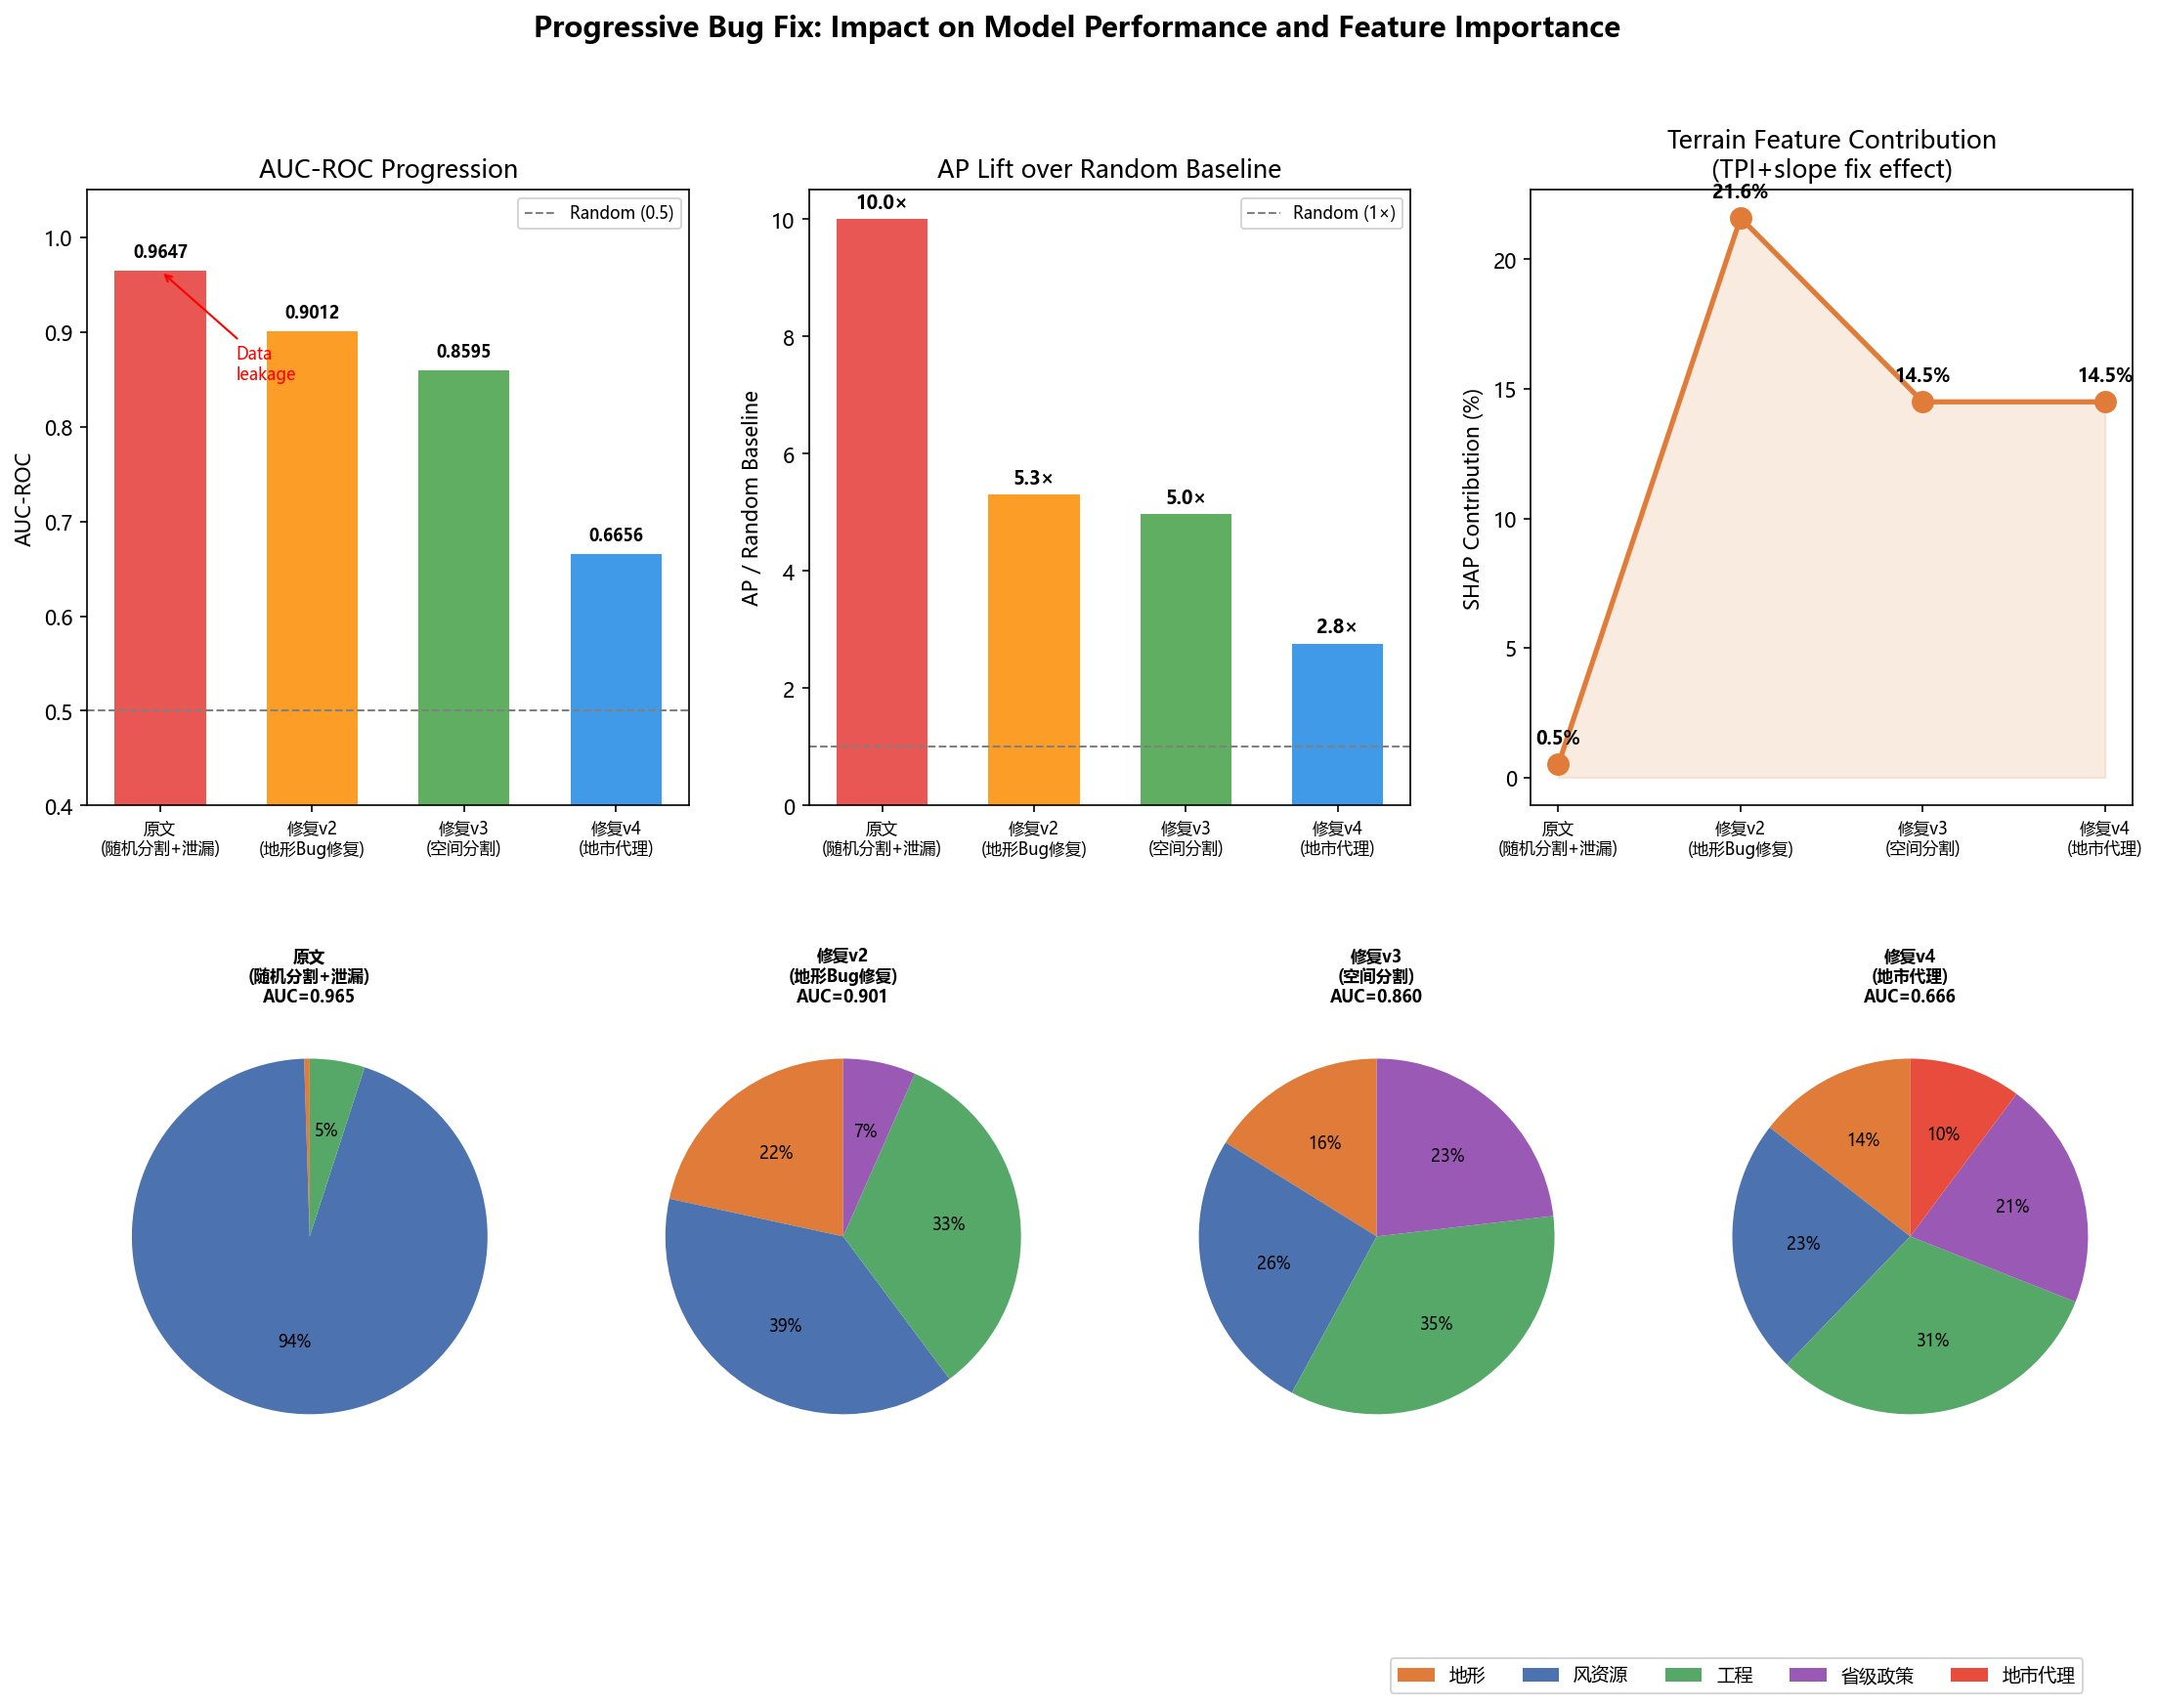
\includegraphics[width=0.95\textwidth]{progressive_fix_summary.png}
\caption{渐进式方案优化对模型性能与特征重要性的影响}
\label{fig:bugfix}
\end{figure}

% ── 参考文献 ─────────────────────────────────────────────
\begin{thebibliography}{99}

\bibitem{bilgili2024}
Bilgili M, et al.
Wind farm site selection using XGBoost with SHAP explainability.
\textit{Energy Conversion and Management}.
2024;309:118441.

\bibitem{chen2026}
Chen X, et al.
Spatially explicit wind farm siting probability across China at 1\,km.
\textit{Renewable Energy}.
2026;218:115406.

\bibitem{buster2024}
Buster G, et al.
Extraction of wind turbine setback ordinances using LLMs.
\textit{Nature Energy}.
2024;9(3):312--321.

\bibitem{li2023}
Li Y, et al.
BERT-based classification of Chinese energy policy texts.
\textit{Energy Policy}.
2023;181:113712.

\bibitem{xu2020}
Xu Z, et al.
GIS-based MCDM wind farm site selection in China.
\textit{Renewable Energy}.
2020;165:987--1001.

\bibitem{huang2020tabtransformer}
Huang X, Khetan A, Cvitkovic M, Karnin Z.
TabTransformer: tabular data modeling using contextual embeddings.
\textit{arXiv preprint arXiv:2012.06678}.
2020.

\bibitem{chen2018gradnorm}
Chen Z, Badrinarayanan V, Lee C-Y, Rabinovich A.
GradNorm: gradient normalization for adaptive loss balancing
in deep multitask networks.
In: \textit{Proceedings of the 35th International Conference on
Machine Learning (ICML)}.
2018:794--803.

\bibitem{ndrc2022}
国家发展改革委, 国家能源局.
《"十四五"可再生能源发展规划》（发改能源〔2021〕1445号）.
北京: 国家发展改革委; 2022.

\bibitem{ndrc2026}
国家发展改革委.
《中华人民共和国国民经济和社会发展第十五个五年规划纲要》.
北京: 国家发展改革委; 2026年3月.
\url{https://www.ndrc.gov.cn/fggz/fzzlgh/gjfzgh/202603/U020260317369114704096.pdf}

\bibitem{hersbach2020}
Hersbach H, Bell B, Berrisford P, et al.
The ERA5 global reanalysis.
\textit{Quarterly Journal of the Royal Meteorological Society}.
2020;146(730):1999--2049.

\bibitem{osm2023}
OpenStreetMap contributors.
Planet dump [Internet].
2023 [cited 2023 Dec].
Available from: \url{https://planet.openstreetmap.org}

\bibitem{devlin2019}
Devlin J, Chang M-W, Lee K, Toutanova K.
BERT: pre-training of deep bidirectional transformers for
language understanding.
In: \textit{Proceedings of NAACL-HLT}.
Minneapolis, MN: Association for Computational Linguistics;
2019:4171--4186.

\bibitem{hu2022}
Hu EJ, Shen Y, Wallis P, Allen-Zhu Z, Li Y,
Wang S, Wang L, Chen W.
LoRA: low-rank adaptation of large language models.
In: \textit{International Conference on Learning Representations
(ICLR)}.
2022. arXiv:2106.09685.

\bibitem{vaswani2017}
Vaswani A, Shazeer N, Parmar N, Uszkoreit J, Jones L,
Gomez AN, Kaiser {\L}, Polosukhin I.
Attention is all you need.
In: \textit{Advances in Neural Information Processing Systems
(NeurIPS)}.
2017;30:5998--6008.

\bibitem{lundberg2017}
Lundberg SM, Lee S-I.
A unified approach to interpreting model predictions.
In: \textit{Advances in Neural Information Processing Systems
(NeurIPS)}.
2017;30:4765--4774.

\bibitem{ester1996}
Ester M, Kriegel H-P, Sander J, Xu X.
A density-based algorithm for discovering clusters in large
spatial databases with noise.
In: \textit{Proceedings of the 2nd International Conference on
Knowledge Discovery and Data Mining (KDD)}.
Portland, OR: AAAI Press;
1996:226--231.

\bibitem{loshchilov2019}
Loshchilov I, Hutter F.
Decoupled weight decay regularization.
In: \textit{7th International Conference on Learning Representations
(ICLR)}.
New Orleans, LA, 2019.

\bibitem{jung2021}
Jung C, Schindler D.
Wind speed distributions used in wind energy assessment: a review.
\textit{Frontiers in Energy Research}.
2021;9:769920.

\bibitem{he2023}
He G, Lin J, Sifuentes F, Liu X, Abhyankar N, Phadke A.
Accelerating the energy transition towards photovoltaic
and wind in China.
\textit{Nature}.
2023;619:885--892.

\bibitem{zhong2022}
Zhong W, Qu X, Lv Q.
Toward carbon neutrality and China's 14th Five-Year Plan:
clean energy transition, sustainable urban development,
and investment priorities.
\textit{Sustainable Cities and Society}.
2022;87:104231.

\bibitem{wu2022}
Wu B, Yao S, Shen Y.
A review of GIS-based multi-criteria wind farm site selection methods.
\textit{Renewable and Sustainable Energy Reviews}.
2022;168:112753.

\bibitem{qiu2025gated}
Qiu Z, Wang Z, Zheng B, et al.
Gated attention for large language models: Non-linearity, sparsity,
and attention-sink-free.
\textit{arXiv preprint arXiv:2505.06708}. 2025.

\bibitem{chen2022scada}
Chen Y, Xu J.
Solar and wind power data from the Chinese State Grid
Renewable Energy Generation Forecasting Competition.
\textit{Scientific Data}.
2022;9:577.

\bibitem{jurasz2025}
Amsharuk A, \L aska G, Y\"{u}ksel K, Madlener R.
Machine learning-driven site selection for wind farms in Poland.
\textit{Energies}.
2025;18(22):6038.

\bibitem{ruan2025}
Ruan Z, Wang Y, Lu X, et al.
A systems-oriented review of China's wind and solar power
development toward carbon neutrality.
\textit{Technology Review for Carbon Neutrality}.
2025;1:9550010.

\bibitem{nepa2025}
Meyur R, Phan HD, Hayashi KB, et al.
Benchmarking LLMs for environmental review and permitting.
In: \textit{KDD 2025 Workshop SciSocLLM}; 2025.
arXiv:2407.07321.

\bibitem{bilgili2024xai}
Bilgili A, Arda T, Kilic B.
Explainability in wind farm planning: a machine learning
framework for automatic site selection of wind farms.
\textit{Energy Conversion and Management}.
2024;309:118441.

\bibitem{superres2025}
Ding JW, Hsieh IYL.
Super-resolution wind mapping with deep learning for scalable
renewable energy planning.
\textit{Communications Earth \& Environment}.
2026;7:51.


\bibitem{chen2016huline}
Chen M, Gong Y, Li Y, Lu D, Zhang H.
Population distribution and urbanization on both sides of the
Hu Huanyong Line: answers to the Premier's questions.
\textit{Journal of Geographical Sciences}.
2016;26(11):1593--1610.

\bibitem{zhao2023windchina}
Zhao M, Shi H, Chen X, et al.
Surface wind speed changes and their potential impact on wind
energy resources across China during 1961--2021.
\textit{GeoHealth}.
2023;7(9):e2023GH000861.

\bibitem{peft2025lora}
Hadji-Kyriacou A, Arandjelovic O.
Parameter-efficient fine-tuning for low-resource text
classification: a comparative study of LoRA, IA3, and ReFT.
\textit{Frontiers in Big Data}.
2025;8:1677331.
\bibitem{gbt19963}
National Energy Administration of China.
Technical rule for connecting wind farm to power system.
Part 1: onshore wind power.
\textit{GB/T 19963.1--2021}.
Beijing: Standardization Administration of China; 2021.

\bibitem{bonnier2024tabtext}
Bonnier T.
Revisiting multimodal transformers for tabular data with
text fields.
In: \textit{Findings of the Association for Computational
Linguistics: ACL 2024}.
Bangkok; August 2024.

\end{thebibliography}

\end{CJK}
\end{document}